\documentclass[twoside]{book}

% Packages required by doxygen
\usepackage{fixltx2e}
\usepackage{calc}
\usepackage{doxygen}
\usepackage[export]{adjustbox} % also loads graphicx
\usepackage{graphicx}
\usepackage[utf8]{inputenc}
\usepackage{makeidx}
\usepackage{multicol}
\usepackage{multirow}
\PassOptionsToPackage{warn}{textcomp}
\usepackage{textcomp}
\usepackage[nointegrals]{wasysym}
\usepackage[table]{xcolor}

% Font selection
\usepackage[T1]{fontenc}
\usepackage[scaled=.90]{helvet}
\usepackage{courier}
\usepackage{amssymb}
\usepackage{sectsty}
\renewcommand{\familydefault}{\sfdefault}
\allsectionsfont{%
  \fontseries{bc}\selectfont%
  \color{darkgray}%
}
\renewcommand{\DoxyLabelFont}{%
  \fontseries{bc}\selectfont%
  \color{darkgray}%
}
\newcommand{\+}{\discretionary{\mbox{\scriptsize$\hookleftarrow$}}{}{}}

% Page & text layout
\usepackage{geometry}
\geometry{%
  a4paper,%
  top=2.5cm,%
  bottom=2.5cm,%
  left=2.5cm,%
  right=2.5cm%
}
\tolerance=750
\hfuzz=15pt
\hbadness=750
\setlength{\emergencystretch}{15pt}
\setlength{\parindent}{0cm}
\setlength{\parskip}{3ex plus 2ex minus 2ex}
\makeatletter
\renewcommand{\paragraph}{%
  \@startsection{paragraph}{4}{0ex}{-1.0ex}{1.0ex}{%
    \normalfont\normalsize\bfseries\SS@parafont%
  }%
}
\renewcommand{\subparagraph}{%
  \@startsection{subparagraph}{5}{0ex}{-1.0ex}{1.0ex}{%
    \normalfont\normalsize\bfseries\SS@subparafont%
  }%
}
\makeatother

% Headers & footers
\usepackage{fancyhdr}
\pagestyle{fancyplain}
\fancyhead[LE]{\fancyplain{}{\bfseries\thepage}}
\fancyhead[CE]{\fancyplain{}{}}
\fancyhead[RE]{\fancyplain{}{\bfseries\leftmark}}
\fancyhead[LO]{\fancyplain{}{\bfseries\rightmark}}
\fancyhead[CO]{\fancyplain{}{}}
\fancyhead[RO]{\fancyplain{}{\bfseries\thepage}}
\fancyfoot[LE]{\fancyplain{}{}}
\fancyfoot[CE]{\fancyplain{}{}}
\fancyfoot[RE]{\fancyplain{}{\bfseries\scriptsize Generated by Doxygen }}
\fancyfoot[LO]{\fancyplain{}{\bfseries\scriptsize Generated by Doxygen }}
\fancyfoot[CO]{\fancyplain{}{}}
\fancyfoot[RO]{\fancyplain{}{}}
\renewcommand{\footrulewidth}{0.4pt}
\renewcommand{\chaptermark}[1]{%
  \markboth{#1}{}%
}
\renewcommand{\sectionmark}[1]{%
  \markright{\thesection\ #1}%
}

% Indices & bibliography
\usepackage{natbib}
\usepackage[titles]{tocloft}
\setcounter{tocdepth}{3}
\setcounter{secnumdepth}{5}
\makeindex

% Hyperlinks (required, but should be loaded last)
\usepackage{ifpdf}
\ifpdf
  \usepackage[pdftex,pagebackref=true]{hyperref}
\else
  \usepackage[ps2pdf,pagebackref=true]{hyperref}
\fi
\hypersetup{%
  colorlinks=true,%
  linkcolor=blue,%
  citecolor=blue,%
  unicode%
}

% Custom commands
\newcommand{\clearemptydoublepage}{%
  \newpage{\pagestyle{empty}\cleardoublepage}%
}

\usepackage{caption}
\captionsetup{labelsep=space,justification=centering,font={bf},singlelinecheck=off,skip=4pt,position=top}

%===== C O N T E N T S =====

\begin{document}

% Titlepage & ToC
\hypersetup{pageanchor=false,
             bookmarksnumbered=true,
             pdfencoding=unicode
            }
\pagenumbering{alph}
\begin{titlepage}
\vspace*{7cm}
\begin{center}%
{\Large Spider-\/\+Client }\\
\vspace*{1cm}
{\large Generated by Doxygen 1.8.13}\\
\end{center}
\end{titlepage}
\clearemptydoublepage
\pagenumbering{roman}
\tableofcontents
\clearemptydoublepage
\pagenumbering{arabic}
\hypersetup{pageanchor=true}

%--- Begin generated contents ---
\chapter{Namespace Index}
\section{Namespace List}
Here is a list of all documented namespaces with brief descriptions\+:\begin{DoxyCompactList}
\item\contentsline{section}{\hyperlink{namespace_spider}{Spider} }{\pageref{namespace_spider}}{}
\item\contentsline{section}{\hyperlink{namespace_spider_1_1_event}{Spider\+::\+Event} }{\pageref{namespace_spider_1_1_event}}{}
\end{DoxyCompactList}

\chapter{Hierarchical Index}
\section{Class Hierarchy}
This inheritance list is sorted roughly, but not completely, alphabetically\+:\begin{DoxyCompactList}
\item \contentsline{section}{ts\+:\+:Client\+Manager}{\pageref{classts_1_1_client_manager}}{}
\item \contentsline{section}{ts\+:\+:common\+:\+:tcp\+:\+:Client\+Socket}{\pageref{classts_1_1common_1_1tcp_1_1_client_socket}}{}
\item \contentsline{section}{ts\+:\+:common\+:\+:udp\+:\+:Client\+Socket}{\pageref{classts_1_1common_1_1udp_1_1_client_socket}}{}
\begin{DoxyCompactList}
\item \contentsline{section}{ts\+:\+:common\+:\+:udp\+:\+:Server\+Socket}{\pageref{classts_1_1common_1_1udp_1_1_server_socket}}{}
\end{DoxyCompactList}
\item enable\+\_\+shared\+\_\+from\+\_\+this\begin{DoxyCompactList}
\item \contentsline{section}{ts\+:\+:Client}{\pageref{classts_1_1_client}}{}
\end{DoxyCompactList}
\item exception\begin{DoxyCompactList}
\item \contentsline{section}{ts\+:\+:Program\+Option\+Exception}{\pageref{classts_1_1_program_option_exception}}{}
\end{DoxyCompactList}
\item \contentsline{section}{ts\+:\+:I\+Data\+Recorder}{\pageref{classts_1_1_i_data_recorder}}{}
\begin{DoxyCompactList}
\item \contentsline{section}{ts\+:\+:Sqlite\+Data\+Recorder}{\pageref{classts_1_1_sqlite_data_recorder}}{}
\end{DoxyCompactList}
\item \contentsline{section}{ts\+:\+:common\+:\+:Json\+Parser}{\pageref{classts_1_1common_1_1_json_parser}}{}
\item noncopyable\begin{DoxyCompactList}
\item \contentsline{section}{ts\+:\+:Client}{\pageref{classts_1_1_client}}{}
\end{DoxyCompactList}
\item \contentsline{section}{ts\+:\+:Option}{\pageref{structts_1_1_option}}{}
\item \contentsline{section}{ts\+:\+:common\+:\+:Packet}{\pageref{structts_1_1common_1_1_packet}}{}
\item \contentsline{section}{ts\+:\+:common\+:\+:Packet\+Body}{\pageref{structts_1_1common_1_1_packet_body}}{}
\item \contentsline{section}{ts\+:\+:common\+:\+:Packet\+Header}{\pageref{structts_1_1common_1_1_packet_header}}{}
\item \contentsline{section}{ts\+:\+:common\+:\+:Packet\+Manager}{\pageref{classts_1_1common_1_1_packet_manager}}{}
\item \contentsline{section}{ts\+:\+:Program\+Option}{\pageref{classts_1_1_program_option}}{}
\item \contentsline{section}{ts\+:\+:common\+:\+:Request}{\pageref{structts_1_1common_1_1_request}}{}
\begin{DoxyCompactList}
\item \contentsline{section}{ts\+:\+:common\+:\+:Auth\+Req}{\pageref{structts_1_1common_1_1_auth_req}}{}
\item \contentsline{section}{ts\+:\+:common\+:\+:Auth\+Resp}{\pageref{structts_1_1common_1_1_auth_resp}}{}
\item \contentsline{section}{ts\+:\+:common\+:\+:Click\+Activity\+Req}{\pageref{structts_1_1common_1_1_click_activity_req}}{}
\item \contentsline{section}{ts\+:\+:common\+:\+:Command\+Req}{\pageref{structts_1_1common_1_1_command_req}}{}
\item \contentsline{section}{ts\+:\+:common\+:\+:Disconnect\+Req}{\pageref{structts_1_1common_1_1_disconnect_req}}{}
\item \contentsline{section}{ts\+:\+:common\+:\+:Error\+Req}{\pageref{structts_1_1common_1_1_error_req}}{}
\item \contentsline{section}{ts\+:\+:common\+:\+:Key\+Info\+Req}{\pageref{structts_1_1common_1_1_key_info_req}}{}
\item \contentsline{section}{ts\+:\+:common\+:\+:Notice\+Receipt\+Req}{\pageref{structts_1_1common_1_1_notice_receipt_req}}{}
\item \contentsline{section}{ts\+:\+:common\+:\+:Ping\+Req}{\pageref{structts_1_1common_1_1_ping_req}}{}
\item \contentsline{section}{ts\+:\+:common\+:\+:Ping\+Resp}{\pageref{structts_1_1common_1_1_ping_resp}}{}
\end{DoxyCompactList}
\item \contentsline{section}{ts\+:\+:Request\+Handler}{\pageref{classts_1_1_request_handler}}{}
\item \contentsline{section}{ts\+:\+:common\+:\+:Request\+Manager}{\pageref{classts_1_1common_1_1_request_manager}}{}
\item \contentsline{section}{ts\+:\+:Server\+Network}{\pageref{classts_1_1_server_network}}{}
\item \contentsline{section}{ts\+:\+:common\+:\+:tcp\+:\+:Server\+Socket}{\pageref{classts_1_1common_1_1tcp_1_1_server_socket}}{}
\item \contentsline{section}{ts\+:\+:common\+:\+:Singleton$<$ T\+Singleton $>$}{\pageref{classts_1_1common_1_1_singleton}}{}
\item \contentsline{section}{ts\+:\+:common\+:\+:Singleton$<$ Debug $>$}{\pageref{classts_1_1common_1_1_singleton}}{}
\begin{DoxyCompactList}
\item \contentsline{section}{ts\+:\+:common\+:\+:Debug}{\pageref{classts_1_1common_1_1_debug}}{}
\end{DoxyCompactList}
\item \contentsline{section}{ts\+:\+:common\+:\+:Singleton$<$ Spider\+Server $>$}{\pageref{classts_1_1common_1_1_singleton}}{}
\begin{DoxyCompactList}
\item \contentsline{section}{ts\+:\+:Spider\+Server}{\pageref{classts_1_1_spider_server}}{}
\end{DoxyCompactList}
\end{DoxyCompactList}

\chapter{Class Index}
\section{Class List}
Here are the classes, structs, unions and interfaces with brief descriptions\+:\begin{DoxyCompactList}
\item\contentsline{section}{\hyperlink{class_spider_1_1ssl_1_1_a_e_s}{Spider\+::ssl\+::\+A\+ES} \\*Encapsulation of the open\+S\+SL \hyperlink{class_spider_1_1ssl_1_1_a_e_s}{A\+ES} system }{\pageref{class_spider_1_1ssl_1_1_a_e_s}}{}
\item\contentsline{section}{\hyperlink{class_spider_1_1_event_1_1_click}{Spider\+::\+Event\+::\+Click} }{\pageref{class_spider_1_1_event_1_1_click}}{}
\item\contentsline{section}{\hyperlink{class_c_lick}{C\+Lick} \\*Handle click events }{\pageref{class_c_lick}}{}
\item\contentsline{section}{\hyperlink{struct_spider_1_1_event_1_1_click_coord}{Spider\+::\+Event\+::\+Click\+Coord} \\*Define the click coordonate }{\pageref{struct_spider_1_1_event_1_1_click_coord}}{}
\item\contentsline{section}{\hyperlink{classts_1_1common_1_1tcp_1_1_client_socket}{ts\+::common\+::tcp\+::\+Client\+Socket} }{\pageref{classts_1_1common_1_1tcp_1_1_client_socket}}{}
\item\contentsline{section}{\hyperlink{class_spider_1_1_core_exception}{Spider\+::\+Core\+Exception} \\*Core exception class }{\pageref{class_spider_1_1_core_exception}}{}
\item\contentsline{section}{\hyperlink{class_spider_1_1_d_b_exception}{Spider\+::\+D\+B\+Exception} }{\pageref{class_spider_1_1_d_b_exception}}{}
\item\contentsline{section}{\hyperlink{class_spider_1_1_d_b_1_1_d_b_handler}{Spider\+::\+D\+B\+::\+D\+B\+Handler} }{\pageref{class_spider_1_1_d_b_1_1_d_b_handler}}{}
\item\contentsline{section}{\hyperlink{class_spider_1_1_event_1_1_event_handler}{Spider\+::\+Event\+::\+Event\+Handler} \\*Handle events }{\pageref{class_spider_1_1_event_1_1_event_handler}}{}
\item\contentsline{section}{\hyperlink{class_spider_1_1_event_1_1_event_queue}{Spider\+::\+Event\+::\+Event\+Queue} \\*Queue system for \hyperlink{namespace_spider}{Spider} events }{\pageref{class_spider_1_1_event_1_1_event_queue}}{}
\item\contentsline{section}{\hyperlink{class_spider_1_1_event_1_1_i_event}{Spider\+::\+Event\+::\+I\+Event} \\*\hyperlink{namespace_spider_1_1_event}{Event} interface }{\pageref{class_spider_1_1_event_1_1_i_event}}{}
\item\contentsline{section}{\hyperlink{class_spider_1_1_event_1_1_keyboard}{Spider\+::\+Event\+::\+Keyboard} \\*\hyperlink{class_spider_1_1_event_1_1_keyboard}{Keyboard} Handler }{\pageref{class_spider_1_1_event_1_1_keyboard}}{}
\item\contentsline{section}{\hyperlink{class_spider_1_1_core_1_1_key_reader}{Spider\+::\+Core\+::\+Key\+Reader} \\*Read event }{\pageref{class_spider_1_1_core_1_1_key_reader}}{}
\item\contentsline{section}{\hyperlink{structts_1_1common_1_1_packet}{ts\+::common\+::\+Packet} }{\pageref{structts_1_1common_1_1_packet}}{}
\item\contentsline{section}{\hyperlink{structts_1_1common_1_1_packet_body}{ts\+::common\+::\+Packet\+Body} }{\pageref{structts_1_1common_1_1_packet_body}}{}
\item\contentsline{section}{\hyperlink{structts_1_1common_1_1_packet_header}{ts\+::common\+::\+Packet\+Header} }{\pageref{structts_1_1common_1_1_packet_header}}{}
\item\contentsline{section}{\hyperlink{classts_1_1common_1_1_packet_manager}{ts\+::common\+::\+Packet\+Manager} }{\pageref{classts_1_1common_1_1_packet_manager}}{}
\item\contentsline{section}{\hyperlink{class_spider_1_1_event_1_1_request}{Spider\+::\+Event\+::\+Request} \\*\hyperlink{class_spider_1_1_event_1_1_request}{Request} informations container }{\pageref{class_spider_1_1_event_1_1_request}}{}
\item\contentsline{section}{\hyperlink{class_spider_1_1ssl_1_1_r_s_a_keys}{Spider\+::ssl\+::\+R\+S\+A\+Keys} \\*Encapsulation of the open\+S\+SL one-\/way encryption system }{\pageref{class_spider_1_1ssl_1_1_r_s_a_keys}}{}
\item\contentsline{section}{\hyperlink{class_spider_1_1ssl_1_1_sha}{Spider\+::ssl\+::\+Sha} \\*Encapsulation of the open\+S\+SL one-\/way encryption system }{\pageref{class_spider_1_1ssl_1_1_sha}}{}
\item\contentsline{section}{\hyperlink{class_spider_1_1_core_1_1_spider}{Spider\+::\+Core\+::\+Spider} \\*Project main class }{\pageref{class_spider_1_1_core_1_1_spider}}{}
\item\contentsline{section}{\hyperlink{class_spider_1_1_spider_exception}{Spider\+::\+Spider\+Exception} \\*Exception interface }{\pageref{class_spider_1_1_spider_exception}}{}
\item\contentsline{section}{\hyperlink{class_spider_1_1_event_1_1_user_activity}{Spider\+::\+Event\+::\+User\+Activity} \\*\hyperlink{class_spider_1_1_event_1_1_user_activity}{User\+Activity} Handler }{\pageref{class_spider_1_1_event_1_1_user_activity}}{}
\end{DoxyCompactList}

\chapter{File Index}
\section{File List}
Here is a list of all documented files with brief descriptions\+:\begin{DoxyCompactList}
\item\contentsline{section}{Core/\hyperlink{_key_reader_8hpp}{Key\+Reader.\+hpp} }{\pageref{_key_reader_8hpp}}{}
\item\contentsline{section}{Core/\hyperlink{_spider_8hpp}{Spider.\+hpp} }{\pageref{_spider_8hpp}}{}
\item\contentsline{section}{D\+B/\hyperlink{_d_b_handler_8hpp}{D\+B\+Handler.\+hpp} }{\pageref{_d_b_handler_8hpp}}{}
\item\contentsline{section}{Event/{\bfseries Click.\+hpp} }{\pageref{_click_8hpp}}{}
\item\contentsline{section}{Event/\hyperlink{_click_association_8hpp}{Click\+Association.\+hpp} }{\pageref{_click_association_8hpp}}{}
\item\contentsline{section}{Event/\hyperlink{_event_8hpp}{Event.\+hpp} }{\pageref{_event_8hpp}}{}
\item\contentsline{section}{Event/\hyperlink{_event_handler_8hpp}{Event\+Handler.\+hpp} }{\pageref{_event_handler_8hpp}}{}
\item\contentsline{section}{Event/\hyperlink{_event_queue_8hpp}{Event\+Queue.\+hpp} }{\pageref{_event_queue_8hpp}}{}
\item\contentsline{section}{Event/\hyperlink{_i_event_8hpp}{I\+Event.\+hpp} }{\pageref{_i_event_8hpp}}{}
\item\contentsline{section}{Event/{\bfseries Keyboard.\+hpp} }{\pageref{_keyboard_8hpp}}{}
\item\contentsline{section}{Event/{\bfseries Request.\+hpp} }{\pageref{_request_8hpp}}{}
\item\contentsline{section}{Event/\hyperlink{_user_activity_8hpp}{User\+Activity.\+hpp} }{\pageref{_user_activity_8hpp}}{}
\item\contentsline{section}{Exception/\hyperlink{_core_exception_8hpp}{Core\+Exception.\+hpp} }{\pageref{_core_exception_8hpp}}{}
\item\contentsline{section}{Exception/\hyperlink{_d_b_exception_8hpp}{D\+B\+Exception.\+hpp} }{\pageref{_d_b_exception_8hpp}}{}
\item\contentsline{section}{Exception/\hyperlink{_spider_exception_8hpp}{Spider\+Exception.\+hpp} }{\pageref{_spider_exception_8hpp}}{}
\item\contentsline{section}{Socket/{\bfseries Packet.\+hpp} }{\pageref{_packet_8hpp}}{}
\item\contentsline{section}{Socket/{\bfseries Packet\+Manager.\+hpp} }{\pageref{_packet_manager_8hpp}}{}
\item\contentsline{section}{Socket/{\bfseries Tcp\+Client\+Socket.\+hpp} }{\pageref{_tcp_client_socket_8hpp}}{}
\item\contentsline{section}{ssl/\hyperlink{_a_e_s_8hpp}{A\+E\+S.\+hpp} }{\pageref{_a_e_s_8hpp}}{}
\item\contentsline{section}{ssl/\hyperlink{_r_s_a_keys_8hpp}{R\+S\+A\+Keys.\+hpp} }{\pageref{_r_s_a_keys_8hpp}}{}
\item\contentsline{section}{ssl/\hyperlink{_sha_8hpp}{Sha.\+hpp} }{\pageref{_sha_8hpp}}{}
\item\contentsline{section}{ssl/\hyperlink{ssl_8hpp}{ssl.\+hpp} }{\pageref{ssl_8hpp}}{}
\end{DoxyCompactList}

\chapter{Namespace Documentation}
\hypertarget{namespace_spider}{}\section{Spider Namespace Reference}
\label{namespace_spider}\index{Spider@{Spider}}
\subsection*{Namespaces}
\begin{DoxyCompactItemize}
\item 
 \hyperlink{namespace_spider_1_1_event}{Event}
\end{DoxyCompactItemize}
\subsection*{Classes}
\begin{DoxyCompactItemize}
\item 
class \hyperlink{class_spider_1_1_core_exception}{Core\+Exception}
\begin{DoxyCompactList}\small\item\em Core exception class. \end{DoxyCompactList}\item 
class \hyperlink{class_spider_1_1_d_b_exception}{D\+B\+Exception}
\item 
class \hyperlink{class_spider_1_1_spider_exception}{Spider\+Exception}
\begin{DoxyCompactList}\small\item\em Exception interface. \end{DoxyCompactList}\end{DoxyCompactItemize}


\subsection{Detailed Description}
\hyperlink{namespace_spider}{Spider} 
\hypertarget{namespace_spider_1_1_event}{}\section{Spider\+:\+:Event Namespace Reference}
\label{namespace_spider_1_1_event}\index{Spider\+::\+Event@{Spider\+::\+Event}}
\subsection*{Classes}
\begin{DoxyCompactItemize}
\item 
class \hyperlink{class_spider_1_1_event_1_1_click}{Click}
\item 
struct \hyperlink{struct_spider_1_1_event_1_1_click_coord}{Click\+Coord}
\begin{DoxyCompactList}\small\item\em Define the click coordonate. \end{DoxyCompactList}\item 
class \hyperlink{class_spider_1_1_event_1_1_event_handler}{Event\+Handler}
\begin{DoxyCompactList}\small\item\em Handle events. \end{DoxyCompactList}\item 
class \hyperlink{class_spider_1_1_event_1_1_event_queue}{Event\+Queue}
\begin{DoxyCompactList}\small\item\em Queue system for \hyperlink{namespace_spider}{Spider} events. \end{DoxyCompactList}\item 
class \hyperlink{class_spider_1_1_event_1_1_i_event}{I\+Event}
\begin{DoxyCompactList}\small\item\em \hyperlink{namespace_spider_1_1_event}{Event} interface. \end{DoxyCompactList}\item 
class \hyperlink{class_spider_1_1_event_1_1_keyboard}{Keyboard}
\begin{DoxyCompactList}\small\item\em \hyperlink{class_spider_1_1_event_1_1_keyboard}{Keyboard} Handler. \end{DoxyCompactList}\item 
class \hyperlink{class_spider_1_1_event_1_1_request}{Request}
\begin{DoxyCompactList}\small\item\em \hyperlink{class_spider_1_1_event_1_1_request}{Request} informations container. \end{DoxyCompactList}\item 
class \hyperlink{class_spider_1_1_event_1_1_user_activity}{User\+Activity}
\begin{DoxyCompactList}\small\item\em \hyperlink{class_spider_1_1_event_1_1_user_activity}{User\+Activity} Handler. \end{DoxyCompactList}\end{DoxyCompactItemize}
\subsection*{Enumerations}
\begin{DoxyCompactItemize}
\item 
\mbox{\Hypertarget{namespace_spider_1_1_event_ae178d39ebb8937d04ffe6ead8f306fd0}\label{namespace_spider_1_1_event_ae178d39ebb8937d04ffe6ead8f306fd0}} 
enum \hyperlink{namespace_spider_1_1_event_ae178d39ebb8937d04ffe6ead8f306fd0}{Click\+Type} \{ {\bfseries L\+E\+F\+T\+\_\+\+C\+L\+I\+CK}, 
{\bfseries M\+I\+D\+D\+L\+E\+\_\+\+C\+L\+I\+CK}, 
{\bfseries R\+I\+G\+H\+T\+\_\+\+C\+L\+I\+CK}, 
{\bfseries N\+O\+NE}
 \}\begin{DoxyCompactList}\small\item\em Define the type of the click from the user. \end{DoxyCompactList}
\end{DoxyCompactItemize}
\subsection*{Variables}
\begin{DoxyCompactItemize}
\item 
std\+::unordered\+\_\+map$<$ int, \hyperlink{namespace_spider_1_1_event_ae178d39ebb8937d04ffe6ead8f306fd0}{Event\+::\+Click\+Type} $>$ {\bfseries associative\+Click}
\end{DoxyCompactItemize}


\subsection{Detailed Description}
\hyperlink{namespace_spider_1_1_event}{Event} 

\subsection{Variable Documentation}
\mbox{\Hypertarget{namespace_spider_1_1_event_a18a7153c12e999d71c1490dbc9c464d8}\label{namespace_spider_1_1_event_a18a7153c12e999d71c1490dbc9c464d8}} 
\index{Spider\+::\+Event@{Spider\+::\+Event}!associative\+Click@{associative\+Click}}
\index{associative\+Click@{associative\+Click}!Spider\+::\+Event@{Spider\+::\+Event}}
\subsubsection{\texorpdfstring{associative\+Click}{associativeClick}}
{\footnotesize\ttfamily std\+::unordered\+\_\+map$<$int, \hyperlink{namespace_spider_1_1_event_ae178d39ebb8937d04ffe6ead8f306fd0}{Event\+::\+Click\+Type}$>$ Spider\+::\+Event\+::associative\+Click}

{\bfseries Initial value\+:}
\begin{DoxyCode}
\{
        \{ VK\_LBUTTON, Event::LEFT\_CLICK \},
        \{ VK\_MBUTTON, Event::MIDDLE\_CLICK \},
        \{ VK\_RBUTTON, Event::RIGHT\_CLICK \}
    \}
\end{DoxyCode}

\chapter{Class Documentation}
\hypertarget{class_spider_1_1ssl_1_1_a_e_s}{}\section{Spider\+:\+:ssl\+:\+:A\+ES Class Reference}
\label{class_spider_1_1ssl_1_1_a_e_s}\index{Spider\+::ssl\+::\+A\+ES@{Spider\+::ssl\+::\+A\+ES}}


Encapsulation of the open\+S\+SL \hyperlink{class_spider_1_1ssl_1_1_a_e_s}{A\+ES} system.  




{\ttfamily \#include $<$A\+E\+S.\+hpp$>$}

\subsection*{Public Member Functions}
\begin{DoxyCompactItemize}
\item 
\mbox{\Hypertarget{class_spider_1_1ssl_1_1_a_e_s_a8eaa642dde56e252f2a88428fc3964af}\label{class_spider_1_1ssl_1_1_a_e_s_a8eaa642dde56e252f2a88428fc3964af}} 
\hyperlink{class_spider_1_1ssl_1_1_a_e_s_a8eaa642dde56e252f2a88428fc3964af}{A\+ES} ()
\begin{DoxyCompactList}\small\item\em Default \hyperlink{class_spider_1_1ssl_1_1_a_e_s}{A\+ES} Class Constructor. \end{DoxyCompactList}\item 
\hyperlink{class_spider_1_1ssl_1_1_a_e_s_a9da7fa808bebcdb3042322a371473069}{A\+ES} (const \hyperlink{class_spider_1_1ssl_1_1_a_e_s}{A\+ES} \&key)
\begin{DoxyCompactList}\small\item\em \hyperlink{class_spider_1_1ssl_1_1_a_e_s}{A\+ES} class copy constructor. \end{DoxyCompactList}\item 
\hyperlink{class_spider_1_1ssl_1_1_a_e_s_ae588c5d1794e8cbe1cc74cf4ffc8b276}{A\+ES} (const unsigned char $\ast$key)
\begin{DoxyCompactList}\small\item\em Constructor that automatically loads a key from its path and is type. \end{DoxyCompactList}\item 
\hyperlink{class_spider_1_1ssl_1_1_a_e_s}{A\+ES} \& \hyperlink{class_spider_1_1ssl_1_1_a_e_s_a46a15236249277adc1b4b1961985d2bf}{operator=} (const \hyperlink{class_spider_1_1ssl_1_1_a_e_s}{A\+ES} \&key)
\begin{DoxyCompactList}\small\item\em Copy Operator, copy a key. \end{DoxyCompactList}\item 
bool \hyperlink{class_spider_1_1ssl_1_1_a_e_s_ad9014e425e6149e7006b8b309a933bc2}{operator==} (const \hyperlink{class_spider_1_1ssl_1_1_a_e_s}{A\+ES} \&key) const
\begin{DoxyCompactList}\small\item\em Equal operator, allows to know if two keys are equal. \end{DoxyCompactList}\item 
\mbox{\Hypertarget{class_spider_1_1ssl_1_1_a_e_s_aab6bae111d14ed5ec7fe0cefbb8ba3cc}\label{class_spider_1_1ssl_1_1_a_e_s_aab6bae111d14ed5ec7fe0cefbb8ba3cc}} 
\hyperlink{class_spider_1_1ssl_1_1_a_e_s_aab6bae111d14ed5ec7fe0cefbb8ba3cc}{$\sim$\+A\+ES} ()
\begin{DoxyCompactList}\small\item\em Default Destroyer. \end{DoxyCompactList}\item 
void \hyperlink{class_spider_1_1ssl_1_1_a_e_s_a3cba36653117622e01fedfafa9fb1c6a}{generate} ()
\begin{DoxyCompactList}\small\item\em Generates a new internal key of the class. \end{DoxyCompactList}\item 
void \hyperlink{class_spider_1_1ssl_1_1_a_e_s_a16b092b57a8906edc6845176eed10256}{affect} (const unsigned char $\ast$key)
\begin{DoxyCompactList}\small\item\em Assigns a key to the instance. \end{DoxyCompactList}\item 
\mbox{\Hypertarget{class_spider_1_1ssl_1_1_a_e_s_aa6c03237be40637cae04f0ec9161bc79}\label{class_spider_1_1ssl_1_1_a_e_s_aa6c03237be40637cae04f0ec9161bc79}} 
void \hyperlink{class_spider_1_1ssl_1_1_a_e_s_aa6c03237be40637cae04f0ec9161bc79}{clear} ()
\begin{DoxyCompactList}\small\item\em Removes the key without destroying the object. \end{DoxyCompactList}\item 
bool \hyperlink{class_spider_1_1ssl_1_1_a_e_s_a93e682bc36f5a52d75289fd43c2404f6}{is\+Initialize} () const
\begin{DoxyCompactList}\small\item\em Whether the key is initialized or not. \end{DoxyCompactList}\item 
unsigned char $\ast$ \hyperlink{class_spider_1_1ssl_1_1_a_e_s_af29f6f29119e34fcf27605ed85a3460d}{get} ()
\begin{DoxyCompactList}\small\item\em Extract the key from the class. \end{DoxyCompactList}\item 
bool \hyperlink{class_spider_1_1ssl_1_1_a_e_s_a9ed853ba70dba93ed28523a9dcd52d72}{read} (const std\+::string \&path)
\begin{DoxyCompactList}\small\item\em Read \hyperlink{class_spider_1_1ssl_1_1_a_e_s}{A\+ES} key in a file. \end{DoxyCompactList}\item 
void \hyperlink{class_spider_1_1ssl_1_1_a_e_s_ac4c9691e1fd1c250343ebe8206f26026}{write} (int fd)
\begin{DoxyCompactList}\small\item\em Write the key in a specific file director. \end{DoxyCompactList}\item 
std\+::string \hyperlink{class_spider_1_1ssl_1_1_a_e_s_a035de929280e43fed57eb5bbadab394f}{crypt} (const std\+::string \&data) const
\begin{DoxyCompactList}\small\item\em Encrypts data from a class key. \end{DoxyCompactList}\item 
std\+::string \hyperlink{class_spider_1_1ssl_1_1_a_e_s_a187c229df6c9e59b44c6148f5eac6177}{uncrypt} (const std\+::string \&data) const
\begin{DoxyCompactList}\small\item\em Decrypts data from class A\+E\+S\+Key. \end{DoxyCompactList}\end{DoxyCompactItemize}


\subsection{Detailed Description}
Encapsulation of the open\+S\+SL \hyperlink{class_spider_1_1ssl_1_1_a_e_s}{A\+ES} system. 

\begin{DoxyWarning}{Warning}
The \hyperlink{class_spider_1_1ssl_1_1_a_e_s}{A\+ES} key to a size defined by the open\+S\+Sl (A\+E\+S\+\_\+\+B\+L\+O\+C\+K\+\_\+\+S\+I\+ZE) 
\end{DoxyWarning}


\subsection{Constructor \& Destructor Documentation}
\mbox{\Hypertarget{class_spider_1_1ssl_1_1_a_e_s_a9da7fa808bebcdb3042322a371473069}\label{class_spider_1_1ssl_1_1_a_e_s_a9da7fa808bebcdb3042322a371473069}} 
\index{Spider\+::ssl\+::\+A\+ES@{Spider\+::ssl\+::\+A\+ES}!A\+ES@{A\+ES}}
\index{A\+ES@{A\+ES}!Spider\+::ssl\+::\+A\+ES@{Spider\+::ssl\+::\+A\+ES}}
\subsubsection{\texorpdfstring{A\+E\+S()}{AES()}\hspace{0.1cm}{\footnotesize\ttfamily [1/2]}}
{\footnotesize\ttfamily Spider\+::ssl\+::\+A\+E\+S\+::\+A\+ES (\begin{DoxyParamCaption}\item[{const \hyperlink{class_spider_1_1ssl_1_1_a_e_s}{A\+ES} \&}]{key }\end{DoxyParamCaption})}



\hyperlink{class_spider_1_1ssl_1_1_a_e_s}{A\+ES} class copy constructor. 


\begin{DoxyParams}{Parameters}
{\em key} & Key that will be copied \\
\hline
\end{DoxyParams}
\mbox{\Hypertarget{class_spider_1_1ssl_1_1_a_e_s_ae588c5d1794e8cbe1cc74cf4ffc8b276}\label{class_spider_1_1ssl_1_1_a_e_s_ae588c5d1794e8cbe1cc74cf4ffc8b276}} 
\index{Spider\+::ssl\+::\+A\+ES@{Spider\+::ssl\+::\+A\+ES}!A\+ES@{A\+ES}}
\index{A\+ES@{A\+ES}!Spider\+::ssl\+::\+A\+ES@{Spider\+::ssl\+::\+A\+ES}}
\subsubsection{\texorpdfstring{A\+E\+S()}{AES()}\hspace{0.1cm}{\footnotesize\ttfamily [2/2]}}
{\footnotesize\ttfamily Spider\+::ssl\+::\+A\+E\+S\+::\+A\+ES (\begin{DoxyParamCaption}\item[{const unsigned char $\ast$}]{key }\end{DoxyParamCaption})}



Constructor that automatically loads a key from its path and is type. 


\begin{DoxyParams}{Parameters}
{\em key} & Key in the form of a string \\
\hline
\end{DoxyParams}


\subsection{Member Function Documentation}
\mbox{\Hypertarget{class_spider_1_1ssl_1_1_a_e_s_a16b092b57a8906edc6845176eed10256}\label{class_spider_1_1ssl_1_1_a_e_s_a16b092b57a8906edc6845176eed10256}} 
\index{Spider\+::ssl\+::\+A\+ES@{Spider\+::ssl\+::\+A\+ES}!affect@{affect}}
\index{affect@{affect}!Spider\+::ssl\+::\+A\+ES@{Spider\+::ssl\+::\+A\+ES}}
\subsubsection{\texorpdfstring{affect()}{affect()}}
{\footnotesize\ttfamily void Spider\+::ssl\+::\+A\+E\+S\+::affect (\begin{DoxyParamCaption}\item[{const unsigned char $\ast$}]{key }\end{DoxyParamCaption})\hspace{0.3cm}{\ttfamily [inline]}}



Assigns a key to the instance. 


\begin{DoxyParams}{Parameters}
{\em key} & Reference key to be used \\
\hline
\end{DoxyParams}
\mbox{\Hypertarget{class_spider_1_1ssl_1_1_a_e_s_a035de929280e43fed57eb5bbadab394f}\label{class_spider_1_1ssl_1_1_a_e_s_a035de929280e43fed57eb5bbadab394f}} 
\index{Spider\+::ssl\+::\+A\+ES@{Spider\+::ssl\+::\+A\+ES}!crypt@{crypt}}
\index{crypt@{crypt}!Spider\+::ssl\+::\+A\+ES@{Spider\+::ssl\+::\+A\+ES}}
\subsubsection{\texorpdfstring{crypt()}{crypt()}}
{\footnotesize\ttfamily std\+::string Spider\+::ssl\+::\+A\+E\+S\+::crypt (\begin{DoxyParamCaption}\item[{const std\+::string \&}]{data }\end{DoxyParamCaption}) const}



Encrypts data from a class key. 


\begin{DoxyParams}{Parameters}
{\em data} & Data to encrypt \\
\hline
\end{DoxyParams}
\begin{DoxyReturn}{Returns}
Data encrypted 
\end{DoxyReturn}
\mbox{\Hypertarget{class_spider_1_1ssl_1_1_a_e_s_a3cba36653117622e01fedfafa9fb1c6a}\label{class_spider_1_1ssl_1_1_a_e_s_a3cba36653117622e01fedfafa9fb1c6a}} 
\index{Spider\+::ssl\+::\+A\+ES@{Spider\+::ssl\+::\+A\+ES}!generate@{generate}}
\index{generate@{generate}!Spider\+::ssl\+::\+A\+ES@{Spider\+::ssl\+::\+A\+ES}}
\subsubsection{\texorpdfstring{generate()}{generate()}}
{\footnotesize\ttfamily void Spider\+::ssl\+::\+A\+E\+S\+::generate (\begin{DoxyParamCaption}{ }\end{DoxyParamCaption})\hspace{0.3cm}{\ttfamily [inline]}}



Generates a new internal key of the class. 

\begin{DoxyReturn}{Returns}
State of the method\+: Success or Failure 
\end{DoxyReturn}
\mbox{\Hypertarget{class_spider_1_1ssl_1_1_a_e_s_af29f6f29119e34fcf27605ed85a3460d}\label{class_spider_1_1ssl_1_1_a_e_s_af29f6f29119e34fcf27605ed85a3460d}} 
\index{Spider\+::ssl\+::\+A\+ES@{Spider\+::ssl\+::\+A\+ES}!get@{get}}
\index{get@{get}!Spider\+::ssl\+::\+A\+ES@{Spider\+::ssl\+::\+A\+ES}}
\subsubsection{\texorpdfstring{get()}{get()}}
{\footnotesize\ttfamily unsigned char$\ast$ Spider\+::ssl\+::\+A\+E\+S\+::get (\begin{DoxyParamCaption}{ }\end{DoxyParamCaption})}



Extract the key from the class. 

\begin{DoxyReturn}{Returns}
Key in the form of a string 
\end{DoxyReturn}
\mbox{\Hypertarget{class_spider_1_1ssl_1_1_a_e_s_a93e682bc36f5a52d75289fd43c2404f6}\label{class_spider_1_1ssl_1_1_a_e_s_a93e682bc36f5a52d75289fd43c2404f6}} 
\index{Spider\+::ssl\+::\+A\+ES@{Spider\+::ssl\+::\+A\+ES}!is\+Initialize@{is\+Initialize}}
\index{is\+Initialize@{is\+Initialize}!Spider\+::ssl\+::\+A\+ES@{Spider\+::ssl\+::\+A\+ES}}
\subsubsection{\texorpdfstring{is\+Initialize()}{isInitialize()}}
{\footnotesize\ttfamily bool Spider\+::ssl\+::\+A\+E\+S\+::is\+Initialize (\begin{DoxyParamCaption}{ }\end{DoxyParamCaption}) const}



Whether the key is initialized or not. 

\begin{DoxyReturn}{Returns}
State of the method\+: Success or Failure 
\end{DoxyReturn}
\mbox{\Hypertarget{class_spider_1_1ssl_1_1_a_e_s_a46a15236249277adc1b4b1961985d2bf}\label{class_spider_1_1ssl_1_1_a_e_s_a46a15236249277adc1b4b1961985d2bf}} 
\index{Spider\+::ssl\+::\+A\+ES@{Spider\+::ssl\+::\+A\+ES}!operator=@{operator=}}
\index{operator=@{operator=}!Spider\+::ssl\+::\+A\+ES@{Spider\+::ssl\+::\+A\+ES}}
\subsubsection{\texorpdfstring{operator=()}{operator=()}}
{\footnotesize\ttfamily \hyperlink{class_spider_1_1ssl_1_1_a_e_s}{A\+ES}\& Spider\+::ssl\+::\+A\+E\+S\+::operator= (\begin{DoxyParamCaption}\item[{const \hyperlink{class_spider_1_1ssl_1_1_a_e_s}{A\+ES} \&}]{key }\end{DoxyParamCaption})}



Copy Operator, copy a key. 


\begin{DoxyParams}{Parameters}
{\em key} & Reference key (to be copied) \\
\hline
\end{DoxyParams}
\begin{DoxyReturn}{Returns}
Instance of class \hyperlink{class_spider_1_1ssl_1_1_a_e_s}{A\+ES} 
\end{DoxyReturn}
\mbox{\Hypertarget{class_spider_1_1ssl_1_1_a_e_s_ad9014e425e6149e7006b8b309a933bc2}\label{class_spider_1_1ssl_1_1_a_e_s_ad9014e425e6149e7006b8b309a933bc2}} 
\index{Spider\+::ssl\+::\+A\+ES@{Spider\+::ssl\+::\+A\+ES}!operator==@{operator==}}
\index{operator==@{operator==}!Spider\+::ssl\+::\+A\+ES@{Spider\+::ssl\+::\+A\+ES}}
\subsubsection{\texorpdfstring{operator==()}{operator==()}}
{\footnotesize\ttfamily bool Spider\+::ssl\+::\+A\+E\+S\+::operator== (\begin{DoxyParamCaption}\item[{const \hyperlink{class_spider_1_1ssl_1_1_a_e_s}{A\+ES} \&}]{key }\end{DoxyParamCaption}) const\hspace{0.3cm}{\ttfamily [inline]}}



Equal operator, allows to know if two keys are equal. 


\begin{DoxyParams}{Parameters}
{\em key} & Reference key (to be copied) \\
\hline
\end{DoxyParams}
\begin{DoxyReturn}{Returns}
State of the method\+: Success or Failure 
\end{DoxyReturn}
\mbox{\Hypertarget{class_spider_1_1ssl_1_1_a_e_s_a9ed853ba70dba93ed28523a9dcd52d72}\label{class_spider_1_1ssl_1_1_a_e_s_a9ed853ba70dba93ed28523a9dcd52d72}} 
\index{Spider\+::ssl\+::\+A\+ES@{Spider\+::ssl\+::\+A\+ES}!read@{read}}
\index{read@{read}!Spider\+::ssl\+::\+A\+ES@{Spider\+::ssl\+::\+A\+ES}}
\subsubsection{\texorpdfstring{read()}{read()}}
{\footnotesize\ttfamily bool Spider\+::ssl\+::\+A\+E\+S\+::read (\begin{DoxyParamCaption}\item[{const std\+::string \&}]{path }\end{DoxyParamCaption})}



Read \hyperlink{class_spider_1_1ssl_1_1_a_e_s}{A\+ES} key in a file. 


\begin{DoxyParams}{Parameters}
{\em path} & Path for the file \\
\hline
\end{DoxyParams}
\begin{DoxyReturn}{Returns}
State of the method\+: Success or Failure 
\end{DoxyReturn}
\mbox{\Hypertarget{class_spider_1_1ssl_1_1_a_e_s_a187c229df6c9e59b44c6148f5eac6177}\label{class_spider_1_1ssl_1_1_a_e_s_a187c229df6c9e59b44c6148f5eac6177}} 
\index{Spider\+::ssl\+::\+A\+ES@{Spider\+::ssl\+::\+A\+ES}!uncrypt@{uncrypt}}
\index{uncrypt@{uncrypt}!Spider\+::ssl\+::\+A\+ES@{Spider\+::ssl\+::\+A\+ES}}
\subsubsection{\texorpdfstring{uncrypt()}{uncrypt()}}
{\footnotesize\ttfamily std\+::string Spider\+::ssl\+::\+A\+E\+S\+::uncrypt (\begin{DoxyParamCaption}\item[{const std\+::string \&}]{data }\end{DoxyParamCaption}) const}



Decrypts data from class A\+E\+S\+Key. 


\begin{DoxyParams}{Parameters}
{\em data} & Data to uncrypt \\
\hline
\end{DoxyParams}
\begin{DoxyReturn}{Returns}
Clear data 
\end{DoxyReturn}
\mbox{\Hypertarget{class_spider_1_1ssl_1_1_a_e_s_ac4c9691e1fd1c250343ebe8206f26026}\label{class_spider_1_1ssl_1_1_a_e_s_ac4c9691e1fd1c250343ebe8206f26026}} 
\index{Spider\+::ssl\+::\+A\+ES@{Spider\+::ssl\+::\+A\+ES}!write@{write}}
\index{write@{write}!Spider\+::ssl\+::\+A\+ES@{Spider\+::ssl\+::\+A\+ES}}
\subsubsection{\texorpdfstring{write()}{write()}}
{\footnotesize\ttfamily void Spider\+::ssl\+::\+A\+E\+S\+::write (\begin{DoxyParamCaption}\item[{int}]{fd }\end{DoxyParamCaption})}



Write the key in a specific file director. 


\begin{DoxyParams}{Parameters}
{\em fd} & File Director to write in \\
\hline
\end{DoxyParams}


The documentation for this class was generated from the following file\+:\begin{DoxyCompactItemize}
\item 
ssl/\hyperlink{_a_e_s_8hpp}{A\+E\+S.\+hpp}\end{DoxyCompactItemize}

\hypertarget{class_spider_1_1_event_1_1_click}{}\section{Spider\+:\+:Event\+:\+:Click Class Reference}
\label{class_spider_1_1_event_1_1_click}\index{Spider\+::\+Event\+::\+Click@{Spider\+::\+Event\+::\+Click}}
Inheritance diagram for Spider\+:\+:Event\+:\+:Click\+:\begin{figure}[H]
\begin{center}
\leavevmode
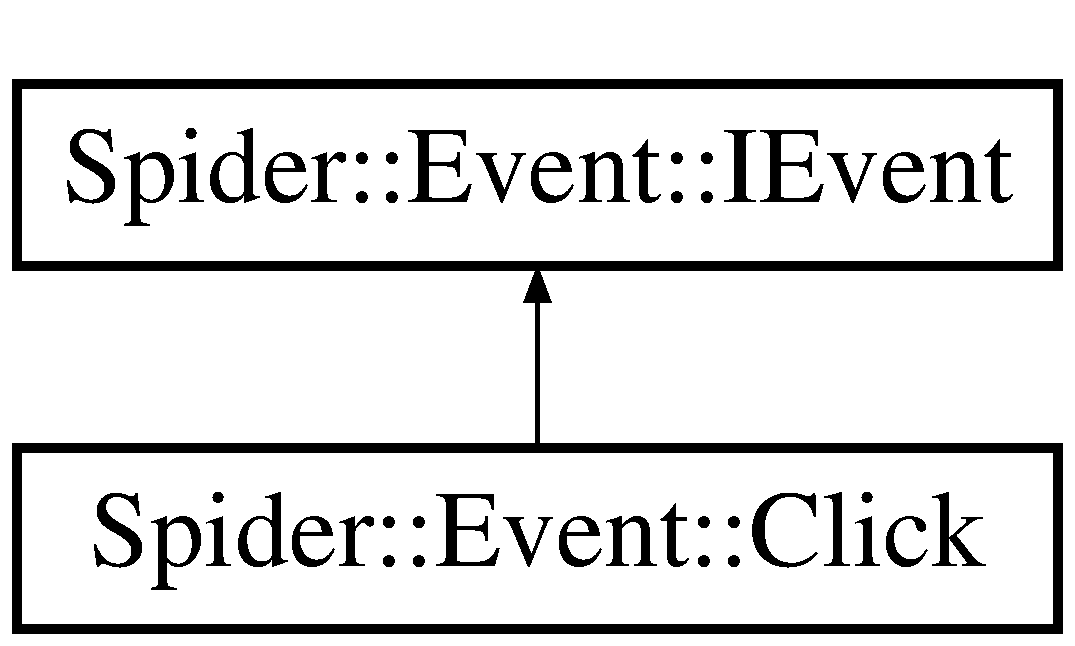
\includegraphics[height=2.000000cm]{class_spider_1_1_event_1_1_click}
\end{center}
\end{figure}
\subsection*{Public Member Functions}
\begin{DoxyCompactItemize}
\item 
\hyperlink{class_spider_1_1_event_1_1_click_a81c8bc490c33205c434b0c2e8db4b6f5}{Click} (\hyperlink{namespace_spider_1_1_event_ae178d39ebb8937d04ffe6ead8f306fd0}{Click\+Type} type, const std\+::string \&activity)
\begin{DoxyCompactList}\small\item\em Constructor with a Click\+Type. Save the mouse position. \end{DoxyCompactList}\item 
\mbox{\Hypertarget{class_spider_1_1_event_1_1_click_ac6170505ba14c87d8c8c83f9c9cc7000}\label{class_spider_1_1_event_1_1_click_ac6170505ba14c87d8c8c83f9c9cc7000}} 
\hyperlink{class_spider_1_1_event_1_1_click_ac6170505ba14c87d8c8c83f9c9cc7000}{Click} (const \hyperlink{class_spider_1_1_event_1_1_click}{Click} \&)=delete
\begin{DoxyCompactList}\small\item\em Default copy constructor. \end{DoxyCompactList}\item 
\hyperlink{class_spider_1_1_event_1_1_click}{Click} \& \hyperlink{class_spider_1_1_event_1_1_click_a857c3a0ca04ebce50cd170ec30e0a891}{operator=} (const \hyperlink{class_spider_1_1_event_1_1_click}{Click} \&)=delete
\begin{DoxyCompactList}\small\item\em Operator equal overlaod. \end{DoxyCompactList}\item 
\mbox{\Hypertarget{class_spider_1_1_event_1_1_click_a83a5ae5f70a0519d131a53c0a9b9c366}\label{class_spider_1_1_event_1_1_click_a83a5ae5f70a0519d131a53c0a9b9c366}} 
virtual \hyperlink{class_spider_1_1_event_1_1_click_a83a5ae5f70a0519d131a53c0a9b9c366}{$\sim$\+Click} ()=default
\begin{DoxyCompactList}\small\item\em Default destroyer. \end{DoxyCompactList}\item 
virtual std\+::string \hyperlink{class_spider_1_1_event_1_1_click_a916e746dc2145859f697de4d9f64cd00}{get\+Event\+Info} () const
\begin{DoxyCompactList}\small\item\em Extract \hyperlink{namespace_spider_1_1_event}{Event} information. \end{DoxyCompactList}\item 
virtual int \hyperlink{class_spider_1_1_event_1_1_click_a32b810199a69b799589b680bfb9c287d}{get\+Id} () const
\begin{DoxyCompactList}\small\item\em Get id of the event. \end{DoxyCompactList}\end{DoxyCompactItemize}
\subsection*{Additional Inherited Members}


\subsection{Constructor \& Destructor Documentation}
\mbox{\Hypertarget{class_spider_1_1_event_1_1_click_a81c8bc490c33205c434b0c2e8db4b6f5}\label{class_spider_1_1_event_1_1_click_a81c8bc490c33205c434b0c2e8db4b6f5}} 
\index{Spider\+::\+Event\+::\+Click@{Spider\+::\+Event\+::\+Click}!Click@{Click}}
\index{Click@{Click}!Spider\+::\+Event\+::\+Click@{Spider\+::\+Event\+::\+Click}}
\subsubsection{\texorpdfstring{Click()}{Click()}}
{\footnotesize\ttfamily Spider\+::\+Event\+::\+Click\+::\+Click (\begin{DoxyParamCaption}\item[{\hyperlink{namespace_spider_1_1_event_ae178d39ebb8937d04ffe6ead8f306fd0}{Click\+Type}}]{type,  }\item[{const std\+::string \&}]{activity }\end{DoxyParamCaption})}



Constructor with a Click\+Type. Save the mouse position. 


\begin{DoxyParams}{Parameters}
{\em type} & is the type of the click (left, middle or right) \\
\hline
{\em activity} & is the last activity register \\
\hline
\end{DoxyParams}


\subsection{Member Function Documentation}
\mbox{\Hypertarget{class_spider_1_1_event_1_1_click_a916e746dc2145859f697de4d9f64cd00}\label{class_spider_1_1_event_1_1_click_a916e746dc2145859f697de4d9f64cd00}} 
\index{Spider\+::\+Event\+::\+Click@{Spider\+::\+Event\+::\+Click}!get\+Event\+Info@{get\+Event\+Info}}
\index{get\+Event\+Info@{get\+Event\+Info}!Spider\+::\+Event\+::\+Click@{Spider\+::\+Event\+::\+Click}}
\subsubsection{\texorpdfstring{get\+Event\+Info()}{getEventInfo()}}
{\footnotesize\ttfamily virtual std\+::string Spider\+::\+Event\+::\+Click\+::get\+Event\+Info (\begin{DoxyParamCaption}{ }\end{DoxyParamCaption}) const\hspace{0.3cm}{\ttfamily [virtual]}}



Extract \hyperlink{namespace_spider_1_1_event}{Event} information. 

\begin{DoxyReturn}{Returns}
Informations into string format 
\end{DoxyReturn}


Implements \hyperlink{class_spider_1_1_event_1_1_i_event_ac8471df73080237faea55de539d968a0}{Spider\+::\+Event\+::\+I\+Event}.

\mbox{\Hypertarget{class_spider_1_1_event_1_1_click_a32b810199a69b799589b680bfb9c287d}\label{class_spider_1_1_event_1_1_click_a32b810199a69b799589b680bfb9c287d}} 
\index{Spider\+::\+Event\+::\+Click@{Spider\+::\+Event\+::\+Click}!get\+Id@{get\+Id}}
\index{get\+Id@{get\+Id}!Spider\+::\+Event\+::\+Click@{Spider\+::\+Event\+::\+Click}}
\subsubsection{\texorpdfstring{get\+Id()}{getId()}}
{\footnotesize\ttfamily virtual int Spider\+::\+Event\+::\+Click\+::get\+Id (\begin{DoxyParamCaption}{ }\end{DoxyParamCaption}) const\hspace{0.3cm}{\ttfamily [inline]}, {\ttfamily [virtual]}}



Get id of the event. 

\begin{DoxyReturn}{Returns}
\hyperlink{class_spider_1_1_event_1_1_request}{Request} ID 
\end{DoxyReturn}


Implements \hyperlink{class_spider_1_1_event_1_1_i_event_a902d1376faa8e5948fa5bfe8d7208c88}{Spider\+::\+Event\+::\+I\+Event}.

\mbox{\Hypertarget{class_spider_1_1_event_1_1_click_a857c3a0ca04ebce50cd170ec30e0a891}\label{class_spider_1_1_event_1_1_click_a857c3a0ca04ebce50cd170ec30e0a891}} 
\index{Spider\+::\+Event\+::\+Click@{Spider\+::\+Event\+::\+Click}!operator=@{operator=}}
\index{operator=@{operator=}!Spider\+::\+Event\+::\+Click@{Spider\+::\+Event\+::\+Click}}
\subsubsection{\texorpdfstring{operator=()}{operator=()}}
{\footnotesize\ttfamily \hyperlink{class_spider_1_1_event_1_1_click}{Click}\& Spider\+::\+Event\+::\+Click\+::operator= (\begin{DoxyParamCaption}\item[{const \hyperlink{class_spider_1_1_event_1_1_click}{Click} \&}]{ }\end{DoxyParamCaption})\hspace{0.3cm}{\ttfamily [delete]}}



Operator equal overlaod. 

\begin{DoxyReturn}{Returns}
\hyperlink{namespace_spider_1_1_event}{Event} interface 
\end{DoxyReturn}


The documentation for this class was generated from the following file\+:\begin{DoxyCompactItemize}
\item 
Event/Click.\+hpp\end{DoxyCompactItemize}

\hypertarget{class_c_lick}{}\section{C\+Lick Class Reference}
\label{class_c_lick}\index{C\+Lick@{C\+Lick}}


Handle click events.  




{\ttfamily \#include $<$Click.\+hpp$>$}



\subsection{Detailed Description}
Handle click events. 

The documentation for this class was generated from the following file\+:\begin{DoxyCompactItemize}
\item 
Event/Click.\+hpp\end{DoxyCompactItemize}

\hypertarget{struct_spider_1_1_event_1_1_click_coord}{}\section{Spider\+:\+:Event\+:\+:Click\+Coord Struct Reference}
\label{struct_spider_1_1_event_1_1_click_coord}\index{Spider\+::\+Event\+::\+Click\+Coord@{Spider\+::\+Event\+::\+Click\+Coord}}


Define the click coordonate.  




{\ttfamily \#include $<$I\+Event.\+hpp$>$}

\subsection*{Public Attributes}
\begin{DoxyCompactItemize}
\item 
\mbox{\Hypertarget{struct_spider_1_1_event_1_1_click_coord_a98b23924cdaa96ba6eacefbcec193d8f}\label{struct_spider_1_1_event_1_1_click_coord_a98b23924cdaa96ba6eacefbcec193d8f}} 
int {\bfseries pX}
\item 
\mbox{\Hypertarget{struct_spider_1_1_event_1_1_click_coord_ae64cc836b86d7ec976c93ca4e284ba8b}\label{struct_spider_1_1_event_1_1_click_coord_ae64cc836b86d7ec976c93ca4e284ba8b}} 
int {\bfseries pY}
\end{DoxyCompactItemize}


\subsection{Detailed Description}
Define the click coordonate. 

The documentation for this struct was generated from the following file\+:\begin{DoxyCompactItemize}
\item 
Event/\hyperlink{_i_event_8hpp}{I\+Event.\+hpp}\end{DoxyCompactItemize}

\hypertarget{classts_1_1common_1_1tcp_1_1_client_socket}{}\section{ts\+:\+:common\+:\+:tcp\+:\+:Client\+Socket Class Reference}
\label{classts_1_1common_1_1tcp_1_1_client_socket}\index{ts\+::common\+::tcp\+::\+Client\+Socket@{ts\+::common\+::tcp\+::\+Client\+Socket}}
\subsection*{Public Member Functions}
\begin{DoxyCompactItemize}
\item 
\mbox{\Hypertarget{classts_1_1common_1_1tcp_1_1_client_socket_a2d03e028676bd5f58db35c92ebe42029}\label{classts_1_1common_1_1tcp_1_1_client_socket_a2d03e028676bd5f58db35c92ebe42029}} 
{\bfseries Client\+Socket} (boost\+::asio\+::io\+\_\+service \&ios)
\item 
void \hyperlink{classts_1_1common_1_1tcp_1_1_client_socket_a0dda673c5f81c70c398c96a2a11ba152}{connect} (std\+::string const \&host, unsigned short port)
\item 
void \hyperlink{classts_1_1common_1_1tcp_1_1_client_socket_a6e852eb6629afd2fa253ccd3fd8a591a}{async\+Connect} (std\+::string const \&host, unsigned short port, On\+Connect\+Func on\+Connect)
\item 
void \hyperlink{classts_1_1common_1_1tcp_1_1_client_socket_a294447025579635cbfa7fe1829eb15a3}{close} ()
\item 
boost\+::asio\+::ip\+::tcp\+::socket \& \hyperlink{classts_1_1common_1_1tcp_1_1_client_socket_a951aaa6937d4acd0020d30aa8481a485}{get\+Socket} ()
\item 
bool \hyperlink{classts_1_1common_1_1tcp_1_1_client_socket_a654e7f9378b5143032c767486f1752f2}{is\+Connected} () const
\item 
size\+\_\+t \hyperlink{classts_1_1common_1_1tcp_1_1_client_socket_aa408490515485ebc5925685fa4cc4b93}{write} (void const $\ast$data, size\+\_\+t size)
\item 
void \hyperlink{classts_1_1common_1_1tcp_1_1_client_socket_acab3419c27934c50c8020b255af1a3ee}{async\+Write} (void const $\ast$data, size\+\_\+t size, On\+Write\+Func on\+Write=nullptr)
\item 
size\+\_\+t \hyperlink{classts_1_1common_1_1tcp_1_1_client_socket_a7876d2f81c6bf60f628973577dfabd2a}{read} (void $\ast$data, size\+\_\+t size)
\item 
void \hyperlink{classts_1_1common_1_1tcp_1_1_client_socket_afea6b565d0621b6d19648c0259b85e95}{async\+Read} (void $\ast$data, size\+\_\+t size, On\+Read\+Func on\+Read=nullptr)
\item 
void \hyperlink{classts_1_1common_1_1tcp_1_1_client_socket_a0fdc353f373b36eba7096ca88b957842}{set\+On\+Read\+Callback} (On\+Read\+Func on\+Read)
\item 
void \hyperlink{classts_1_1common_1_1tcp_1_1_client_socket_a6dc4758bd4b328dec0ee8cbc1a39820b}{set\+On\+Write\+Callback} (On\+Write\+Func on\+Write)
\item 
void \hyperlink{classts_1_1common_1_1tcp_1_1_client_socket_aeb8c00f0828b0d61c0f2a4b1aa486ff4}{set\+On\+Connect\+Callback} (On\+Connect\+Func on\+Connect)
\item 
\mbox{\Hypertarget{classts_1_1common_1_1tcp_1_1_client_socket_ae03a9e025ffc06eede204954a634a96e}\label{classts_1_1common_1_1tcp_1_1_client_socket_ae03a9e025ffc06eede204954a634a96e}} 
void {\bfseries set\+On\+Disconnect\+Callback} (On\+Disconnect on\+Disconnect)
\item 
std\+::string const  \& \hyperlink{classts_1_1common_1_1tcp_1_1_client_socket_a77d1bdcdd306a6487626ecbbdb4a0910}{get\+Address} ()
\item 
unsigned short \hyperlink{classts_1_1common_1_1tcp_1_1_client_socket_a3e17803779e94e89f3cda035a280d315}{get\+Port} ()
\item 
\mbox{\Hypertarget{classts_1_1common_1_1tcp_1_1_client_socket_a748fcc1565b851f1dd87dcf8c2d63057}\label{classts_1_1common_1_1tcp_1_1_client_socket_a748fcc1565b851f1dd87dcf8c2d63057}} 
void {\bfseries run} ()
\item 
\mbox{\Hypertarget{classts_1_1common_1_1tcp_1_1_client_socket_a7d1a90e4e2f918b899315a68cc3edd55}\label{classts_1_1common_1_1tcp_1_1_client_socket_a7d1a90e4e2f918b899315a68cc3edd55}} 
std\+::string {\bfseries get\+Info} ()
\item 
\mbox{\Hypertarget{classts_1_1common_1_1tcp_1_1_client_socket_aed2b9b1b3d589aaef9476df1f0800a6c}\label{classts_1_1common_1_1tcp_1_1_client_socket_aed2b9b1b3d589aaef9476df1f0800a6c}} 
void {\bfseries force\+Connection\+Status\+Has} (bool i)
\end{DoxyCompactItemize}
\subsection*{Protected Attributes}
\begin{DoxyCompactItemize}
\item 
\mbox{\Hypertarget{classts_1_1common_1_1tcp_1_1_client_socket_acb932dfbb7d1287af95c0f900563d8f7}\label{classts_1_1common_1_1tcp_1_1_client_socket_acb932dfbb7d1287af95c0f900563d8f7}} 
boost\+::asio\+::io\+\_\+service \& {\bfseries m\+Ios}
\item 
\mbox{\Hypertarget{classts_1_1common_1_1tcp_1_1_client_socket_a000d67633711815a8f2dc16acc9d2035}\label{classts_1_1common_1_1tcp_1_1_client_socket_a000d67633711815a8f2dc16acc9d2035}} 
boost\+::asio\+::ip\+::tcp\+::socket {\bfseries m\+Socket}
\item 
\mbox{\Hypertarget{classts_1_1common_1_1tcp_1_1_client_socket_aeede5987e5beb49f60c14840e84fd4eb}\label{classts_1_1common_1_1tcp_1_1_client_socket_aeede5987e5beb49f60c14840e84fd4eb}} 
bool {\bfseries m\+Is\+Connected}
\item 
\mbox{\Hypertarget{classts_1_1common_1_1tcp_1_1_client_socket_a5ebac0ae9230a9659b486d43a8b27b9b}\label{classts_1_1common_1_1tcp_1_1_client_socket_a5ebac0ae9230a9659b486d43a8b27b9b}} 
On\+Write\+Func {\bfseries m\+On\+Write}
\item 
\mbox{\Hypertarget{classts_1_1common_1_1tcp_1_1_client_socket_a116da217aaa9c4b18a6d7eb17994b58d}\label{classts_1_1common_1_1tcp_1_1_client_socket_a116da217aaa9c4b18a6d7eb17994b58d}} 
On\+Read\+Func {\bfseries m\+On\+Read}
\item 
\mbox{\Hypertarget{classts_1_1common_1_1tcp_1_1_client_socket_a79c7916f52cd6b18935200e042d55483}\label{classts_1_1common_1_1tcp_1_1_client_socket_a79c7916f52cd6b18935200e042d55483}} 
On\+Connect\+Func {\bfseries m\+On\+Connect}
\item 
\mbox{\Hypertarget{classts_1_1common_1_1tcp_1_1_client_socket_a3e19605ebf2eac6fe9d1b7c0e2c51fa1}\label{classts_1_1common_1_1tcp_1_1_client_socket_a3e19605ebf2eac6fe9d1b7c0e2c51fa1}} 
On\+Disconnect {\bfseries m\+On\+Disconnect}
\item 
\mbox{\Hypertarget{classts_1_1common_1_1tcp_1_1_client_socket_ad6ce1b1f3dfed87d9498610fcb75a5ef}\label{classts_1_1common_1_1tcp_1_1_client_socket_ad6ce1b1f3dfed87d9498610fcb75a5ef}} 
std\+::string {\bfseries m\+Address}
\item 
\mbox{\Hypertarget{classts_1_1common_1_1tcp_1_1_client_socket_a86914cea89264845b3e6f2b1213f48b5}\label{classts_1_1common_1_1tcp_1_1_client_socket_a86914cea89264845b3e6f2b1213f48b5}} 
unsigned short {\bfseries m\+Port}
\end{DoxyCompactItemize}


\subsection{Member Function Documentation}
\mbox{\Hypertarget{classts_1_1common_1_1tcp_1_1_client_socket_a6e852eb6629afd2fa253ccd3fd8a591a}\label{classts_1_1common_1_1tcp_1_1_client_socket_a6e852eb6629afd2fa253ccd3fd8a591a}} 
\index{ts\+::common\+::tcp\+::\+Client\+Socket@{ts\+::common\+::tcp\+::\+Client\+Socket}!async\+Connect@{async\+Connect}}
\index{async\+Connect@{async\+Connect}!ts\+::common\+::tcp\+::\+Client\+Socket@{ts\+::common\+::tcp\+::\+Client\+Socket}}
\subsubsection{\texorpdfstring{async\+Connect()}{asyncConnect()}}
{\footnotesize\ttfamily void ts\+::common\+::tcp\+::\+Client\+Socket\+::async\+Connect (\begin{DoxyParamCaption}\item[{std\+::string const \&}]{host,  }\item[{unsigned short}]{port,  }\item[{On\+Connect\+Func}]{on\+Connect }\end{DoxyParamCaption})}

Connect the client to the server asynchronously 
\begin{DoxyParams}{Parameters}
{\em host} & \\
\hline
{\em port} & \\
\hline
\end{DoxyParams}
\mbox{\Hypertarget{classts_1_1common_1_1tcp_1_1_client_socket_afea6b565d0621b6d19648c0259b85e95}\label{classts_1_1common_1_1tcp_1_1_client_socket_afea6b565d0621b6d19648c0259b85e95}} 
\index{ts\+::common\+::tcp\+::\+Client\+Socket@{ts\+::common\+::tcp\+::\+Client\+Socket}!async\+Read@{async\+Read}}
\index{async\+Read@{async\+Read}!ts\+::common\+::tcp\+::\+Client\+Socket@{ts\+::common\+::tcp\+::\+Client\+Socket}}
\subsubsection{\texorpdfstring{async\+Read()}{asyncRead()}}
{\footnotesize\ttfamily void ts\+::common\+::tcp\+::\+Client\+Socket\+::async\+Read (\begin{DoxyParamCaption}\item[{void $\ast$}]{data,  }\item[{size\+\_\+t}]{size,  }\item[{On\+Read\+Func}]{on\+Read = {\ttfamily nullptr} }\end{DoxyParamCaption})}

Read data asynchronously 
\begin{DoxyParams}{Parameters}
{\em data} & \\
\hline
{\em size} & \\
\hline
{\em on\+Read} & \\
\hline
\end{DoxyParams}
\mbox{\Hypertarget{classts_1_1common_1_1tcp_1_1_client_socket_acab3419c27934c50c8020b255af1a3ee}\label{classts_1_1common_1_1tcp_1_1_client_socket_acab3419c27934c50c8020b255af1a3ee}} 
\index{ts\+::common\+::tcp\+::\+Client\+Socket@{ts\+::common\+::tcp\+::\+Client\+Socket}!async\+Write@{async\+Write}}
\index{async\+Write@{async\+Write}!ts\+::common\+::tcp\+::\+Client\+Socket@{ts\+::common\+::tcp\+::\+Client\+Socket}}
\subsubsection{\texorpdfstring{async\+Write()}{asyncWrite()}}
{\footnotesize\ttfamily void ts\+::common\+::tcp\+::\+Client\+Socket\+::async\+Write (\begin{DoxyParamCaption}\item[{void const $\ast$}]{data,  }\item[{size\+\_\+t}]{size,  }\item[{On\+Write\+Func}]{on\+Write = {\ttfamily nullptr} }\end{DoxyParamCaption})}

Write data asynchronously 
\begin{DoxyParams}{Parameters}
{\em data} & \\
\hline
{\em size} & \\
\hline
{\em on\+Write} & \\
\hline
\end{DoxyParams}
\mbox{\Hypertarget{classts_1_1common_1_1tcp_1_1_client_socket_a294447025579635cbfa7fe1829eb15a3}\label{classts_1_1common_1_1tcp_1_1_client_socket_a294447025579635cbfa7fe1829eb15a3}} 
\index{ts\+::common\+::tcp\+::\+Client\+Socket@{ts\+::common\+::tcp\+::\+Client\+Socket}!close@{close}}
\index{close@{close}!ts\+::common\+::tcp\+::\+Client\+Socket@{ts\+::common\+::tcp\+::\+Client\+Socket}}
\subsubsection{\texorpdfstring{close()}{close()}}
{\footnotesize\ttfamily void ts\+::common\+::tcp\+::\+Client\+Socket\+::close (\begin{DoxyParamCaption}{ }\end{DoxyParamCaption})}

Close the Client connection \mbox{\Hypertarget{classts_1_1common_1_1tcp_1_1_client_socket_a0dda673c5f81c70c398c96a2a11ba152}\label{classts_1_1common_1_1tcp_1_1_client_socket_a0dda673c5f81c70c398c96a2a11ba152}} 
\index{ts\+::common\+::tcp\+::\+Client\+Socket@{ts\+::common\+::tcp\+::\+Client\+Socket}!connect@{connect}}
\index{connect@{connect}!ts\+::common\+::tcp\+::\+Client\+Socket@{ts\+::common\+::tcp\+::\+Client\+Socket}}
\subsubsection{\texorpdfstring{connect()}{connect()}}
{\footnotesize\ttfamily void ts\+::common\+::tcp\+::\+Client\+Socket\+::connect (\begin{DoxyParamCaption}\item[{std\+::string const \&}]{host,  }\item[{unsigned short}]{port }\end{DoxyParamCaption})}

Connect the client to the server 
\begin{DoxyParams}{Parameters}
{\em host} & \\
\hline
{\em port} & \\
\hline
\end{DoxyParams}
\mbox{\Hypertarget{classts_1_1common_1_1tcp_1_1_client_socket_a77d1bdcdd306a6487626ecbbdb4a0910}\label{classts_1_1common_1_1tcp_1_1_client_socket_a77d1bdcdd306a6487626ecbbdb4a0910}} 
\index{ts\+::common\+::tcp\+::\+Client\+Socket@{ts\+::common\+::tcp\+::\+Client\+Socket}!get\+Address@{get\+Address}}
\index{get\+Address@{get\+Address}!ts\+::common\+::tcp\+::\+Client\+Socket@{ts\+::common\+::tcp\+::\+Client\+Socket}}
\subsubsection{\texorpdfstring{get\+Address()}{getAddress()}}
{\footnotesize\ttfamily std\+::string const\& ts\+::common\+::tcp\+::\+Client\+Socket\+::get\+Address (\begin{DoxyParamCaption}{ }\end{DoxyParamCaption})}

Return the address \begin{DoxyReturn}{Returns}

\end{DoxyReturn}
\mbox{\Hypertarget{classts_1_1common_1_1tcp_1_1_client_socket_a3e17803779e94e89f3cda035a280d315}\label{classts_1_1common_1_1tcp_1_1_client_socket_a3e17803779e94e89f3cda035a280d315}} 
\index{ts\+::common\+::tcp\+::\+Client\+Socket@{ts\+::common\+::tcp\+::\+Client\+Socket}!get\+Port@{get\+Port}}
\index{get\+Port@{get\+Port}!ts\+::common\+::tcp\+::\+Client\+Socket@{ts\+::common\+::tcp\+::\+Client\+Socket}}
\subsubsection{\texorpdfstring{get\+Port()}{getPort()}}
{\footnotesize\ttfamily unsigned short ts\+::common\+::tcp\+::\+Client\+Socket\+::get\+Port (\begin{DoxyParamCaption}{ }\end{DoxyParamCaption})}

Return the port \begin{DoxyReturn}{Returns}

\end{DoxyReturn}
\mbox{\Hypertarget{classts_1_1common_1_1tcp_1_1_client_socket_a951aaa6937d4acd0020d30aa8481a485}\label{classts_1_1common_1_1tcp_1_1_client_socket_a951aaa6937d4acd0020d30aa8481a485}} 
\index{ts\+::common\+::tcp\+::\+Client\+Socket@{ts\+::common\+::tcp\+::\+Client\+Socket}!get\+Socket@{get\+Socket}}
\index{get\+Socket@{get\+Socket}!ts\+::common\+::tcp\+::\+Client\+Socket@{ts\+::common\+::tcp\+::\+Client\+Socket}}
\subsubsection{\texorpdfstring{get\+Socket()}{getSocket()}}
{\footnotesize\ttfamily boost\+::asio\+::ip\+::tcp\+::socket\& ts\+::common\+::tcp\+::\+Client\+Socket\+::get\+Socket (\begin{DoxyParamCaption}{ }\end{DoxyParamCaption})}

Return the Boost asio socket \begin{DoxyReturn}{Returns}

\end{DoxyReturn}
\mbox{\Hypertarget{classts_1_1common_1_1tcp_1_1_client_socket_a654e7f9378b5143032c767486f1752f2}\label{classts_1_1common_1_1tcp_1_1_client_socket_a654e7f9378b5143032c767486f1752f2}} 
\index{ts\+::common\+::tcp\+::\+Client\+Socket@{ts\+::common\+::tcp\+::\+Client\+Socket}!is\+Connected@{is\+Connected}}
\index{is\+Connected@{is\+Connected}!ts\+::common\+::tcp\+::\+Client\+Socket@{ts\+::common\+::tcp\+::\+Client\+Socket}}
\subsubsection{\texorpdfstring{is\+Connected()}{isConnected()}}
{\footnotesize\ttfamily bool ts\+::common\+::tcp\+::\+Client\+Socket\+::is\+Connected (\begin{DoxyParamCaption}{ }\end{DoxyParamCaption}) const}

Check if the client is connect the server \begin{DoxyReturn}{Returns}

\end{DoxyReturn}
\mbox{\Hypertarget{classts_1_1common_1_1tcp_1_1_client_socket_a7876d2f81c6bf60f628973577dfabd2a}\label{classts_1_1common_1_1tcp_1_1_client_socket_a7876d2f81c6bf60f628973577dfabd2a}} 
\index{ts\+::common\+::tcp\+::\+Client\+Socket@{ts\+::common\+::tcp\+::\+Client\+Socket}!read@{read}}
\index{read@{read}!ts\+::common\+::tcp\+::\+Client\+Socket@{ts\+::common\+::tcp\+::\+Client\+Socket}}
\subsubsection{\texorpdfstring{read()}{read()}}
{\footnotesize\ttfamily size\+\_\+t ts\+::common\+::tcp\+::\+Client\+Socket\+::read (\begin{DoxyParamCaption}\item[{void $\ast$}]{data,  }\item[{size\+\_\+t}]{size }\end{DoxyParamCaption})}

Read data 
\begin{DoxyParams}{Parameters}
{\em data} & \\
\hline
{\em size} & \\
\hline
\end{DoxyParams}
\begin{DoxyReturn}{Returns}

\end{DoxyReturn}
\mbox{\Hypertarget{classts_1_1common_1_1tcp_1_1_client_socket_aeb8c00f0828b0d61c0f2a4b1aa486ff4}\label{classts_1_1common_1_1tcp_1_1_client_socket_aeb8c00f0828b0d61c0f2a4b1aa486ff4}} 
\index{ts\+::common\+::tcp\+::\+Client\+Socket@{ts\+::common\+::tcp\+::\+Client\+Socket}!set\+On\+Connect\+Callback@{set\+On\+Connect\+Callback}}
\index{set\+On\+Connect\+Callback@{set\+On\+Connect\+Callback}!ts\+::common\+::tcp\+::\+Client\+Socket@{ts\+::common\+::tcp\+::\+Client\+Socket}}
\subsubsection{\texorpdfstring{set\+On\+Connect\+Callback()}{setOnConnectCallback()}}
{\footnotesize\ttfamily void ts\+::common\+::tcp\+::\+Client\+Socket\+::set\+On\+Connect\+Callback (\begin{DoxyParamCaption}\item[{On\+Connect\+Func}]{on\+Connect }\end{DoxyParamCaption})}

Set the callback for async\+Connect \begin{DoxySeeAlso}{See also}
\hyperlink{classts_1_1common_1_1tcp_1_1_client_socket_a6e852eb6629afd2fa253ccd3fd8a591a}{async\+Connect} 
\end{DoxySeeAlso}

\begin{DoxyParams}{Parameters}
{\em on\+Connect} & \\
\hline
\end{DoxyParams}
\mbox{\Hypertarget{classts_1_1common_1_1tcp_1_1_client_socket_a0fdc353f373b36eba7096ca88b957842}\label{classts_1_1common_1_1tcp_1_1_client_socket_a0fdc353f373b36eba7096ca88b957842}} 
\index{ts\+::common\+::tcp\+::\+Client\+Socket@{ts\+::common\+::tcp\+::\+Client\+Socket}!set\+On\+Read\+Callback@{set\+On\+Read\+Callback}}
\index{set\+On\+Read\+Callback@{set\+On\+Read\+Callback}!ts\+::common\+::tcp\+::\+Client\+Socket@{ts\+::common\+::tcp\+::\+Client\+Socket}}
\subsubsection{\texorpdfstring{set\+On\+Read\+Callback()}{setOnReadCallback()}}
{\footnotesize\ttfamily void ts\+::common\+::tcp\+::\+Client\+Socket\+::set\+On\+Read\+Callback (\begin{DoxyParamCaption}\item[{On\+Read\+Func}]{on\+Read }\end{DoxyParamCaption})}

Set the callback for async\+Read \begin{DoxySeeAlso}{See also}
\hyperlink{classts_1_1common_1_1tcp_1_1_client_socket_afea6b565d0621b6d19648c0259b85e95}{async\+Read} 
\end{DoxySeeAlso}

\begin{DoxyParams}{Parameters}
{\em on\+Read} & \\
\hline
\end{DoxyParams}
\mbox{\Hypertarget{classts_1_1common_1_1tcp_1_1_client_socket_a6dc4758bd4b328dec0ee8cbc1a39820b}\label{classts_1_1common_1_1tcp_1_1_client_socket_a6dc4758bd4b328dec0ee8cbc1a39820b}} 
\index{ts\+::common\+::tcp\+::\+Client\+Socket@{ts\+::common\+::tcp\+::\+Client\+Socket}!set\+On\+Write\+Callback@{set\+On\+Write\+Callback}}
\index{set\+On\+Write\+Callback@{set\+On\+Write\+Callback}!ts\+::common\+::tcp\+::\+Client\+Socket@{ts\+::common\+::tcp\+::\+Client\+Socket}}
\subsubsection{\texorpdfstring{set\+On\+Write\+Callback()}{setOnWriteCallback()}}
{\footnotesize\ttfamily void ts\+::common\+::tcp\+::\+Client\+Socket\+::set\+On\+Write\+Callback (\begin{DoxyParamCaption}\item[{On\+Write\+Func}]{on\+Write }\end{DoxyParamCaption})}

Set the callback for async\+Write \begin{DoxySeeAlso}{See also}
\hyperlink{classts_1_1common_1_1tcp_1_1_client_socket_acab3419c27934c50c8020b255af1a3ee}{async\+Write} 
\end{DoxySeeAlso}

\begin{DoxyParams}{Parameters}
{\em on\+Write} & \\
\hline
\end{DoxyParams}
\mbox{\Hypertarget{classts_1_1common_1_1tcp_1_1_client_socket_aa408490515485ebc5925685fa4cc4b93}\label{classts_1_1common_1_1tcp_1_1_client_socket_aa408490515485ebc5925685fa4cc4b93}} 
\index{ts\+::common\+::tcp\+::\+Client\+Socket@{ts\+::common\+::tcp\+::\+Client\+Socket}!write@{write}}
\index{write@{write}!ts\+::common\+::tcp\+::\+Client\+Socket@{ts\+::common\+::tcp\+::\+Client\+Socket}}
\subsubsection{\texorpdfstring{write()}{write()}}
{\footnotesize\ttfamily size\+\_\+t ts\+::common\+::tcp\+::\+Client\+Socket\+::write (\begin{DoxyParamCaption}\item[{void const $\ast$}]{data,  }\item[{size\+\_\+t}]{size }\end{DoxyParamCaption})}

Write data 
\begin{DoxyParams}{Parameters}
{\em data} & \\
\hline
{\em size} & \\
\hline
\end{DoxyParams}
\begin{DoxyReturn}{Returns}

\end{DoxyReturn}


The documentation for this class was generated from the following file\+:\begin{DoxyCompactItemize}
\item 
Socket/Tcp\+Client\+Socket.\+hpp\end{DoxyCompactItemize}

\hypertarget{class_spider_1_1_core_exception}{}\section{Spider\+:\+:Core\+Exception Class Reference}
\label{class_spider_1_1_core_exception}\index{Spider\+::\+Core\+Exception@{Spider\+::\+Core\+Exception}}


Core exception class.  




{\ttfamily \#include $<$Core\+Exception.\+hpp$>$}

Inheritance diagram for Spider\+:\+:Core\+Exception\+:\begin{figure}[H]
\begin{center}
\leavevmode
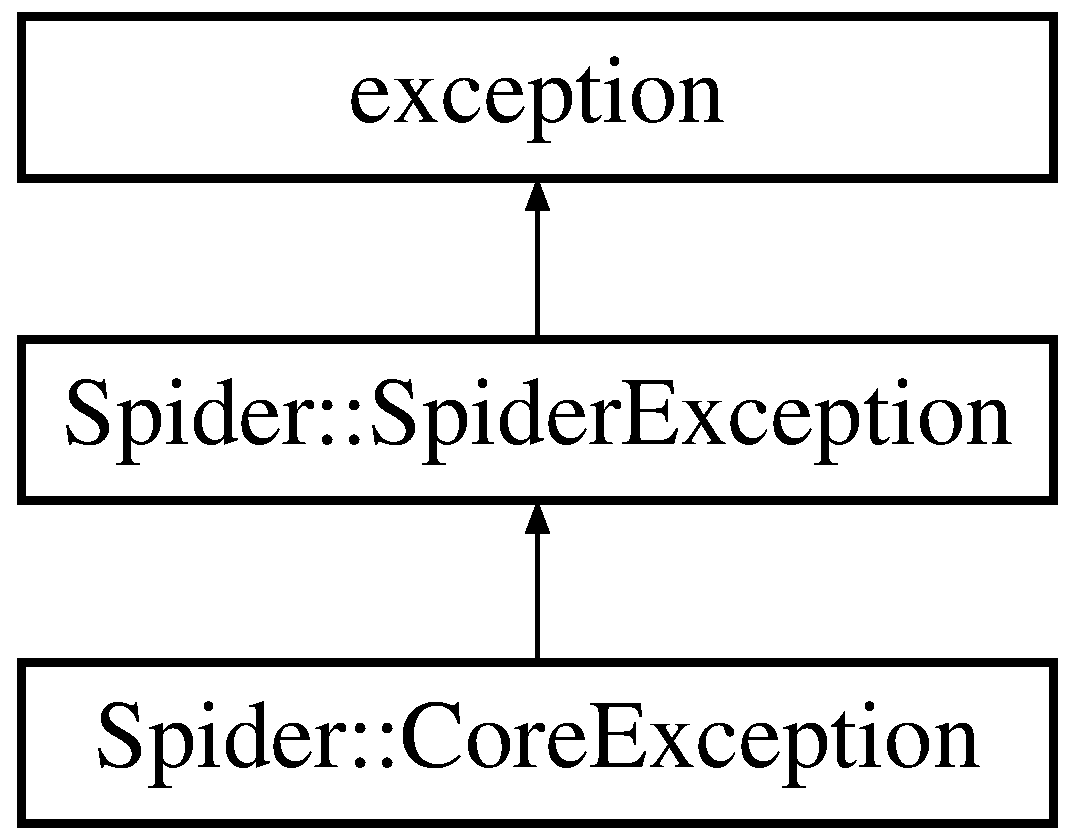
\includegraphics[height=3.000000cm]{class_spider_1_1_core_exception}
\end{center}
\end{figure}
\subsection*{Public Member Functions}
\begin{DoxyCompactItemize}
\item 
\hyperlink{class_spider_1_1_core_exception_a097cb8e36be15a4ee1527e7a32039da1}{Core\+Exception} (const std\+::string \&msg)
\begin{DoxyCompactList}\small\item\em Constructor of the default \hyperlink{class_spider_1_1_core_exception}{Core\+Exception} class. \end{DoxyCompactList}\item 
\mbox{\Hypertarget{class_spider_1_1_core_exception_a350c0791fec090676c3630b5f4de6f27}\label{class_spider_1_1_core_exception_a350c0791fec090676c3630b5f4de6f27}} 
virtual \hyperlink{class_spider_1_1_core_exception_a350c0791fec090676c3630b5f4de6f27}{$\sim$\+Core\+Exception} ()  throw ()
\begin{DoxyCompactList}\small\item\em Destructor of class \hyperlink{class_spider_1_1_core_exception}{Core\+Exception}. \end{DoxyCompactList}\end{DoxyCompactItemize}


\subsection{Detailed Description}
Core exception class. 

\subsection{Constructor \& Destructor Documentation}
\mbox{\Hypertarget{class_spider_1_1_core_exception_a097cb8e36be15a4ee1527e7a32039da1}\label{class_spider_1_1_core_exception_a097cb8e36be15a4ee1527e7a32039da1}} 
\index{Spider\+::\+Core\+Exception@{Spider\+::\+Core\+Exception}!Core\+Exception@{Core\+Exception}}
\index{Core\+Exception@{Core\+Exception}!Spider\+::\+Core\+Exception@{Spider\+::\+Core\+Exception}}
\subsubsection{\texorpdfstring{Core\+Exception()}{CoreException()}}
{\footnotesize\ttfamily Spider\+::\+Core\+Exception\+::\+Core\+Exception (\begin{DoxyParamCaption}\item[{const std\+::string \&}]{msg }\end{DoxyParamCaption})\hspace{0.3cm}{\ttfamily [inline]}}



Constructor of the default \hyperlink{class_spider_1_1_core_exception}{Core\+Exception} class. 


\begin{DoxyParams}{Parameters}
{\em msg} & Message related to the exception sent \\
\hline
\end{DoxyParams}


The documentation for this class was generated from the following file\+:\begin{DoxyCompactItemize}
\item 
Exception/\hyperlink{_core_exception_8hpp}{Core\+Exception.\+hpp}\end{DoxyCompactItemize}

\hypertarget{class_spider_1_1_d_b_exception}{}\section{Spider\+:\+:D\+B\+Exception Class Reference}
\label{class_spider_1_1_d_b_exception}\index{Spider\+::\+D\+B\+Exception@{Spider\+::\+D\+B\+Exception}}
Inheritance diagram for Spider\+:\+:D\+B\+Exception\+:\begin{figure}[H]
\begin{center}
\leavevmode
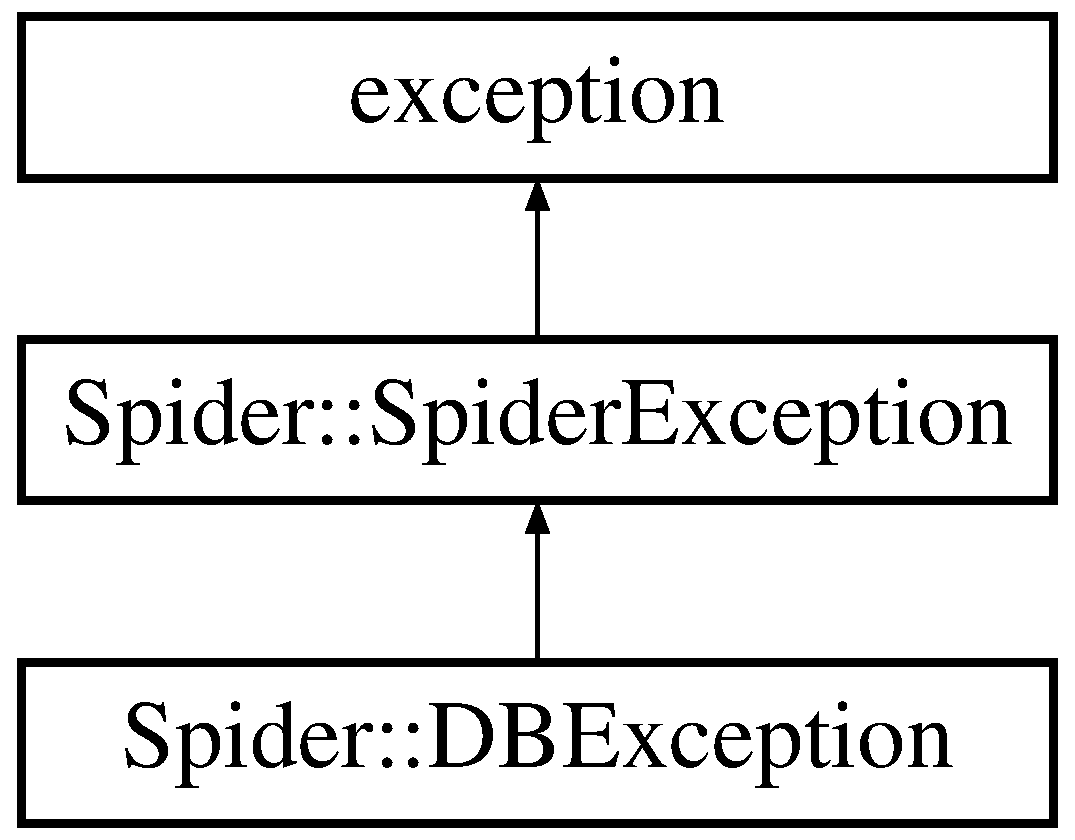
\includegraphics[height=3.000000cm]{class_spider_1_1_d_b_exception}
\end{center}
\end{figure}
\subsection*{Public Member Functions}
\begin{DoxyCompactItemize}
\item 
\hyperlink{class_spider_1_1_d_b_exception_a3f256a7e5b01d9d68b9d65305868aa29}{D\+B\+Exception} (const std\+::string \&msg)
\begin{DoxyCompactList}\small\item\em Constructor of the default \hyperlink{class_spider_1_1_d_b_exception}{D\+B\+Exception} class. \end{DoxyCompactList}\item 
\mbox{\Hypertarget{class_spider_1_1_d_b_exception_ace8f79b6896a3bb356ca254ad9116190}\label{class_spider_1_1_d_b_exception_ace8f79b6896a3bb356ca254ad9116190}} 
virtual \hyperlink{class_spider_1_1_d_b_exception_ace8f79b6896a3bb356ca254ad9116190}{$\sim$\+D\+B\+Exception} ()  throw ()
\begin{DoxyCompactList}\small\item\em Destructor of class \hyperlink{class_spider_1_1_d_b_exception}{D\+B\+Exception}. \end{DoxyCompactList}\end{DoxyCompactItemize}


\subsection{Constructor \& Destructor Documentation}
\mbox{\Hypertarget{class_spider_1_1_d_b_exception_a3f256a7e5b01d9d68b9d65305868aa29}\label{class_spider_1_1_d_b_exception_a3f256a7e5b01d9d68b9d65305868aa29}} 
\index{Spider\+::\+D\+B\+Exception@{Spider\+::\+D\+B\+Exception}!D\+B\+Exception@{D\+B\+Exception}}
\index{D\+B\+Exception@{D\+B\+Exception}!Spider\+::\+D\+B\+Exception@{Spider\+::\+D\+B\+Exception}}
\subsubsection{\texorpdfstring{D\+B\+Exception()}{DBException()}}
{\footnotesize\ttfamily Spider\+::\+D\+B\+Exception\+::\+D\+B\+Exception (\begin{DoxyParamCaption}\item[{const std\+::string \&}]{msg }\end{DoxyParamCaption})\hspace{0.3cm}{\ttfamily [inline]}}



Constructor of the default \hyperlink{class_spider_1_1_d_b_exception}{D\+B\+Exception} class. 


\begin{DoxyParams}{Parameters}
{\em msg} & Message related to the exception sent \\
\hline
\end{DoxyParams}


The documentation for this class was generated from the following file\+:\begin{DoxyCompactItemize}
\item 
Exception/\hyperlink{_d_b_exception_8hpp}{D\+B\+Exception.\+hpp}\end{DoxyCompactItemize}

\hypertarget{class_spider_1_1_d_b_1_1_d_b_handler}{}\section{Spider\+:\+:DB\+:\+:D\+B\+Handler Class Reference}
\label{class_spider_1_1_d_b_1_1_d_b_handler}\index{Spider\+::\+D\+B\+::\+D\+B\+Handler@{Spider\+::\+D\+B\+::\+D\+B\+Handler}}
\subsection*{Public Member Functions}
\begin{DoxyCompactItemize}
\item 
\mbox{\Hypertarget{class_spider_1_1_d_b_1_1_d_b_handler_a0f7f1767a084f374feb6ce414adde9c9}\label{class_spider_1_1_d_b_1_1_d_b_handler_a0f7f1767a084f374feb6ce414adde9c9}} 
\hyperlink{class_spider_1_1_d_b_1_1_d_b_handler_a0f7f1767a084f374feb6ce414adde9c9}{D\+B\+Handler} ()
\begin{DoxyCompactList}\small\item\em Default \hyperlink{class_spider_1_1_d_b_1_1_d_b_handler}{D\+B\+Handler} constructor. \end{DoxyCompactList}\item 
\mbox{\Hypertarget{class_spider_1_1_d_b_1_1_d_b_handler_a72a1ba5dbf9777dfb094e295bc9f08a4}\label{class_spider_1_1_d_b_1_1_d_b_handler_a72a1ba5dbf9777dfb094e295bc9f08a4}} 
\hyperlink{class_spider_1_1_d_b_1_1_d_b_handler_a72a1ba5dbf9777dfb094e295bc9f08a4}{D\+B\+Handler} (const \hyperlink{class_spider_1_1_d_b_1_1_d_b_handler}{D\+B\+Handler} \&)=delete
\begin{DoxyCompactList}\small\item\em Default copy constructor. \end{DoxyCompactList}\item 
\mbox{\Hypertarget{class_spider_1_1_d_b_1_1_d_b_handler_a8f507845f01a1af5c83a5535e0529442}\label{class_spider_1_1_d_b_1_1_d_b_handler_a8f507845f01a1af5c83a5535e0529442}} 
\hyperlink{class_spider_1_1_d_b_1_1_d_b_handler}{D\+B\+Handler} \& \hyperlink{class_spider_1_1_d_b_1_1_d_b_handler_a8f507845f01a1af5c83a5535e0529442}{operator=} (const \hyperlink{class_spider_1_1_d_b_1_1_d_b_handler}{D\+B\+Handler} \&)=delete
\begin{DoxyCompactList}\small\item\em Equal operator overload. \end{DoxyCompactList}\item 
\mbox{\Hypertarget{class_spider_1_1_d_b_1_1_d_b_handler_a86700944ee698f784de64c20e5bb6f86}\label{class_spider_1_1_d_b_1_1_d_b_handler_a86700944ee698f784de64c20e5bb6f86}} 
\hyperlink{class_spider_1_1_d_b_1_1_d_b_handler_a86700944ee698f784de64c20e5bb6f86}{$\sim$\+D\+B\+Handler} ()=default
\begin{DoxyCompactList}\small\item\em Default destructor. \end{DoxyCompactList}\item 
void \hyperlink{class_spider_1_1_d_b_1_1_d_b_handler_a139355686a0f6eca4b58d26332c9a5c7}{connect} (const std\+::string \&name)
\begin{DoxyCompactList}\small\item\em Connect fonction, create a data base. \end{DoxyCompactList}\item 
\mbox{\Hypertarget{class_spider_1_1_d_b_1_1_d_b_handler_af3c0ca362f8aa317a199d97d578d2506}\label{class_spider_1_1_d_b_1_1_d_b_handler_af3c0ca362f8aa317a199d97d578d2506}} 
void \hyperlink{class_spider_1_1_d_b_1_1_d_b_handler_af3c0ca362f8aa317a199d97d578d2506}{disconnect} ()
\begin{DoxyCompactList}\small\item\em Disconnect the instance of data base previously create. \end{DoxyCompactList}\item 
void \hyperlink{class_spider_1_1_d_b_1_1_d_b_handler_a12968ed2952aa4365d17733227bc4cdb}{push} (const \hyperlink{class_spider_1_1_event_1_1_request}{Event\+::\+Request} \&request)
\begin{DoxyCompactList}\small\item\em Push a request in the data base. \end{DoxyCompactList}\item 
\mbox{\Hypertarget{class_spider_1_1_d_b_1_1_d_b_handler_a76b1ef1bd0463caded154fd1400445f9}\label{class_spider_1_1_d_b_1_1_d_b_handler_a76b1ef1bd0463caded154fd1400445f9}} 
void \hyperlink{class_spider_1_1_d_b_1_1_d_b_handler_a76b1ef1bd0463caded154fd1400445f9}{pop} ()
\begin{DoxyCompactList}\small\item\em delete the last element of the data base \end{DoxyCompactList}\item 
\mbox{\Hypertarget{class_spider_1_1_d_b_1_1_d_b_handler_ac518baf148ad74676cdcfd3d16d57263}\label{class_spider_1_1_d_b_1_1_d_b_handler_ac518baf148ad74676cdcfd3d16d57263}} 
void \hyperlink{class_spider_1_1_d_b_1_1_d_b_handler_ac518baf148ad74676cdcfd3d16d57263}{delete\+Table} ()
\begin{DoxyCompactList}\small\item\em Delete the spider table from the data base. \end{DoxyCompactList}\item 
\mbox{\Hypertarget{class_spider_1_1_d_b_1_1_d_b_handler_a3068d47caf9cb45d72f3cd99530364f1}\label{class_spider_1_1_d_b_1_1_d_b_handler_a3068d47caf9cb45d72f3cd99530364f1}} 
void \hyperlink{class_spider_1_1_d_b_1_1_d_b_handler_a3068d47caf9cb45d72f3cd99530364f1}{show\+Table} ()
\begin{DoxyCompactList}\small\item\em Show all informations from the data base. \end{DoxyCompactList}\end{DoxyCompactItemize}


\subsection{Member Function Documentation}
\mbox{\Hypertarget{class_spider_1_1_d_b_1_1_d_b_handler_a139355686a0f6eca4b58d26332c9a5c7}\label{class_spider_1_1_d_b_1_1_d_b_handler_a139355686a0f6eca4b58d26332c9a5c7}} 
\index{Spider\+::\+D\+B\+::\+D\+B\+Handler@{Spider\+::\+D\+B\+::\+D\+B\+Handler}!connect@{connect}}
\index{connect@{connect}!Spider\+::\+D\+B\+::\+D\+B\+Handler@{Spider\+::\+D\+B\+::\+D\+B\+Handler}}
\subsubsection{\texorpdfstring{connect()}{connect()}}
{\footnotesize\ttfamily void Spider\+::\+D\+B\+::\+D\+B\+Handler\+::connect (\begin{DoxyParamCaption}\item[{const std\+::string \&}]{name }\end{DoxyParamCaption})}



Connect fonction, create a data base. 


\begin{DoxyParams}{Parameters}
{\em name} & The name of the futur data base \\
\hline
\end{DoxyParams}
\mbox{\Hypertarget{class_spider_1_1_d_b_1_1_d_b_handler_a12968ed2952aa4365d17733227bc4cdb}\label{class_spider_1_1_d_b_1_1_d_b_handler_a12968ed2952aa4365d17733227bc4cdb}} 
\index{Spider\+::\+D\+B\+::\+D\+B\+Handler@{Spider\+::\+D\+B\+::\+D\+B\+Handler}!push@{push}}
\index{push@{push}!Spider\+::\+D\+B\+::\+D\+B\+Handler@{Spider\+::\+D\+B\+::\+D\+B\+Handler}}
\subsubsection{\texorpdfstring{push()}{push()}}
{\footnotesize\ttfamily void Spider\+::\+D\+B\+::\+D\+B\+Handler\+::push (\begin{DoxyParamCaption}\item[{const \hyperlink{class_spider_1_1_event_1_1_request}{Event\+::\+Request} \&}]{request }\end{DoxyParamCaption})}



Push a request in the data base. 


\begin{DoxyParams}{Parameters}
{\em request} & Request to push on the data base \\
\hline
\end{DoxyParams}


The documentation for this class was generated from the following file\+:\begin{DoxyCompactItemize}
\item 
D\+B/\hyperlink{_d_b_handler_8hpp}{D\+B\+Handler.\+hpp}\end{DoxyCompactItemize}

\hypertarget{class_spider_1_1_event_1_1_event_handler}{}\section{Spider\+:\+:Event\+:\+:Event\+Handler Class Reference}
\label{class_spider_1_1_event_1_1_event_handler}\index{Spider\+::\+Event\+::\+Event\+Handler@{Spider\+::\+Event\+::\+Event\+Handler}}


Handle events.  




{\ttfamily \#include $<$Event\+Handler.\+hpp$>$}

\subsection*{Public Member Functions}
\begin{DoxyCompactItemize}
\item 
\hyperlink{class_spider_1_1_event_1_1_event_handler_a97d86b6085e4158f8389f2e31dd0c336}{Event\+Handler} (const std\+::string \&host, unsigned short port)
\begin{DoxyCompactList}\small\item\em Default constructor. \end{DoxyCompactList}\item 
\mbox{\Hypertarget{class_spider_1_1_event_1_1_event_handler_a3c8af183af0a7e88983cea02883bc674}\label{class_spider_1_1_event_1_1_event_handler_a3c8af183af0a7e88983cea02883bc674}} 
\hyperlink{class_spider_1_1_event_1_1_event_handler_a3c8af183af0a7e88983cea02883bc674}{Event\+Handler} (const \hyperlink{class_spider_1_1_event_1_1_event_handler}{Event\+Handler} \&handler)=delete
\begin{DoxyCompactList}\small\item\em Default copy constructor. \end{DoxyCompactList}\item 
\mbox{\Hypertarget{class_spider_1_1_event_1_1_event_handler_a1b6435063e41baebcf95e0d30962b05a}\label{class_spider_1_1_event_1_1_event_handler_a1b6435063e41baebcf95e0d30962b05a}} 
\hyperlink{class_spider_1_1_event_1_1_event_handler}{Event\+Handler} \& \hyperlink{class_spider_1_1_event_1_1_event_handler_a1b6435063e41baebcf95e0d30962b05a}{operator=} (const \hyperlink{class_spider_1_1_event_1_1_event_handler}{Event\+Handler} \&handler)=delete
\begin{DoxyCompactList}\small\item\em Equal operator overload. \end{DoxyCompactList}\item 
\mbox{\Hypertarget{class_spider_1_1_event_1_1_event_handler_a114b675a93ef37e4f32cd264c210bf27}\label{class_spider_1_1_event_1_1_event_handler_a114b675a93ef37e4f32cd264c210bf27}} 
\hyperlink{class_spider_1_1_event_1_1_event_handler_a114b675a93ef37e4f32cd264c210bf27}{$\sim$\+Event\+Handler} ()
\begin{DoxyCompactList}\small\item\em Default destructor. \end{DoxyCompactList}\item 
bool \hyperlink{class_spider_1_1_event_1_1_event_handler_a09a8b1b3bfce070dc83226db55c7664f}{handle} (const std\+::shared\+\_\+ptr$<$ \hyperlink{class_spider_1_1_event_1_1_i_event}{I\+Event} $>$ \&event, const \hyperlink{class_spider_1_1ssl_1_1_r_s_a_keys}{ssl\+::\+R\+S\+A\+Keys} \&rsa)
\begin{DoxyCompactList}\small\item\em Handle a event. \end{DoxyCompactList}\end{DoxyCompactItemize}


\subsection{Detailed Description}
Handle events. 

\subsection{Constructor \& Destructor Documentation}
\mbox{\Hypertarget{class_spider_1_1_event_1_1_event_handler_a97d86b6085e4158f8389f2e31dd0c336}\label{class_spider_1_1_event_1_1_event_handler_a97d86b6085e4158f8389f2e31dd0c336}} 
\index{Spider\+::\+Event\+::\+Event\+Handler@{Spider\+::\+Event\+::\+Event\+Handler}!Event\+Handler@{Event\+Handler}}
\index{Event\+Handler@{Event\+Handler}!Spider\+::\+Event\+::\+Event\+Handler@{Spider\+::\+Event\+::\+Event\+Handler}}
\subsubsection{\texorpdfstring{Event\+Handler()}{EventHandler()}}
{\footnotesize\ttfamily Spider\+::\+Event\+::\+Event\+Handler\+::\+Event\+Handler (\begin{DoxyParamCaption}\item[{const std\+::string \&}]{host,  }\item[{unsigned short}]{port }\end{DoxyParamCaption})}



Default constructor. 


\begin{DoxyParams}{Parameters}
{\em host} & Host to connect \\
\hline
{\em port} & Port of the host \\
\hline
\end{DoxyParams}


\subsection{Member Function Documentation}
\mbox{\Hypertarget{class_spider_1_1_event_1_1_event_handler_a09a8b1b3bfce070dc83226db55c7664f}\label{class_spider_1_1_event_1_1_event_handler_a09a8b1b3bfce070dc83226db55c7664f}} 
\index{Spider\+::\+Event\+::\+Event\+Handler@{Spider\+::\+Event\+::\+Event\+Handler}!handle@{handle}}
\index{handle@{handle}!Spider\+::\+Event\+::\+Event\+Handler@{Spider\+::\+Event\+::\+Event\+Handler}}
\subsubsection{\texorpdfstring{handle()}{handle()}}
{\footnotesize\ttfamily bool Spider\+::\+Event\+::\+Event\+Handler\+::handle (\begin{DoxyParamCaption}\item[{const std\+::shared\+\_\+ptr$<$ \hyperlink{class_spider_1_1_event_1_1_i_event}{I\+Event} $>$ \&}]{event,  }\item[{const \hyperlink{class_spider_1_1ssl_1_1_r_s_a_keys}{ssl\+::\+R\+S\+A\+Keys} \&}]{rsa }\end{DoxyParamCaption})}



Handle a event. 


\begin{DoxyParams}{Parameters}
{\em event} & \hyperlink{namespace_spider_1_1_event}{Event} to handle \\
\hline
\end{DoxyParams}
\begin{DoxyReturn}{Returns}
State of the method\+: Success or Failure 
\end{DoxyReturn}


The documentation for this class was generated from the following file\+:\begin{DoxyCompactItemize}
\item 
Event/\hyperlink{_event_handler_8hpp}{Event\+Handler.\+hpp}\end{DoxyCompactItemize}

\hypertarget{class_spider_1_1_event_1_1_event_queue}{}\section{Spider\+:\+:Event\+:\+:Event\+Queue Class Reference}
\label{class_spider_1_1_event_1_1_event_queue}\index{Spider\+::\+Event\+::\+Event\+Queue@{Spider\+::\+Event\+::\+Event\+Queue}}


Queue system for \hyperlink{namespace_spider}{Spider} events.  




{\ttfamily \#include $<$Event\+Queue.\+hpp$>$}

\subsection*{Public Member Functions}
\begin{DoxyCompactItemize}
\item 
\mbox{\Hypertarget{class_spider_1_1_event_1_1_event_queue_a779a34719216dfbbb9db9ce8799e830f}\label{class_spider_1_1_event_1_1_event_queue_a779a34719216dfbbb9db9ce8799e830f}} 
\hyperlink{class_spider_1_1_event_1_1_event_queue_a779a34719216dfbbb9db9ce8799e830f}{Event\+Queue} ()
\begin{DoxyCompactList}\small\item\em Default \hyperlink{class_spider_1_1_event_1_1_event_queue}{Event\+Queue} constructor. \end{DoxyCompactList}\item 
\mbox{\Hypertarget{class_spider_1_1_event_1_1_event_queue_a5fb2a3bef9b1b6adc97b966fa64d3c5e}\label{class_spider_1_1_event_1_1_event_queue_a5fb2a3bef9b1b6adc97b966fa64d3c5e}} 
\hyperlink{class_spider_1_1_event_1_1_event_queue_a5fb2a3bef9b1b6adc97b966fa64d3c5e}{Event\+Queue} (const \hyperlink{class_spider_1_1_event_1_1_event_queue}{Event\+Queue} \&)=delete
\begin{DoxyCompactList}\small\item\em Default Copy constructor. \end{DoxyCompactList}\item 
\mbox{\Hypertarget{class_spider_1_1_event_1_1_event_queue_a4a03f4073c2920cb0ee2b83f890bedfd}\label{class_spider_1_1_event_1_1_event_queue_a4a03f4073c2920cb0ee2b83f890bedfd}} 
\hyperlink{class_spider_1_1_event_1_1_event_queue}{Event\+Queue} \& \hyperlink{class_spider_1_1_event_1_1_event_queue_a4a03f4073c2920cb0ee2b83f890bedfd}{operator=} (const \hyperlink{class_spider_1_1_event_1_1_event_queue}{Event\+Queue} \&)=delete
\begin{DoxyCompactList}\small\item\em Equal operator overload. \end{DoxyCompactList}\item 
\mbox{\Hypertarget{class_spider_1_1_event_1_1_event_queue_abc1f2a5b3d1991b51084bcf220f18546}\label{class_spider_1_1_event_1_1_event_queue_abc1f2a5b3d1991b51084bcf220f18546}} 
\hyperlink{class_spider_1_1_event_1_1_event_queue_abc1f2a5b3d1991b51084bcf220f18546}{$\sim$\+Event\+Queue} ()=default
\begin{DoxyCompactList}\small\item\em Default destructor. \end{DoxyCompactList}\item 
bool \hyperlink{class_spider_1_1_event_1_1_event_queue_a99fe9f809cb314a0516dcd4fab4f4b20}{is\+Set} () const
\begin{DoxyCompactList}\small\item\em Check if the queue is set. \end{DoxyCompactList}\item 
\mbox{\Hypertarget{class_spider_1_1_event_1_1_event_queue_acabae5a89986f14ba821bb0f8a1fc0eb}\label{class_spider_1_1_event_1_1_event_queue_acabae5a89986f14ba821bb0f8a1fc0eb}} 
void \hyperlink{class_spider_1_1_event_1_1_event_queue_acabae5a89986f14ba821bb0f8a1fc0eb}{change\+Status} ()
\begin{DoxyCompactList}\small\item\em Change the setting status of the queue system. \end{DoxyCompactList}\item 
void \hyperlink{class_spider_1_1_event_1_1_event_queue_a978f4bd1835a93fccee1d8b04a547509}{push} (\hyperlink{class_spider_1_1_event_1_1_i_event}{I\+Event} $\ast$event)
\begin{DoxyCompactList}\small\item\em Push a event in the queue. \end{DoxyCompactList}\item 
void \hyperlink{class_spider_1_1_event_1_1_event_queue_a6946c1cc04ef2b83aaa84f70d1721a30}{pop} ()
\begin{DoxyCompactList}\small\item\em Pop a event in the queue. \end{DoxyCompactList}\item 
bool \hyperlink{class_spider_1_1_event_1_1_event_queue_a3e14657755e1b44465008a73430b0b64}{get} (std\+::shared\+\_\+ptr$<$ \hyperlink{class_spider_1_1_event_1_1_i_event}{I\+Event} $>$ \&event)
\begin{DoxyCompactList}\small\item\em Extract the lastest event of the queue. \end{DoxyCompactList}\end{DoxyCompactItemize}


\subsection{Detailed Description}
Queue system for \hyperlink{namespace_spider}{Spider} events. 

\subsection{Member Function Documentation}
\mbox{\Hypertarget{class_spider_1_1_event_1_1_event_queue_a3e14657755e1b44465008a73430b0b64}\label{class_spider_1_1_event_1_1_event_queue_a3e14657755e1b44465008a73430b0b64}} 
\index{Spider\+::\+Event\+::\+Event\+Queue@{Spider\+::\+Event\+::\+Event\+Queue}!get@{get}}
\index{get@{get}!Spider\+::\+Event\+::\+Event\+Queue@{Spider\+::\+Event\+::\+Event\+Queue}}
\subsubsection{\texorpdfstring{get()}{get()}}
{\footnotesize\ttfamily bool Spider\+::\+Event\+::\+Event\+Queue\+::get (\begin{DoxyParamCaption}\item[{std\+::shared\+\_\+ptr$<$ \hyperlink{class_spider_1_1_event_1_1_i_event}{I\+Event} $>$ \&}]{event }\end{DoxyParamCaption})}



Extract the lastest event of the queue. 


\begin{DoxyParams}{Parameters}
{\em event} & Futur extract event \\
\hline
\end{DoxyParams}
\begin{DoxyReturn}{Returns}
State of the method\+: Success or Failure 
\end{DoxyReturn}
\mbox{\Hypertarget{class_spider_1_1_event_1_1_event_queue_a99fe9f809cb314a0516dcd4fab4f4b20}\label{class_spider_1_1_event_1_1_event_queue_a99fe9f809cb314a0516dcd4fab4f4b20}} 
\index{Spider\+::\+Event\+::\+Event\+Queue@{Spider\+::\+Event\+::\+Event\+Queue}!is\+Set@{is\+Set}}
\index{is\+Set@{is\+Set}!Spider\+::\+Event\+::\+Event\+Queue@{Spider\+::\+Event\+::\+Event\+Queue}}
\subsubsection{\texorpdfstring{is\+Set()}{isSet()}}
{\footnotesize\ttfamily bool Spider\+::\+Event\+::\+Event\+Queue\+::is\+Set (\begin{DoxyParamCaption}{ }\end{DoxyParamCaption}) const\hspace{0.3cm}{\ttfamily [inline]}}



Check if the queue is set. 

\begin{DoxyReturn}{Returns}
State of the method\+: Success or Failure 
\end{DoxyReturn}
\mbox{\Hypertarget{class_spider_1_1_event_1_1_event_queue_a6946c1cc04ef2b83aaa84f70d1721a30}\label{class_spider_1_1_event_1_1_event_queue_a6946c1cc04ef2b83aaa84f70d1721a30}} 
\index{Spider\+::\+Event\+::\+Event\+Queue@{Spider\+::\+Event\+::\+Event\+Queue}!pop@{pop}}
\index{pop@{pop}!Spider\+::\+Event\+::\+Event\+Queue@{Spider\+::\+Event\+::\+Event\+Queue}}
\subsubsection{\texorpdfstring{pop()}{pop()}}
{\footnotesize\ttfamily void Spider\+::\+Event\+::\+Event\+Queue\+::pop (\begin{DoxyParamCaption}{ }\end{DoxyParamCaption})}



Pop a event in the queue. 


\begin{DoxyParams}{Parameters}
{\em event} & \hyperlink{namespace_spider_1_1_event}{Event} to pop of the queue \\
\hline
\end{DoxyParams}
\mbox{\Hypertarget{class_spider_1_1_event_1_1_event_queue_a978f4bd1835a93fccee1d8b04a547509}\label{class_spider_1_1_event_1_1_event_queue_a978f4bd1835a93fccee1d8b04a547509}} 
\index{Spider\+::\+Event\+::\+Event\+Queue@{Spider\+::\+Event\+::\+Event\+Queue}!push@{push}}
\index{push@{push}!Spider\+::\+Event\+::\+Event\+Queue@{Spider\+::\+Event\+::\+Event\+Queue}}
\subsubsection{\texorpdfstring{push()}{push()}}
{\footnotesize\ttfamily void Spider\+::\+Event\+::\+Event\+Queue\+::push (\begin{DoxyParamCaption}\item[{\hyperlink{class_spider_1_1_event_1_1_i_event}{I\+Event} $\ast$}]{event }\end{DoxyParamCaption})}



Push a event in the queue. 


\begin{DoxyParams}{Parameters}
{\em event} & \hyperlink{namespace_spider_1_1_event}{Event} to push on the queue \\
\hline
\end{DoxyParams}


The documentation for this class was generated from the following file\+:\begin{DoxyCompactItemize}
\item 
Event/\hyperlink{_event_queue_8hpp}{Event\+Queue.\+hpp}\end{DoxyCompactItemize}

\hypertarget{class_spider_1_1_event_1_1_i_event}{}\section{Spider\+:\+:Event\+:\+:I\+Event Class Reference}
\label{class_spider_1_1_event_1_1_i_event}\index{Spider\+::\+Event\+::\+I\+Event@{Spider\+::\+Event\+::\+I\+Event}}


\hyperlink{namespace_spider_1_1_event}{Event} interface.  




{\ttfamily \#include $<$I\+Event.\+hpp$>$}

Inheritance diagram for Spider\+:\+:Event\+:\+:I\+Event\+:\begin{figure}[H]
\begin{center}
\leavevmode
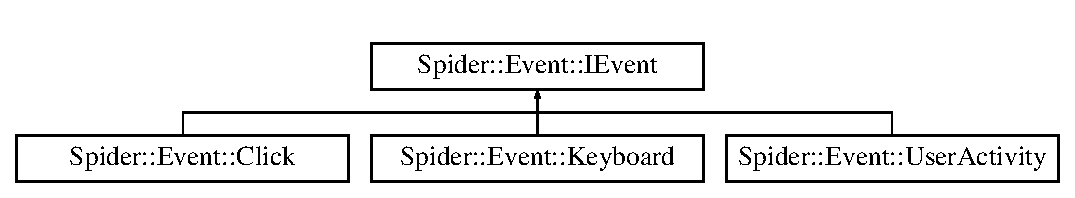
\includegraphics[height=2.000000cm]{class_spider_1_1_event_1_1_i_event}
\end{center}
\end{figure}
\subsection*{Public Member Functions}
\begin{DoxyCompactItemize}
\item 
\hyperlink{class_spider_1_1_event_1_1_i_event_aaebd414668b8f358b5cc1bc655038256}{I\+Event} (const std\+::string \&activity)
\begin{DoxyCompactList}\small\item\em Default constructor. \end{DoxyCompactList}\item 
\mbox{\Hypertarget{class_spider_1_1_event_1_1_i_event_a2e19a700707a4f951575dabf2af20cb1}\label{class_spider_1_1_event_1_1_i_event_a2e19a700707a4f951575dabf2af20cb1}} 
\hyperlink{class_spider_1_1_event_1_1_i_event_a2e19a700707a4f951575dabf2af20cb1}{I\+Event} (const \hyperlink{class_spider_1_1_event_1_1_i_event}{I\+Event} \&)=delete
\begin{DoxyCompactList}\small\item\em Default copy constructor. \end{DoxyCompactList}\item 
\hyperlink{class_spider_1_1_event_1_1_i_event}{I\+Event} \& \hyperlink{class_spider_1_1_event_1_1_i_event_a644158f21b7bf172d099819e23d1033e}{operator=} (const \hyperlink{class_spider_1_1_event_1_1_i_event}{I\+Event} \&)=delete
\begin{DoxyCompactList}\small\item\em Operator equal overlaod. \end{DoxyCompactList}\item 
\mbox{\Hypertarget{class_spider_1_1_event_1_1_i_event_a7494be717cfb8f0842b15446a14a655b}\label{class_spider_1_1_event_1_1_i_event_a7494be717cfb8f0842b15446a14a655b}} 
virtual \hyperlink{class_spider_1_1_event_1_1_i_event_a7494be717cfb8f0842b15446a14a655b}{$\sim$\+I\+Event} ()=default
\begin{DoxyCompactList}\small\item\em Default destroyer. \end{DoxyCompactList}\item 
virtual std\+::string \hyperlink{class_spider_1_1_event_1_1_i_event_ac8471df73080237faea55de539d968a0}{get\+Event\+Info} () const =0
\begin{DoxyCompactList}\small\item\em Extract \hyperlink{namespace_spider_1_1_event}{Event} information. \end{DoxyCompactList}\item 
virtual int \hyperlink{class_spider_1_1_event_1_1_i_event_a902d1376faa8e5948fa5bfe8d7208c88}{get\+Id} () const =0
\begin{DoxyCompactList}\small\item\em Get id of the event. \end{DoxyCompactList}\end{DoxyCompactItemize}
\subsection*{Protected Attributes}
\begin{DoxyCompactItemize}
\item 
\mbox{\Hypertarget{class_spider_1_1_event_1_1_i_event_a07aaa4ec795b2b70c10e34e832ec7b71}\label{class_spider_1_1_event_1_1_i_event_a07aaa4ec795b2b70c10e34e832ec7b71}} 
std\+::string \hyperlink{class_spider_1_1_event_1_1_i_event_a07aaa4ec795b2b70c10e34e832ec7b71}{m\+Process\+Info}
\begin{DoxyCompactList}\small\item\em actual process register \end{DoxyCompactList}\end{DoxyCompactItemize}


\subsection{Detailed Description}
\hyperlink{namespace_spider_1_1_event}{Event} interface. 

\subsection{Constructor \& Destructor Documentation}
\mbox{\Hypertarget{class_spider_1_1_event_1_1_i_event_aaebd414668b8f358b5cc1bc655038256}\label{class_spider_1_1_event_1_1_i_event_aaebd414668b8f358b5cc1bc655038256}} 
\index{Spider\+::\+Event\+::\+I\+Event@{Spider\+::\+Event\+::\+I\+Event}!I\+Event@{I\+Event}}
\index{I\+Event@{I\+Event}!Spider\+::\+Event\+::\+I\+Event@{Spider\+::\+Event\+::\+I\+Event}}
\subsubsection{\texorpdfstring{I\+Event()}{IEvent()}}
{\footnotesize\ttfamily Spider\+::\+Event\+::\+I\+Event\+::\+I\+Event (\begin{DoxyParamCaption}\item[{const std\+::string \&}]{activity }\end{DoxyParamCaption})\hspace{0.3cm}{\ttfamily [inline]}}



Default constructor. 


\begin{DoxyParams}{Parameters}
{\em last} & activity register \\
\hline
\end{DoxyParams}


\subsection{Member Function Documentation}
\mbox{\Hypertarget{class_spider_1_1_event_1_1_i_event_ac8471df73080237faea55de539d968a0}\label{class_spider_1_1_event_1_1_i_event_ac8471df73080237faea55de539d968a0}} 
\index{Spider\+::\+Event\+::\+I\+Event@{Spider\+::\+Event\+::\+I\+Event}!get\+Event\+Info@{get\+Event\+Info}}
\index{get\+Event\+Info@{get\+Event\+Info}!Spider\+::\+Event\+::\+I\+Event@{Spider\+::\+Event\+::\+I\+Event}}
\subsubsection{\texorpdfstring{get\+Event\+Info()}{getEventInfo()}}
{\footnotesize\ttfamily virtual std\+::string Spider\+::\+Event\+::\+I\+Event\+::get\+Event\+Info (\begin{DoxyParamCaption}{ }\end{DoxyParamCaption}) const\hspace{0.3cm}{\ttfamily [pure virtual]}}



Extract \hyperlink{namespace_spider_1_1_event}{Event} information. 

\begin{DoxyReturn}{Returns}
Informations into string format 
\end{DoxyReturn}


Implemented in \hyperlink{class_spider_1_1_event_1_1_keyboard_a3ea8239e9f2002ea2a4eb5dd0bbbb55a}{Spider\+::\+Event\+::\+Keyboard}, \hyperlink{class_spider_1_1_event_1_1_click_a916e746dc2145859f697de4d9f64cd00}{Spider\+::\+Event\+::\+Click}, and \hyperlink{class_spider_1_1_event_1_1_user_activity_a72d2436a1d9b339cc1cb1950f374562f}{Spider\+::\+Event\+::\+User\+Activity}.

\mbox{\Hypertarget{class_spider_1_1_event_1_1_i_event_a902d1376faa8e5948fa5bfe8d7208c88}\label{class_spider_1_1_event_1_1_i_event_a902d1376faa8e5948fa5bfe8d7208c88}} 
\index{Spider\+::\+Event\+::\+I\+Event@{Spider\+::\+Event\+::\+I\+Event}!get\+Id@{get\+Id}}
\index{get\+Id@{get\+Id}!Spider\+::\+Event\+::\+I\+Event@{Spider\+::\+Event\+::\+I\+Event}}
\subsubsection{\texorpdfstring{get\+Id()}{getId()}}
{\footnotesize\ttfamily virtual int Spider\+::\+Event\+::\+I\+Event\+::get\+Id (\begin{DoxyParamCaption}{ }\end{DoxyParamCaption}) const\hspace{0.3cm}{\ttfamily [pure virtual]}}



Get id of the event. 

\begin{DoxyReturn}{Returns}
\hyperlink{class_spider_1_1_event_1_1_request}{Request} ID 
\end{DoxyReturn}


Implemented in \hyperlink{class_spider_1_1_event_1_1_keyboard_aea1252251ac9ee1c7b71d0b0fcc7cc0a}{Spider\+::\+Event\+::\+Keyboard}, \hyperlink{class_spider_1_1_event_1_1_click_a32b810199a69b799589b680bfb9c287d}{Spider\+::\+Event\+::\+Click}, and \hyperlink{class_spider_1_1_event_1_1_user_activity_aabcbc7060a3f015b71f0b26b475ccf75}{Spider\+::\+Event\+::\+User\+Activity}.

\mbox{\Hypertarget{class_spider_1_1_event_1_1_i_event_a644158f21b7bf172d099819e23d1033e}\label{class_spider_1_1_event_1_1_i_event_a644158f21b7bf172d099819e23d1033e}} 
\index{Spider\+::\+Event\+::\+I\+Event@{Spider\+::\+Event\+::\+I\+Event}!operator=@{operator=}}
\index{operator=@{operator=}!Spider\+::\+Event\+::\+I\+Event@{Spider\+::\+Event\+::\+I\+Event}}
\subsubsection{\texorpdfstring{operator=()}{operator=()}}
{\footnotesize\ttfamily \hyperlink{class_spider_1_1_event_1_1_i_event}{I\+Event}\& Spider\+::\+Event\+::\+I\+Event\+::operator= (\begin{DoxyParamCaption}\item[{const \hyperlink{class_spider_1_1_event_1_1_i_event}{I\+Event} \&}]{ }\end{DoxyParamCaption})\hspace{0.3cm}{\ttfamily [delete]}}



Operator equal overlaod. 

\begin{DoxyReturn}{Returns}
\hyperlink{namespace_spider_1_1_event}{Event} interface 
\end{DoxyReturn}


The documentation for this class was generated from the following file\+:\begin{DoxyCompactItemize}
\item 
Event/\hyperlink{_i_event_8hpp}{I\+Event.\+hpp}\end{DoxyCompactItemize}

\hypertarget{class_spider_1_1_event_1_1_keyboard}{}\section{Spider\+:\+:Event\+:\+:Keyboard Class Reference}
\label{class_spider_1_1_event_1_1_keyboard}\index{Spider\+::\+Event\+::\+Keyboard@{Spider\+::\+Event\+::\+Keyboard}}


\hyperlink{class_spider_1_1_event_1_1_keyboard}{Keyboard} Handler.  




{\ttfamily \#include $<$Keyboard.\+hpp$>$}

Inheritance diagram for Spider\+:\+:Event\+:\+:Keyboard\+:\begin{figure}[H]
\begin{center}
\leavevmode
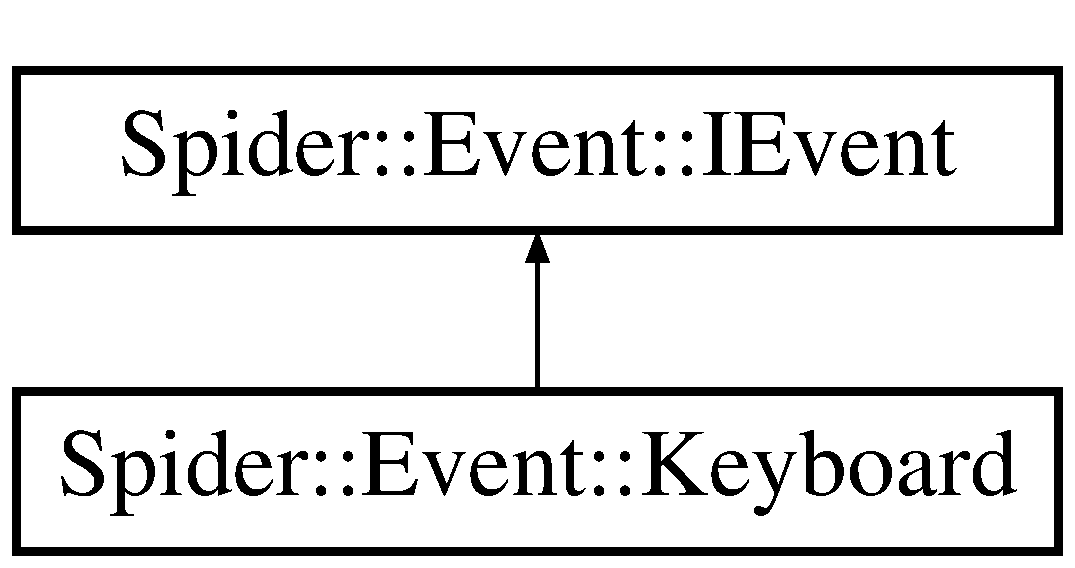
\includegraphics[height=2.000000cm]{class_spider_1_1_event_1_1_keyboard}
\end{center}
\end{figure}
\subsection*{Public Member Functions}
\begin{DoxyCompactItemize}
\item 
\hyperlink{class_spider_1_1_event_1_1_keyboard_a1fd20c190955bbe2856124e7f41dd8b7}{Keyboard} (const std\+::string \&activity)
\begin{DoxyCompactList}\small\item\em Default constructor. \end{DoxyCompactList}\item 
\mbox{\Hypertarget{class_spider_1_1_event_1_1_keyboard_abe0da2633d327af5b491b02333616d65}\label{class_spider_1_1_event_1_1_keyboard_abe0da2633d327af5b491b02333616d65}} 
\hyperlink{class_spider_1_1_event_1_1_keyboard_abe0da2633d327af5b491b02333616d65}{Keyboard} (const \hyperlink{class_spider_1_1_event_1_1_keyboard}{Keyboard} \&)=delete
\begin{DoxyCompactList}\small\item\em Default copy constructor. \end{DoxyCompactList}\item 
\hyperlink{class_spider_1_1_event_1_1_keyboard}{Keyboard} \& \hyperlink{class_spider_1_1_event_1_1_keyboard_a4b6e022f756523104222e71d1d59fd54}{operator=} (const \hyperlink{class_spider_1_1_event_1_1_keyboard}{Keyboard} \&)=delete
\begin{DoxyCompactList}\small\item\em Operator equal overlaod. \end{DoxyCompactList}\item 
\mbox{\Hypertarget{class_spider_1_1_event_1_1_keyboard_a2b7799295335ac4bea0bc4c3089b7b50}\label{class_spider_1_1_event_1_1_keyboard_a2b7799295335ac4bea0bc4c3089b7b50}} 
virtual \hyperlink{class_spider_1_1_event_1_1_keyboard_a2b7799295335ac4bea0bc4c3089b7b50}{$\sim$\+Keyboard} ()=default
\begin{DoxyCompactList}\small\item\em Default destroyer. \end{DoxyCompactList}\item 
virtual std\+::string \hyperlink{class_spider_1_1_event_1_1_keyboard_a3ea8239e9f2002ea2a4eb5dd0bbbb55a}{get\+Event\+Info} () const
\begin{DoxyCompactList}\small\item\em Extract \hyperlink{class_spider_1_1_event_1_1_keyboard}{Keyboard} information. \end{DoxyCompactList}\item 
virtual int \hyperlink{class_spider_1_1_event_1_1_keyboard_aea1252251ac9ee1c7b71d0b0fcc7cc0a}{get\+Id} () const
\begin{DoxyCompactList}\small\item\em Get id of the event. \end{DoxyCompactList}\item 
void \hyperlink{class_spider_1_1_event_1_1_keyboard_adde706a751b1df210bb459dcc33c05a8}{set\+Key} (int key)
\begin{DoxyCompactList}\small\item\em save key catch by the keylogger \end{DoxyCompactList}\item 
bool \hyperlink{class_spider_1_1_event_1_1_keyboard_a3d89487e20e8ad9f2d0889e0c57858e5}{is\+Special\+Char} (int key)
\begin{DoxyCompactList}\small\item\em check if the key catch is a special character \end{DoxyCompactList}\end{DoxyCompactItemize}
\subsection*{Additional Inherited Members}


\subsection{Detailed Description}
\hyperlink{class_spider_1_1_event_1_1_keyboard}{Keyboard} Handler. 

\subsection{Constructor \& Destructor Documentation}
\mbox{\Hypertarget{class_spider_1_1_event_1_1_keyboard_a1fd20c190955bbe2856124e7f41dd8b7}\label{class_spider_1_1_event_1_1_keyboard_a1fd20c190955bbe2856124e7f41dd8b7}} 
\index{Spider\+::\+Event\+::\+Keyboard@{Spider\+::\+Event\+::\+Keyboard}!Keyboard@{Keyboard}}
\index{Keyboard@{Keyboard}!Spider\+::\+Event\+::\+Keyboard@{Spider\+::\+Event\+::\+Keyboard}}
\subsubsection{\texorpdfstring{Keyboard()}{Keyboard()}}
{\footnotesize\ttfamily Spider\+::\+Event\+::\+Keyboard\+::\+Keyboard (\begin{DoxyParamCaption}\item[{const std\+::string \&}]{activity }\end{DoxyParamCaption})\hspace{0.3cm}{\ttfamily [inline]}}



Default constructor. 


\begin{DoxyParams}{Parameters}
{\em last} & activity register \\
\hline
\end{DoxyParams}


\subsection{Member Function Documentation}
\mbox{\Hypertarget{class_spider_1_1_event_1_1_keyboard_a3ea8239e9f2002ea2a4eb5dd0bbbb55a}\label{class_spider_1_1_event_1_1_keyboard_a3ea8239e9f2002ea2a4eb5dd0bbbb55a}} 
\index{Spider\+::\+Event\+::\+Keyboard@{Spider\+::\+Event\+::\+Keyboard}!get\+Event\+Info@{get\+Event\+Info}}
\index{get\+Event\+Info@{get\+Event\+Info}!Spider\+::\+Event\+::\+Keyboard@{Spider\+::\+Event\+::\+Keyboard}}
\subsubsection{\texorpdfstring{get\+Event\+Info()}{getEventInfo()}}
{\footnotesize\ttfamily virtual std\+::string Spider\+::\+Event\+::\+Keyboard\+::get\+Event\+Info (\begin{DoxyParamCaption}{ }\end{DoxyParamCaption}) const\hspace{0.3cm}{\ttfamily [virtual]}}



Extract \hyperlink{class_spider_1_1_event_1_1_keyboard}{Keyboard} information. 

\begin{DoxyReturn}{Returns}
Informations into string format 
\end{DoxyReturn}


Implements \hyperlink{class_spider_1_1_event_1_1_i_event_ac8471df73080237faea55de539d968a0}{Spider\+::\+Event\+::\+I\+Event}.

\mbox{\Hypertarget{class_spider_1_1_event_1_1_keyboard_aea1252251ac9ee1c7b71d0b0fcc7cc0a}\label{class_spider_1_1_event_1_1_keyboard_aea1252251ac9ee1c7b71d0b0fcc7cc0a}} 
\index{Spider\+::\+Event\+::\+Keyboard@{Spider\+::\+Event\+::\+Keyboard}!get\+Id@{get\+Id}}
\index{get\+Id@{get\+Id}!Spider\+::\+Event\+::\+Keyboard@{Spider\+::\+Event\+::\+Keyboard}}
\subsubsection{\texorpdfstring{get\+Id()}{getId()}}
{\footnotesize\ttfamily virtual int Spider\+::\+Event\+::\+Keyboard\+::get\+Id (\begin{DoxyParamCaption}{ }\end{DoxyParamCaption}) const\hspace{0.3cm}{\ttfamily [inline]}, {\ttfamily [virtual]}}



Get id of the event. 

\begin{DoxyReturn}{Returns}
\hyperlink{class_spider_1_1_event_1_1_request}{Request} ID 
\end{DoxyReturn}


Implements \hyperlink{class_spider_1_1_event_1_1_i_event_a902d1376faa8e5948fa5bfe8d7208c88}{Spider\+::\+Event\+::\+I\+Event}.

\mbox{\Hypertarget{class_spider_1_1_event_1_1_keyboard_a3d89487e20e8ad9f2d0889e0c57858e5}\label{class_spider_1_1_event_1_1_keyboard_a3d89487e20e8ad9f2d0889e0c57858e5}} 
\index{Spider\+::\+Event\+::\+Keyboard@{Spider\+::\+Event\+::\+Keyboard}!is\+Special\+Char@{is\+Special\+Char}}
\index{is\+Special\+Char@{is\+Special\+Char}!Spider\+::\+Event\+::\+Keyboard@{Spider\+::\+Event\+::\+Keyboard}}
\subsubsection{\texorpdfstring{is\+Special\+Char()}{isSpecialChar()}}
{\footnotesize\ttfamily bool Spider\+::\+Event\+::\+Keyboard\+::is\+Special\+Char (\begin{DoxyParamCaption}\item[{int}]{key }\end{DoxyParamCaption})}



check if the key catch is a special character 


\begin{DoxyParams}{Parameters}
{\em last} & key register \\
\hline
\end{DoxyParams}
\begin{DoxyReturn}{Returns}
true if it\textquotesingle{}s a special char, overwise false 
\end{DoxyReturn}
\mbox{\Hypertarget{class_spider_1_1_event_1_1_keyboard_a4b6e022f756523104222e71d1d59fd54}\label{class_spider_1_1_event_1_1_keyboard_a4b6e022f756523104222e71d1d59fd54}} 
\index{Spider\+::\+Event\+::\+Keyboard@{Spider\+::\+Event\+::\+Keyboard}!operator=@{operator=}}
\index{operator=@{operator=}!Spider\+::\+Event\+::\+Keyboard@{Spider\+::\+Event\+::\+Keyboard}}
\subsubsection{\texorpdfstring{operator=()}{operator=()}}
{\footnotesize\ttfamily \hyperlink{class_spider_1_1_event_1_1_keyboard}{Keyboard}\& Spider\+::\+Event\+::\+Keyboard\+::operator= (\begin{DoxyParamCaption}\item[{const \hyperlink{class_spider_1_1_event_1_1_keyboard}{Keyboard} \&}]{ }\end{DoxyParamCaption})\hspace{0.3cm}{\ttfamily [delete]}}



Operator equal overlaod. 

\begin{DoxyReturn}{Returns}
\hyperlink{class_spider_1_1_event_1_1_keyboard}{Keyboard} 
\end{DoxyReturn}
\mbox{\Hypertarget{class_spider_1_1_event_1_1_keyboard_adde706a751b1df210bb459dcc33c05a8}\label{class_spider_1_1_event_1_1_keyboard_adde706a751b1df210bb459dcc33c05a8}} 
\index{Spider\+::\+Event\+::\+Keyboard@{Spider\+::\+Event\+::\+Keyboard}!set\+Key@{set\+Key}}
\index{set\+Key@{set\+Key}!Spider\+::\+Event\+::\+Keyboard@{Spider\+::\+Event\+::\+Keyboard}}
\subsubsection{\texorpdfstring{set\+Key()}{setKey()}}
{\footnotesize\ttfamily void Spider\+::\+Event\+::\+Keyboard\+::set\+Key (\begin{DoxyParamCaption}\item[{int}]{key }\end{DoxyParamCaption})}



save key catch by the keylogger 


\begin{DoxyParams}{Parameters}
{\em last} & key register \\
\hline
\end{DoxyParams}


The documentation for this class was generated from the following file\+:\begin{DoxyCompactItemize}
\item 
Event/Keyboard.\+hpp\end{DoxyCompactItemize}

\hypertarget{class_spider_1_1_core_1_1_key_reader}{}\section{Spider\+:\+:Core\+:\+:Key\+Reader Class Reference}
\label{class_spider_1_1_core_1_1_key_reader}\index{Spider\+::\+Core\+::\+Key\+Reader@{Spider\+::\+Core\+::\+Key\+Reader}}


Read event.  




{\ttfamily \#include $<$Key\+Reader.\+hpp$>$}

\subsection*{Public Member Functions}
\begin{DoxyCompactItemize}
\item 
\mbox{\Hypertarget{class_spider_1_1_core_1_1_key_reader_a4d56368d7bd01a455130d6fb1f342463}\label{class_spider_1_1_core_1_1_key_reader_a4d56368d7bd01a455130d6fb1f342463}} 
\hyperlink{class_spider_1_1_core_1_1_key_reader_a4d56368d7bd01a455130d6fb1f342463}{Key\+Reader} ()
\begin{DoxyCompactList}\small\item\em Constructor. \end{DoxyCompactList}\item 
\mbox{\Hypertarget{class_spider_1_1_core_1_1_key_reader_ace2bf54fcbd10aea76f3afe0dc50c802}\label{class_spider_1_1_core_1_1_key_reader_ace2bf54fcbd10aea76f3afe0dc50c802}} 
\hyperlink{class_spider_1_1_core_1_1_key_reader_ace2bf54fcbd10aea76f3afe0dc50c802}{Key\+Reader} (const \hyperlink{class_spider_1_1_core_1_1_key_reader}{Key\+Reader} \&)=delete
\begin{DoxyCompactList}\small\item\em Default copy constructor. \end{DoxyCompactList}\item 
\hyperlink{class_spider_1_1_core_1_1_key_reader}{Key\+Reader} \& \hyperlink{class_spider_1_1_core_1_1_key_reader_a17eaa634915bdca4e3e32bac7a0bad39}{operator=} (const \hyperlink{class_spider_1_1_core_1_1_key_reader}{Key\+Reader} \&) const =delete
\begin{DoxyCompactList}\small\item\em Operator equal overlaod. \end{DoxyCompactList}\item 
\mbox{\Hypertarget{class_spider_1_1_core_1_1_key_reader_a7792d49fd03445cfdd3b72ad6a5009cb}\label{class_spider_1_1_core_1_1_key_reader_a7792d49fd03445cfdd3b72ad6a5009cb}} 
\hyperlink{class_spider_1_1_core_1_1_key_reader_a7792d49fd03445cfdd3b72ad6a5009cb}{$\sim$\+Key\+Reader} ()=default
\begin{DoxyCompactList}\small\item\em Default destroyer. \end{DoxyCompactList}\item 
void \hyperlink{class_spider_1_1_core_1_1_key_reader_a4b44cc097ccd3c508336217b4b17f8b4}{read} (\hyperlink{class_spider_1_1_event_1_1_event_queue}{Event\+::\+Event\+Queue} $\ast$queue)
\begin{DoxyCompactList}\small\item\em Read \hyperlink{namespace_spider_1_1_event}{Event} and push it in the queue. \end{DoxyCompactList}\end{DoxyCompactItemize}


\subsection{Detailed Description}
Read event. 

\subsection{Member Function Documentation}
\mbox{\Hypertarget{class_spider_1_1_core_1_1_key_reader_a17eaa634915bdca4e3e32bac7a0bad39}\label{class_spider_1_1_core_1_1_key_reader_a17eaa634915bdca4e3e32bac7a0bad39}} 
\index{Spider\+::\+Core\+::\+Key\+Reader@{Spider\+::\+Core\+::\+Key\+Reader}!operator=@{operator=}}
\index{operator=@{operator=}!Spider\+::\+Core\+::\+Key\+Reader@{Spider\+::\+Core\+::\+Key\+Reader}}
\subsubsection{\texorpdfstring{operator=()}{operator=()}}
{\footnotesize\ttfamily \hyperlink{class_spider_1_1_core_1_1_key_reader}{Key\+Reader}\& Spider\+::\+Core\+::\+Key\+Reader\+::operator= (\begin{DoxyParamCaption}\item[{const \hyperlink{class_spider_1_1_core_1_1_key_reader}{Key\+Reader} \&}]{ }\end{DoxyParamCaption}) const\hspace{0.3cm}{\ttfamily [delete]}}



Operator equal overlaod. 

\begin{DoxyReturn}{Returns}
\hyperlink{class_spider_1_1_core_1_1_key_reader}{Key\+Reader} 
\end{DoxyReturn}
\mbox{\Hypertarget{class_spider_1_1_core_1_1_key_reader_a4b44cc097ccd3c508336217b4b17f8b4}\label{class_spider_1_1_core_1_1_key_reader_a4b44cc097ccd3c508336217b4b17f8b4}} 
\index{Spider\+::\+Core\+::\+Key\+Reader@{Spider\+::\+Core\+::\+Key\+Reader}!read@{read}}
\index{read@{read}!Spider\+::\+Core\+::\+Key\+Reader@{Spider\+::\+Core\+::\+Key\+Reader}}
\subsubsection{\texorpdfstring{read()}{read()}}
{\footnotesize\ttfamily void Spider\+::\+Core\+::\+Key\+Reader\+::read (\begin{DoxyParamCaption}\item[{\hyperlink{class_spider_1_1_event_1_1_event_queue}{Event\+::\+Event\+Queue} $\ast$}]{queue }\end{DoxyParamCaption})}



Read \hyperlink{namespace_spider_1_1_event}{Event} and push it in the queue. 


\begin{DoxyParams}{Parameters}
{\em queue} & of I\+Event \\
\hline
\end{DoxyParams}


The documentation for this class was generated from the following file\+:\begin{DoxyCompactItemize}
\item 
Core/\hyperlink{_key_reader_8hpp}{Key\+Reader.\+hpp}\end{DoxyCompactItemize}

\hypertarget{structts_1_1common_1_1_packet}{}\section{ts\+:\+:common\+:\+:Packet Struct Reference}
\label{structts_1_1common_1_1_packet}\index{ts\+::common\+::\+Packet@{ts\+::common\+::\+Packet}}
\subsection*{Public Attributes}
\begin{DoxyCompactItemize}
\item 
\mbox{\Hypertarget{structts_1_1common_1_1_packet_a22cf5cbe00488c2f324bc580b43b332b}\label{structts_1_1common_1_1_packet_a22cf5cbe00488c2f324bc580b43b332b}} 
\hyperlink{structts_1_1common_1_1_packet_header}{Packet\+Header} {\bfseries header} \{\}
\item 
\mbox{\Hypertarget{structts_1_1common_1_1_packet_ae1df6eb6a4d7307e68369a144a0c6a51}\label{structts_1_1common_1_1_packet_ae1df6eb6a4d7307e68369a144a0c6a51}} 
\hyperlink{structts_1_1common_1_1_packet_body}{Packet\+Body} {\bfseries body} \{\}
\end{DoxyCompactItemize}


The documentation for this struct was generated from the following file\+:\begin{DoxyCompactItemize}
\item 
Socket/Packet.\+hpp\end{DoxyCompactItemize}

\hypertarget{structts_1_1common_1_1_packet_body}{}\section{ts\+:\+:common\+:\+:Packet\+Body Struct Reference}
\label{structts_1_1common_1_1_packet_body}\index{ts\+::common\+::\+Packet\+Body@{ts\+::common\+::\+Packet\+Body}}
\subsection*{Public Member Functions}
\begin{DoxyCompactItemize}
\item 
\mbox{\Hypertarget{structts_1_1common_1_1_packet_body_a2a7de4788181d825b0187aabe71354ec}\label{structts_1_1common_1_1_packet_body_a2a7de4788181d825b0187aabe71354ec}} 
void \hyperlink{structts_1_1common_1_1_packet_body_a2a7de4788181d825b0187aabe71354ec}{reset} ()
\begin{DoxyCompactList}\small\item\em Reset data in body. \end{DoxyCompactList}\end{DoxyCompactItemize}
\subsection*{Public Attributes}
\begin{DoxyCompactItemize}
\item 
\mbox{\Hypertarget{structts_1_1common_1_1_packet_body_ac209e31fb1a4d1024061a4949d923ff0}\label{structts_1_1common_1_1_packet_body_ac209e31fb1a4d1024061a4949d923ff0}} 
char $\ast$ {\bfseries data}
\end{DoxyCompactItemize}


The documentation for this struct was generated from the following file\+:\begin{DoxyCompactItemize}
\item 
Packet/Packet.\+hpp\end{DoxyCompactItemize}

\hypertarget{structts_1_1common_1_1_packet_header}{}\section{ts\+:\+:common\+:\+:Packet\+Header Struct Reference}
\label{structts_1_1common_1_1_packet_header}\index{ts\+::common\+::\+Packet\+Header@{ts\+::common\+::\+Packet\+Header}}
\subsection*{Public Member Functions}
\begin{DoxyCompactItemize}
\item 
\mbox{\Hypertarget{structts_1_1common_1_1_packet_header_adf4e5e691171eeac8d38f8d0ddf3e138}\label{structts_1_1common_1_1_packet_header_adf4e5e691171eeac8d38f8d0ddf3e138}} 
void \hyperlink{structts_1_1common_1_1_packet_header_adf4e5e691171eeac8d38f8d0ddf3e138}{reset} ()
\begin{DoxyCompactList}\small\item\em Reset data in header. \end{DoxyCompactList}\end{DoxyCompactItemize}
\subsection*{Public Attributes}
\begin{DoxyCompactItemize}
\item 
\mbox{\Hypertarget{structts_1_1common_1_1_packet_header_a95214ffcb1c52edd7a6282c2e6a40025}\label{structts_1_1common_1_1_packet_header_a95214ffcb1c52edd7a6282c2e6a40025}} 
int {\bfseries id}
\item 
\mbox{\Hypertarget{structts_1_1common_1_1_packet_header_a5dc7af4be3fbff0ca3756202450fe882}\label{structts_1_1common_1_1_packet_header_a5dc7af4be3fbff0ca3756202450fe882}} 
int {\bfseries size}
\end{DoxyCompactItemize}


The documentation for this struct was generated from the following file\+:\begin{DoxyCompactItemize}
\item 
Packet/Packet.\+hpp\end{DoxyCompactItemize}

\hypertarget{classts_1_1common_1_1_packet_manager}{}\section{ts\+:\+:common\+:\+:Packet\+Manager Class Reference}
\label{classts_1_1common_1_1_packet_manager}\index{ts\+::common\+::\+Packet\+Manager@{ts\+::common\+::\+Packet\+Manager}}
\subsection*{Public Member Functions}
\begin{DoxyCompactItemize}
\item 
\mbox{\Hypertarget{classts_1_1common_1_1_packet_manager_a3b73116e602124697590afecb82ef9fd}\label{classts_1_1common_1_1_packet_manager_a3b73116e602124697590afecb82ef9fd}} 
{\bfseries Packet\+Manager} (\hyperlink{classts_1_1common_1_1tcp_1_1_client_socket}{common\+::tcp\+::\+Client\+Socket} \&client\+Socket)
\item 
\mbox{\Hypertarget{classts_1_1common_1_1_packet_manager_a6165799da03af1c119d921ac96a24562}\label{classts_1_1common_1_1_packet_manager_a6165799da03af1c119d921ac96a24562}} 
void {\bfseries async\+Read} (On\+Read\+Complete\+Packet on\+Read\+Complete\+Packet, On\+Read\+Packet\+Error on\+Read\+Packet\+Error)
\item 
\mbox{\Hypertarget{classts_1_1common_1_1_packet_manager_ae308b816f8cf10367f0f63fa5c1fadf4}\label{classts_1_1common_1_1_packet_manager_ae308b816f8cf10367f0f63fa5c1fadf4}} 
void {\bfseries async\+Write} (std\+::shared\+\_\+ptr$<$ \hyperlink{structts_1_1common_1_1_packet}{Packet} $>$ const \&packet, On\+Write\+Complete\+Packet on\+Write\+Complete\+Packet, On\+Write\+Packet\+Error on\+Write\+Packet\+Error)
\item 
\mbox{\Hypertarget{classts_1_1common_1_1_packet_manager_aae446c8e99adc8ead7d4b0cd40545cd0}\label{classts_1_1common_1_1_packet_manager_aae446c8e99adc8ead7d4b0cd40545cd0}} 
void {\bfseries send} (int packet\+Header\+Id, std\+::string const \&data, On\+Write\+Complete\+Packet on\+Write\+Complete\+Packet, On\+Write\+Packet\+Error on\+Write\+Packet\+Error)
\end{DoxyCompactItemize}


The documentation for this class was generated from the following file\+:\begin{DoxyCompactItemize}
\item 
Socket/Packet\+Manager.\+hpp\end{DoxyCompactItemize}

\hypertarget{class_spider_1_1_event_1_1_request}{}\section{Spider\+:\+:Event\+:\+:Request Class Reference}
\label{class_spider_1_1_event_1_1_request}\index{Spider\+::\+Event\+::\+Request@{Spider\+::\+Event\+::\+Request}}


\hyperlink{class_spider_1_1_event_1_1_request}{Request} informations container.  




{\ttfamily \#include $<$Request.\+hpp$>$}

\subsection*{Public Member Functions}
\begin{DoxyCompactItemize}
\item 
\mbox{\Hypertarget{class_spider_1_1_event_1_1_request_ad141d09686cf9cdb1ecb9eba82b2710b}\label{class_spider_1_1_event_1_1_request_ad141d09686cf9cdb1ecb9eba82b2710b}} 
\hyperlink{class_spider_1_1_event_1_1_request_ad141d09686cf9cdb1ecb9eba82b2710b}{Request} ()
\begin{DoxyCompactList}\small\item\em Default constructor. \end{DoxyCompactList}\item 
\mbox{\Hypertarget{class_spider_1_1_event_1_1_request_a65c49a1885b979b125adcbad72ab73ee}\label{class_spider_1_1_event_1_1_request_a65c49a1885b979b125adcbad72ab73ee}} 
\hyperlink{class_spider_1_1_event_1_1_request_a65c49a1885b979b125adcbad72ab73ee}{Request} (const \hyperlink{class_spider_1_1_event_1_1_request}{Request} \&request)
\begin{DoxyCompactList}\small\item\em Default copy constructor. \end{DoxyCompactList}\item 
\mbox{\Hypertarget{class_spider_1_1_event_1_1_request_aa6c13b33959dc082e00b9c872d41c84d}\label{class_spider_1_1_event_1_1_request_aa6c13b33959dc082e00b9c872d41c84d}} 
\hyperlink{class_spider_1_1_event_1_1_request}{Request} \& \hyperlink{class_spider_1_1_event_1_1_request_aa6c13b33959dc082e00b9c872d41c84d}{operator=} (const \hyperlink{class_spider_1_1_event_1_1_request}{Request} \&request)=delete
\begin{DoxyCompactList}\small\item\em Equal operator overload. \end{DoxyCompactList}\item 
\mbox{\Hypertarget{class_spider_1_1_event_1_1_request_a7da7773ecc691187761673918cd7def2}\label{class_spider_1_1_event_1_1_request_a7da7773ecc691187761673918cd7def2}} 
\hyperlink{class_spider_1_1_event_1_1_request_a7da7773ecc691187761673918cd7def2}{$\sim$\+Request} ()=default
\begin{DoxyCompactList}\small\item\em Default destructor. \end{DoxyCompactList}\item 
std\+::string \hyperlink{class_spider_1_1_event_1_1_request_adf63bc8d31f15530f110227b8827aabd}{generate} (int request\+Id, const \hyperlink{class_spider_1_1ssl_1_1_r_s_a_keys}{ssl\+::\+R\+S\+A\+Keys} \&rsa, bool is\+Crypt) const
\begin{DoxyCompactList}\small\item\em \hyperlink{class_spider_1_1_event_1_1_request}{Request} generator. \end{DoxyCompactList}\end{DoxyCompactItemize}
\subsection*{Public Attributes}
\begin{DoxyCompactItemize}
\item 
\mbox{\Hypertarget{class_spider_1_1_event_1_1_request_a9fa54e719d09318f76a13abe503feba0}\label{class_spider_1_1_event_1_1_request_a9fa54e719d09318f76a13abe503feba0}} 
size\+\_\+t \hyperlink{class_spider_1_1_event_1_1_request_a9fa54e719d09318f76a13abe503feba0}{m\+Request\+Idx}
\begin{DoxyCompactList}\small\item\em Idx from the request. \end{DoxyCompactList}\item 
\mbox{\Hypertarget{class_spider_1_1_event_1_1_request_aaa5e49fc54e2a9523b18788301ce43dc}\label{class_spider_1_1_event_1_1_request_aaa5e49fc54e2a9523b18788301ce43dc}} 
std\+::string \hyperlink{class_spider_1_1_event_1_1_request_aaa5e49fc54e2a9523b18788301ce43dc}{m\+From}
\begin{DoxyCompactList}\small\item\em Sender name. \end{DoxyCompactList}\item 
\mbox{\Hypertarget{class_spider_1_1_event_1_1_request_a4077565fee9e0610f706c3e28adfc314}\label{class_spider_1_1_event_1_1_request_a4077565fee9e0610f706c3e28adfc314}} 
std\+::string \hyperlink{class_spider_1_1_event_1_1_request_a4077565fee9e0610f706c3e28adfc314}{m\+To}
\begin{DoxyCompactList}\small\item\em Receiver name. \end{DoxyCompactList}\item 
\mbox{\Hypertarget{class_spider_1_1_event_1_1_request_a049065d188d2ece9a873b770c312355c}\label{class_spider_1_1_event_1_1_request_a049065d188d2ece9a873b770c312355c}} 
std\+::time\+\_\+t \hyperlink{class_spider_1_1_event_1_1_request_a049065d188d2ece9a873b770c312355c}{m\+Timestamp}
\begin{DoxyCompactList}\small\item\em Time where the package is create. \end{DoxyCompactList}\item 
\mbox{\Hypertarget{class_spider_1_1_event_1_1_request_a2d763ea57d53fe6b9cfd6b747fcc920e}\label{class_spider_1_1_event_1_1_request_a2d763ea57d53fe6b9cfd6b747fcc920e}} 
std\+::shared\+\_\+ptr$<$ \hyperlink{class_spider_1_1_event_1_1_i_event}{Event\+::\+I\+Event} $>$ \hyperlink{class_spider_1_1_event_1_1_request_a2d763ea57d53fe6b9cfd6b747fcc920e}{m\+Event}
\begin{DoxyCompactList}\small\item\em \hyperlink{namespace_spider_1_1_event}{Event} of request. \end{DoxyCompactList}\end{DoxyCompactItemize}


\subsection{Detailed Description}
\hyperlink{class_spider_1_1_event_1_1_request}{Request} informations container. 

\subsection{Member Function Documentation}
\mbox{\Hypertarget{class_spider_1_1_event_1_1_request_adf63bc8d31f15530f110227b8827aabd}\label{class_spider_1_1_event_1_1_request_adf63bc8d31f15530f110227b8827aabd}} 
\index{Spider\+::\+Event\+::\+Request@{Spider\+::\+Event\+::\+Request}!generate@{generate}}
\index{generate@{generate}!Spider\+::\+Event\+::\+Request@{Spider\+::\+Event\+::\+Request}}
\subsubsection{\texorpdfstring{generate()}{generate()}}
{\footnotesize\ttfamily std\+::string Spider\+::\+Event\+::\+Request\+::generate (\begin{DoxyParamCaption}\item[{int}]{request\+Id,  }\item[{const \hyperlink{class_spider_1_1ssl_1_1_r_s_a_keys}{ssl\+::\+R\+S\+A\+Keys} \&}]{rsa,  }\item[{bool}]{is\+Crypt }\end{DoxyParamCaption}) const}



\hyperlink{class_spider_1_1_event_1_1_request}{Request} generator. 


\begin{DoxyParams}{Parameters}
{\em request\+Id} & Id of the request to generate \\
\hline
{\em rsa} & R\+SA keys to crypt the data \\
\hline
{\em is\+Crypt} & Indicator to know if the request need to be crypted \\
\hline
\end{DoxyParams}


The documentation for this class was generated from the following file\+:\begin{DoxyCompactItemize}
\item 
Event/Request.\+hpp\end{DoxyCompactItemize}

\hypertarget{class_spider_1_1ssl_1_1_r_s_a_keys}{}\section{Spider\+:\+:ssl\+:\+:R\+S\+A\+Keys Class Reference}
\label{class_spider_1_1ssl_1_1_r_s_a_keys}\index{Spider\+::ssl\+::\+R\+S\+A\+Keys@{Spider\+::ssl\+::\+R\+S\+A\+Keys}}


Encapsulation of the open\+S\+SL one-\/way encryption system.  




{\ttfamily \#include $<$R\+S\+A\+Keys.\+hpp$>$}

\subsection*{Public Member Functions}
\begin{DoxyCompactItemize}
\item 
\hyperlink{class_spider_1_1ssl_1_1_r_s_a_keys_a656fbf95f4ea432cbdbe40c4f0cb57f2}{R\+S\+A\+Keys} ()
\begin{DoxyCompactList}\small\item\em R\+SA envelop keys. \end{DoxyCompactList}\item 
\mbox{\Hypertarget{class_spider_1_1ssl_1_1_r_s_a_keys_a7a6fada6e8459ac0bcc20766f9083bd5}\label{class_spider_1_1ssl_1_1_r_s_a_keys_a7a6fada6e8459ac0bcc20766f9083bd5}} 
\hyperlink{class_spider_1_1ssl_1_1_r_s_a_keys_a7a6fada6e8459ac0bcc20766f9083bd5}{R\+S\+A\+Keys} (const \hyperlink{class_spider_1_1ssl_1_1_r_s_a_keys}{R\+S\+A\+Keys} \&)=delete
\begin{DoxyCompactList}\small\item\em Copy constructor. \end{DoxyCompactList}\item 
\hyperlink{class_spider_1_1ssl_1_1_r_s_a_keys_a6dbecb26eadd6691d93a5f8d74ddce70}{R\+S\+A\+Keys} (const std\+::string \&path\+Private\+Key, const std\+::string path\+Public\+Key)
\begin{DoxyCompactList}\small\item\em Create R\+SA keys with the two keys path. \end{DoxyCompactList}\item 
\hyperlink{class_spider_1_1ssl_1_1_r_s_a_keys}{R\+S\+A\+Keys} \& \hyperlink{class_spider_1_1ssl_1_1_r_s_a_keys_aa51f09af42c08d805e34bf351f478adc}{operator=} (const \hyperlink{class_spider_1_1ssl_1_1_r_s_a_keys}{R\+S\+A\+Keys} \&)=delete
\begin{DoxyCompactList}\small\item\em Equal operator overload. \end{DoxyCompactList}\item 
\mbox{\Hypertarget{class_spider_1_1ssl_1_1_r_s_a_keys_ac602db5926f1318399bdc94b436c6c21}\label{class_spider_1_1ssl_1_1_r_s_a_keys_ac602db5926f1318399bdc94b436c6c21}} 
\hyperlink{class_spider_1_1ssl_1_1_r_s_a_keys_ac602db5926f1318399bdc94b436c6c21}{$\sim$\+R\+S\+A\+Keys} ()
\begin{DoxyCompactList}\small\item\em Default Destroyer. \end{DoxyCompactList}\item 
\mbox{\Hypertarget{class_spider_1_1ssl_1_1_r_s_a_keys_acd779c58e9168d10fef5468015af063e}\label{class_spider_1_1ssl_1_1_r_s_a_keys_acd779c58e9168d10fef5468015af063e}} 
void \hyperlink{class_spider_1_1ssl_1_1_r_s_a_keys_acd779c58e9168d10fef5468015af063e}{generate} ()
\begin{DoxyCompactList}\small\item\em Generate two keys (private and public) \end{DoxyCompactList}\item 
R\+SA $\ast$ \hyperlink{class_spider_1_1ssl_1_1_r_s_a_keys_afec6c4762821ae4179adebbef1e4ee66}{get\+Private} () const
\begin{DoxyCompactList}\small\item\em Extract the private key from the \hyperlink{class_spider_1_1ssl_1_1_r_s_a_keys}{R\+S\+A\+Keys} envelop. \end{DoxyCompactList}\item 
R\+SA $\ast$ \hyperlink{class_spider_1_1ssl_1_1_r_s_a_keys_afa3b28ea88c61b6ddf602e70843d6471}{get\+Public} () const
\begin{DoxyCompactList}\small\item\em Extract the public key from the \hyperlink{class_spider_1_1ssl_1_1_r_s_a_keys}{R\+S\+A\+Keys} envelop. \end{DoxyCompactList}\item 
bool \hyperlink{class_spider_1_1ssl_1_1_r_s_a_keys_ae9702fe70c7ec6ef761995dd0fbb6abf}{read\+Public\+Key} (const std\+::string \&path)
\begin{DoxyCompactList}\small\item\em Read and extract a public key from a file. \end{DoxyCompactList}\item 
bool \hyperlink{class_spider_1_1ssl_1_1_r_s_a_keys_a9d177902b9051cd1b064b6597f3a3697}{read\+Private\+Key} (const std\+::string \&path)
\begin{DoxyCompactList}\small\item\em Read and extract a private key from a file. \end{DoxyCompactList}\item 
void \hyperlink{class_spider_1_1ssl_1_1_r_s_a_keys_a765563842f5a69b424d72cab3a77b678}{write} (F\+I\+LE $\ast$public\+Key, F\+I\+LE $\ast$private\+Key)
\begin{DoxyCompactList}\small\item\em Print on stdout the public and private key. \end{DoxyCompactList}\item 
void \hyperlink{class_spider_1_1ssl_1_1_r_s_a_keys_aabe857dba27e4cc8bd1d2a09b65082b8}{R\+S\+A\+Keys\+::convert\+Private} (std\+::string \&pub\+Key, std\+::string \&priv\+Key)
\begin{DoxyCompactList}\small\item\em Convert the Private and public key into strings. \end{DoxyCompactList}\item 
unsigned char $\ast$ \hyperlink{class_spider_1_1ssl_1_1_r_s_a_keys_a9e391f7d87fe9a8f58119629ed80f9bb}{encrypt\+Public} (unsigned char $\ast$data, const size\+\_\+t \&clear\+Lenght, int \&crypted\+Lenght) const
\begin{DoxyCompactList}\small\item\em Encrypt data from a public key. \end{DoxyCompactList}\item 
unsigned char $\ast$ \hyperlink{class_spider_1_1ssl_1_1_r_s_a_keys_a69c6bda29d2dbec830038b1d0ae92ab0}{encrypt\+Private} (unsigned char $\ast$data, const size\+\_\+t \&clear\+Lenght, int \&crypted\+Lenght) const
\begin{DoxyCompactList}\small\item\em Encrypt data from a private key. \end{DoxyCompactList}\item 
unsigned char $\ast$ \hyperlink{class_spider_1_1ssl_1_1_r_s_a_keys_a9d981778deeb914140ea27e6144721b9}{decrypt\+Public} (unsigned char $\ast$data, size\+\_\+t lenght) const
\begin{DoxyCompactList}\small\item\em Decrypt data from a public key. \end{DoxyCompactList}\item 
unsigned char $\ast$ \hyperlink{class_spider_1_1ssl_1_1_r_s_a_keys_a732ddcc62a20324b3ba10a765276220d}{decrypt\+Private} (unsigned char $\ast$data, size\+\_\+t lenght) const
\begin{DoxyCompactList}\small\item\em Decrypt data from a private key. \end{DoxyCompactList}\end{DoxyCompactItemize}


\subsection{Detailed Description}
Encapsulation of the open\+S\+SL one-\/way encryption system. 

\subsection{Constructor \& Destructor Documentation}
\mbox{\Hypertarget{class_spider_1_1ssl_1_1_r_s_a_keys_a656fbf95f4ea432cbdbe40c4f0cb57f2}\label{class_spider_1_1ssl_1_1_r_s_a_keys_a656fbf95f4ea432cbdbe40c4f0cb57f2}} 
\index{Spider\+::ssl\+::\+R\+S\+A\+Keys@{Spider\+::ssl\+::\+R\+S\+A\+Keys}!R\+S\+A\+Keys@{R\+S\+A\+Keys}}
\index{R\+S\+A\+Keys@{R\+S\+A\+Keys}!Spider\+::ssl\+::\+R\+S\+A\+Keys@{Spider\+::ssl\+::\+R\+S\+A\+Keys}}
\subsubsection{\texorpdfstring{R\+S\+A\+Keys()}{RSAKeys()}\hspace{0.1cm}{\footnotesize\ttfamily [1/2]}}
{\footnotesize\ttfamily Spider\+::ssl\+::\+R\+S\+A\+Keys\+::\+R\+S\+A\+Keys (\begin{DoxyParamCaption}{ }\end{DoxyParamCaption})\hspace{0.3cm}{\ttfamily [inline]}}



R\+SA envelop keys. 

Default constructor \mbox{\Hypertarget{class_spider_1_1ssl_1_1_r_s_a_keys_a6dbecb26eadd6691d93a5f8d74ddce70}\label{class_spider_1_1ssl_1_1_r_s_a_keys_a6dbecb26eadd6691d93a5f8d74ddce70}} 
\index{Spider\+::ssl\+::\+R\+S\+A\+Keys@{Spider\+::ssl\+::\+R\+S\+A\+Keys}!R\+S\+A\+Keys@{R\+S\+A\+Keys}}
\index{R\+S\+A\+Keys@{R\+S\+A\+Keys}!Spider\+::ssl\+::\+R\+S\+A\+Keys@{Spider\+::ssl\+::\+R\+S\+A\+Keys}}
\subsubsection{\texorpdfstring{R\+S\+A\+Keys()}{RSAKeys()}\hspace{0.1cm}{\footnotesize\ttfamily [2/2]}}
{\footnotesize\ttfamily Spider\+::ssl\+::\+R\+S\+A\+Keys\+::\+R\+S\+A\+Keys (\begin{DoxyParamCaption}\item[{const std\+::string \&}]{path\+Private\+Key,  }\item[{const std\+::string}]{path\+Public\+Key }\end{DoxyParamCaption})}



Create R\+SA keys with the two keys path. 


\begin{DoxyParams}{Parameters}
{\em path\+Private\+Key} & Path to the private key \\
\hline
{\em path\+Public\+Key} & Path to the public key \\
\hline
\end{DoxyParams}


\subsection{Member Function Documentation}
\mbox{\Hypertarget{class_spider_1_1ssl_1_1_r_s_a_keys_a732ddcc62a20324b3ba10a765276220d}\label{class_spider_1_1ssl_1_1_r_s_a_keys_a732ddcc62a20324b3ba10a765276220d}} 
\index{Spider\+::ssl\+::\+R\+S\+A\+Keys@{Spider\+::ssl\+::\+R\+S\+A\+Keys}!decrypt\+Private@{decrypt\+Private}}
\index{decrypt\+Private@{decrypt\+Private}!Spider\+::ssl\+::\+R\+S\+A\+Keys@{Spider\+::ssl\+::\+R\+S\+A\+Keys}}
\subsubsection{\texorpdfstring{decrypt\+Private()}{decryptPrivate()}}
{\footnotesize\ttfamily unsigned char$\ast$ Spider\+::ssl\+::\+R\+S\+A\+Keys\+::decrypt\+Private (\begin{DoxyParamCaption}\item[{unsigned char $\ast$}]{data,  }\item[{size\+\_\+t}]{lenght }\end{DoxyParamCaption}) const}



Decrypt data from a private key. 


\begin{DoxyParams}{Parameters}
{\em data} & Data to decrypt \\
\hline
{\em lenght} & Lenght of the data \\
\hline
\end{DoxyParams}
\begin{DoxyReturn}{Returns}
Decrypted data 
\end{DoxyReturn}
\mbox{\Hypertarget{class_spider_1_1ssl_1_1_r_s_a_keys_a9d981778deeb914140ea27e6144721b9}\label{class_spider_1_1ssl_1_1_r_s_a_keys_a9d981778deeb914140ea27e6144721b9}} 
\index{Spider\+::ssl\+::\+R\+S\+A\+Keys@{Spider\+::ssl\+::\+R\+S\+A\+Keys}!decrypt\+Public@{decrypt\+Public}}
\index{decrypt\+Public@{decrypt\+Public}!Spider\+::ssl\+::\+R\+S\+A\+Keys@{Spider\+::ssl\+::\+R\+S\+A\+Keys}}
\subsubsection{\texorpdfstring{decrypt\+Public()}{decryptPublic()}}
{\footnotesize\ttfamily unsigned char$\ast$ Spider\+::ssl\+::\+R\+S\+A\+Keys\+::decrypt\+Public (\begin{DoxyParamCaption}\item[{unsigned char $\ast$}]{data,  }\item[{size\+\_\+t}]{lenght }\end{DoxyParamCaption}) const}



Decrypt data from a public key. 


\begin{DoxyParams}{Parameters}
{\em data} & Data to decrypt \\
\hline
{\em lenght} & Lenght of the data \\
\hline
\end{DoxyParams}
\begin{DoxyReturn}{Returns}
Decrypted data 
\end{DoxyReturn}
\mbox{\Hypertarget{class_spider_1_1ssl_1_1_r_s_a_keys_a69c6bda29d2dbec830038b1d0ae92ab0}\label{class_spider_1_1ssl_1_1_r_s_a_keys_a69c6bda29d2dbec830038b1d0ae92ab0}} 
\index{Spider\+::ssl\+::\+R\+S\+A\+Keys@{Spider\+::ssl\+::\+R\+S\+A\+Keys}!encrypt\+Private@{encrypt\+Private}}
\index{encrypt\+Private@{encrypt\+Private}!Spider\+::ssl\+::\+R\+S\+A\+Keys@{Spider\+::ssl\+::\+R\+S\+A\+Keys}}
\subsubsection{\texorpdfstring{encrypt\+Private()}{encryptPrivate()}}
{\footnotesize\ttfamily unsigned char$\ast$ Spider\+::ssl\+::\+R\+S\+A\+Keys\+::encrypt\+Private (\begin{DoxyParamCaption}\item[{unsigned char $\ast$}]{data,  }\item[{const size\+\_\+t \&}]{clear\+Lenght,  }\item[{int \&}]{crypted\+Lenght }\end{DoxyParamCaption}) const}



Encrypt data from a private key. 


\begin{DoxyParams}{Parameters}
{\em data} & Data to encrypt \\
\hline
{\em lenght} & Lenght of the data \\
\hline
\end{DoxyParams}
\begin{DoxyReturn}{Returns}
Encrypted data 
\end{DoxyReturn}
\mbox{\Hypertarget{class_spider_1_1ssl_1_1_r_s_a_keys_a9e391f7d87fe9a8f58119629ed80f9bb}\label{class_spider_1_1ssl_1_1_r_s_a_keys_a9e391f7d87fe9a8f58119629ed80f9bb}} 
\index{Spider\+::ssl\+::\+R\+S\+A\+Keys@{Spider\+::ssl\+::\+R\+S\+A\+Keys}!encrypt\+Public@{encrypt\+Public}}
\index{encrypt\+Public@{encrypt\+Public}!Spider\+::ssl\+::\+R\+S\+A\+Keys@{Spider\+::ssl\+::\+R\+S\+A\+Keys}}
\subsubsection{\texorpdfstring{encrypt\+Public()}{encryptPublic()}}
{\footnotesize\ttfamily unsigned char$\ast$ Spider\+::ssl\+::\+R\+S\+A\+Keys\+::encrypt\+Public (\begin{DoxyParamCaption}\item[{unsigned char $\ast$}]{data,  }\item[{const size\+\_\+t \&}]{clear\+Lenght,  }\item[{int \&}]{crypted\+Lenght }\end{DoxyParamCaption}) const}



Encrypt data from a public key. 


\begin{DoxyParams}{Parameters}
{\em data} & Data to encrypt \\
\hline
{\em lenght} & Lenght of the data \\
\hline
\end{DoxyParams}
\begin{DoxyReturn}{Returns}
Encrypted data 
\end{DoxyReturn}
\mbox{\Hypertarget{class_spider_1_1ssl_1_1_r_s_a_keys_afec6c4762821ae4179adebbef1e4ee66}\label{class_spider_1_1ssl_1_1_r_s_a_keys_afec6c4762821ae4179adebbef1e4ee66}} 
\index{Spider\+::ssl\+::\+R\+S\+A\+Keys@{Spider\+::ssl\+::\+R\+S\+A\+Keys}!get\+Private@{get\+Private}}
\index{get\+Private@{get\+Private}!Spider\+::ssl\+::\+R\+S\+A\+Keys@{Spider\+::ssl\+::\+R\+S\+A\+Keys}}
\subsubsection{\texorpdfstring{get\+Private()}{getPrivate()}}
{\footnotesize\ttfamily R\+SA$\ast$ Spider\+::ssl\+::\+R\+S\+A\+Keys\+::get\+Private (\begin{DoxyParamCaption}{ }\end{DoxyParamCaption}) const\hspace{0.3cm}{\ttfamily [inline]}}



Extract the private key from the \hyperlink{class_spider_1_1ssl_1_1_r_s_a_keys}{R\+S\+A\+Keys} envelop. 

\begin{DoxyReturn}{Returns}
Open\+S\+SL R\+SA type 
\end{DoxyReturn}
\mbox{\Hypertarget{class_spider_1_1ssl_1_1_r_s_a_keys_afa3b28ea88c61b6ddf602e70843d6471}\label{class_spider_1_1ssl_1_1_r_s_a_keys_afa3b28ea88c61b6ddf602e70843d6471}} 
\index{Spider\+::ssl\+::\+R\+S\+A\+Keys@{Spider\+::ssl\+::\+R\+S\+A\+Keys}!get\+Public@{get\+Public}}
\index{get\+Public@{get\+Public}!Spider\+::ssl\+::\+R\+S\+A\+Keys@{Spider\+::ssl\+::\+R\+S\+A\+Keys}}
\subsubsection{\texorpdfstring{get\+Public()}{getPublic()}}
{\footnotesize\ttfamily R\+SA$\ast$ Spider\+::ssl\+::\+R\+S\+A\+Keys\+::get\+Public (\begin{DoxyParamCaption}{ }\end{DoxyParamCaption}) const\hspace{0.3cm}{\ttfamily [inline]}}



Extract the public key from the \hyperlink{class_spider_1_1ssl_1_1_r_s_a_keys}{R\+S\+A\+Keys} envelop. 

\begin{DoxyReturn}{Returns}
Open\+S\+SL R\+SA type 
\end{DoxyReturn}
\mbox{\Hypertarget{class_spider_1_1ssl_1_1_r_s_a_keys_aa51f09af42c08d805e34bf351f478adc}\label{class_spider_1_1ssl_1_1_r_s_a_keys_aa51f09af42c08d805e34bf351f478adc}} 
\index{Spider\+::ssl\+::\+R\+S\+A\+Keys@{Spider\+::ssl\+::\+R\+S\+A\+Keys}!operator=@{operator=}}
\index{operator=@{operator=}!Spider\+::ssl\+::\+R\+S\+A\+Keys@{Spider\+::ssl\+::\+R\+S\+A\+Keys}}
\subsubsection{\texorpdfstring{operator=()}{operator=()}}
{\footnotesize\ttfamily \hyperlink{class_spider_1_1ssl_1_1_r_s_a_keys}{R\+S\+A\+Keys}\& Spider\+::ssl\+::\+R\+S\+A\+Keys\+::operator= (\begin{DoxyParamCaption}\item[{const \hyperlink{class_spider_1_1ssl_1_1_r_s_a_keys}{R\+S\+A\+Keys} \&}]{ }\end{DoxyParamCaption})\hspace{0.3cm}{\ttfamily [delete]}}



Equal operator overload. 

\begin{DoxyReturn}{Returns}
R\+SA keys 
\end{DoxyReturn}
\mbox{\Hypertarget{class_spider_1_1ssl_1_1_r_s_a_keys_a9d177902b9051cd1b064b6597f3a3697}\label{class_spider_1_1ssl_1_1_r_s_a_keys_a9d177902b9051cd1b064b6597f3a3697}} 
\index{Spider\+::ssl\+::\+R\+S\+A\+Keys@{Spider\+::ssl\+::\+R\+S\+A\+Keys}!read\+Private\+Key@{read\+Private\+Key}}
\index{read\+Private\+Key@{read\+Private\+Key}!Spider\+::ssl\+::\+R\+S\+A\+Keys@{Spider\+::ssl\+::\+R\+S\+A\+Keys}}
\subsubsection{\texorpdfstring{read\+Private\+Key()}{readPrivateKey()}}
{\footnotesize\ttfamily bool Spider\+::ssl\+::\+R\+S\+A\+Keys\+::read\+Private\+Key (\begin{DoxyParamCaption}\item[{const std\+::string \&}]{path }\end{DoxyParamCaption})}



Read and extract a private key from a file. 


\begin{DoxyParams}{Parameters}
{\em path} & Key path \\
\hline
\end{DoxyParams}
\begin{DoxyReturn}{Returns}
Status function 
\end{DoxyReturn}
\mbox{\Hypertarget{class_spider_1_1ssl_1_1_r_s_a_keys_ae9702fe70c7ec6ef761995dd0fbb6abf}\label{class_spider_1_1ssl_1_1_r_s_a_keys_ae9702fe70c7ec6ef761995dd0fbb6abf}} 
\index{Spider\+::ssl\+::\+R\+S\+A\+Keys@{Spider\+::ssl\+::\+R\+S\+A\+Keys}!read\+Public\+Key@{read\+Public\+Key}}
\index{read\+Public\+Key@{read\+Public\+Key}!Spider\+::ssl\+::\+R\+S\+A\+Keys@{Spider\+::ssl\+::\+R\+S\+A\+Keys}}
\subsubsection{\texorpdfstring{read\+Public\+Key()}{readPublicKey()}}
{\footnotesize\ttfamily bool Spider\+::ssl\+::\+R\+S\+A\+Keys\+::read\+Public\+Key (\begin{DoxyParamCaption}\item[{const std\+::string \&}]{path }\end{DoxyParamCaption})}



Read and extract a public key from a file. 


\begin{DoxyParams}{Parameters}
{\em path} & Key path \\
\hline
\end{DoxyParams}
\begin{DoxyReturn}{Returns}
Status function 
\end{DoxyReturn}
\mbox{\Hypertarget{class_spider_1_1ssl_1_1_r_s_a_keys_aabe857dba27e4cc8bd1d2a09b65082b8}\label{class_spider_1_1ssl_1_1_r_s_a_keys_aabe857dba27e4cc8bd1d2a09b65082b8}} 
\index{Spider\+::ssl\+::\+R\+S\+A\+Keys@{Spider\+::ssl\+::\+R\+S\+A\+Keys}!R\+S\+A\+Keys\+::convert\+Private@{R\+S\+A\+Keys\+::convert\+Private}}
\index{R\+S\+A\+Keys\+::convert\+Private@{R\+S\+A\+Keys\+::convert\+Private}!Spider\+::ssl\+::\+R\+S\+A\+Keys@{Spider\+::ssl\+::\+R\+S\+A\+Keys}}
\subsubsection{\texorpdfstring{R\+S\+A\+Keys\+::convert\+Private()}{RSAKeys::convertPrivate()}}
{\footnotesize\ttfamily void Spider\+::ssl\+::\+R\+S\+A\+Keys\+::\+R\+S\+A\+Keys\+::convert\+Private (\begin{DoxyParamCaption}\item[{std\+::string \&}]{pub\+Key,  }\item[{std\+::string \&}]{priv\+Key }\end{DoxyParamCaption})}



Convert the Private and public key into strings. 


\begin{DoxyParams}{Parameters}
{\em pub\+Key} & Ouput public key \\
\hline
{\em priv\+Key} & Ouput private key \\
\hline
\end{DoxyParams}
\mbox{\Hypertarget{class_spider_1_1ssl_1_1_r_s_a_keys_a765563842f5a69b424d72cab3a77b678}\label{class_spider_1_1ssl_1_1_r_s_a_keys_a765563842f5a69b424d72cab3a77b678}} 
\index{Spider\+::ssl\+::\+R\+S\+A\+Keys@{Spider\+::ssl\+::\+R\+S\+A\+Keys}!write@{write}}
\index{write@{write}!Spider\+::ssl\+::\+R\+S\+A\+Keys@{Spider\+::ssl\+::\+R\+S\+A\+Keys}}
\subsubsection{\texorpdfstring{write()}{write()}}
{\footnotesize\ttfamily void Spider\+::ssl\+::\+R\+S\+A\+Keys\+::write (\begin{DoxyParamCaption}\item[{F\+I\+LE $\ast$}]{public\+Key,  }\item[{F\+I\+LE $\ast$}]{private\+Key }\end{DoxyParamCaption})}



Print on stdout the public and private key. 


\begin{DoxyParams}{Parameters}
{\em public\+Key} & F\+I\+LE type to Public Key \\
\hline
{\em private\+Key} & F\+I\+LE type to Private Key \\
\hline
\end{DoxyParams}


The documentation for this class was generated from the following file\+:\begin{DoxyCompactItemize}
\item 
ssl/\hyperlink{_r_s_a_keys_8hpp}{R\+S\+A\+Keys.\+hpp}\end{DoxyCompactItemize}

\hypertarget{class_spider_1_1ssl_1_1_sha}{}\section{Spider\+:\+:ssl\+:\+:Sha Class Reference}
\label{class_spider_1_1ssl_1_1_sha}\index{Spider\+::ssl\+::\+Sha@{Spider\+::ssl\+::\+Sha}}


Encapsulation of the open\+S\+SL one-\/way encryption system.  




{\ttfamily \#include $<$Sha.\+hpp$>$}

\subsection*{Public Member Functions}
\begin{DoxyCompactItemize}
\item 
\mbox{\Hypertarget{class_spider_1_1ssl_1_1_sha_a12298a5b315c37089c684a22daced627}\label{class_spider_1_1ssl_1_1_sha_a12298a5b315c37089c684a22daced627}} 
\hyperlink{class_spider_1_1ssl_1_1_sha_a12298a5b315c37089c684a22daced627}{Sha} ()=default
\begin{DoxyCompactList}\small\item\em Default constructor. \end{DoxyCompactList}\item 
\mbox{\Hypertarget{class_spider_1_1ssl_1_1_sha_ac5d86154f021e3148eadf4e3ef310ef7}\label{class_spider_1_1ssl_1_1_sha_ac5d86154f021e3148eadf4e3ef310ef7}} 
\hyperlink{class_spider_1_1ssl_1_1_sha_ac5d86154f021e3148eadf4e3ef310ef7}{Sha} (const \hyperlink{class_spider_1_1ssl_1_1_sha}{Sha} \&)=delete
\begin{DoxyCompactList}\small\item\em Copy default constructor. \end{DoxyCompactList}\item 
\hyperlink{class_spider_1_1ssl_1_1_sha}{Sha} \& \hyperlink{class_spider_1_1ssl_1_1_sha_a92e690d4b4c94f11d5be4f1d42bc2898}{operator=} (const \hyperlink{class_spider_1_1ssl_1_1_sha}{Sha} \&)=delete
\begin{DoxyCompactList}\small\item\em Copy default overload equal operator. \end{DoxyCompactList}\item 
\mbox{\Hypertarget{class_spider_1_1ssl_1_1_sha_a52c2a3dd7416b21dfa5651b56fec6b53}\label{class_spider_1_1ssl_1_1_sha_a52c2a3dd7416b21dfa5651b56fec6b53}} 
\hyperlink{class_spider_1_1ssl_1_1_sha_a52c2a3dd7416b21dfa5651b56fec6b53}{$\sim$\+Sha} ()
\begin{DoxyCompactList}\small\item\em Default Destroyer. \end{DoxyCompactList}\end{DoxyCompactItemize}
\subsection*{Static Public Member Functions}
\begin{DoxyCompactItemize}
\item 
static unsigned char $\ast$ \hyperlink{class_spider_1_1ssl_1_1_sha_a7020bae9ea9d983f87d36f1ecc1c1f06}{hash} (const char $\ast$data, int size=-\/1)
\begin{DoxyCompactList}\small\item\em Hash function. \end{DoxyCompactList}\end{DoxyCompactItemize}


\subsection{Detailed Description}
Encapsulation of the open\+S\+SL one-\/way encryption system. 

\subsection{Member Function Documentation}
\mbox{\Hypertarget{class_spider_1_1ssl_1_1_sha_a7020bae9ea9d983f87d36f1ecc1c1f06}\label{class_spider_1_1ssl_1_1_sha_a7020bae9ea9d983f87d36f1ecc1c1f06}} 
\index{Spider\+::ssl\+::\+Sha@{Spider\+::ssl\+::\+Sha}!hash@{hash}}
\index{hash@{hash}!Spider\+::ssl\+::\+Sha@{Spider\+::ssl\+::\+Sha}}
\subsubsection{\texorpdfstring{hash()}{hash()}}
{\footnotesize\ttfamily static unsigned char$\ast$ Spider\+::ssl\+::\+Sha\+::hash (\begin{DoxyParamCaption}\item[{const char $\ast$}]{data,  }\item[{int}]{size = {\ttfamily -\/1} }\end{DoxyParamCaption})\hspace{0.3cm}{\ttfamily [inline]}, {\ttfamily [static]}}



Hash function. 


\begin{DoxyParams}{Parameters}
{\em data} & encrypted data \\
\hline
{\em size} & Size of the encrypted data \\
\hline
\end{DoxyParams}
\begin{DoxyReturn}{Returns}
Hash string 
\end{DoxyReturn}
\mbox{\Hypertarget{class_spider_1_1ssl_1_1_sha_a92e690d4b4c94f11d5be4f1d42bc2898}\label{class_spider_1_1ssl_1_1_sha_a92e690d4b4c94f11d5be4f1d42bc2898}} 
\index{Spider\+::ssl\+::\+Sha@{Spider\+::ssl\+::\+Sha}!operator=@{operator=}}
\index{operator=@{operator=}!Spider\+::ssl\+::\+Sha@{Spider\+::ssl\+::\+Sha}}
\subsubsection{\texorpdfstring{operator=()}{operator=()}}
{\footnotesize\ttfamily \hyperlink{class_spider_1_1ssl_1_1_sha}{Sha}\& Spider\+::ssl\+::\+Sha\+::operator= (\begin{DoxyParamCaption}\item[{const \hyperlink{class_spider_1_1ssl_1_1_sha}{Sha} \&}]{ }\end{DoxyParamCaption})\hspace{0.3cm}{\ttfamily [delete]}}



Copy default overload equal operator. 

\begin{DoxyReturn}{Returns}
\hyperlink{class_spider_1_1ssl_1_1_sha}{Sha} class 
\end{DoxyReturn}


The documentation for this class was generated from the following file\+:\begin{DoxyCompactItemize}
\item 
ssl/\hyperlink{_sha_8hpp}{Sha.\+hpp}\end{DoxyCompactItemize}

\hypertarget{class_spider_1_1_core_1_1_spider}{}\section{Spider\+:\+:Core\+:\+:Spider Class Reference}
\label{class_spider_1_1_core_1_1_spider}\index{Spider\+::\+Core\+::\+Spider@{Spider\+::\+Core\+::\+Spider}}


Project main class.  




{\ttfamily \#include $<$Spider.\+hpp$>$}

\subsection*{Public Member Functions}
\begin{DoxyCompactItemize}
\item 
\mbox{\Hypertarget{class_spider_1_1_core_1_1_spider_a4eaffa24280e6d48a5d751ba51aadb66}\label{class_spider_1_1_core_1_1_spider_a4eaffa24280e6d48a5d751ba51aadb66}} 
\hyperlink{class_spider_1_1_core_1_1_spider_a4eaffa24280e6d48a5d751ba51aadb66}{Spider} ()
\begin{DoxyCompactList}\small\item\em Default \hyperlink{class_spider_1_1_core_1_1_spider}{Spider} class constructor. \end{DoxyCompactList}\item 
\mbox{\Hypertarget{class_spider_1_1_core_1_1_spider_a0c84bc36d453387da8535c09c6c610f3}\label{class_spider_1_1_core_1_1_spider_a0c84bc36d453387da8535c09c6c610f3}} 
\hyperlink{class_spider_1_1_core_1_1_spider_a0c84bc36d453387da8535c09c6c610f3}{Spider} (const \hyperlink{class_spider_1_1_core_1_1_spider}{Spider} \&)=delete
\begin{DoxyCompactList}\small\item\em Default \hyperlink{class_spider_1_1_core_1_1_spider}{Spider} copy class constructor. \end{DoxyCompactList}\item 
\mbox{\Hypertarget{class_spider_1_1_core_1_1_spider_a69ab9672d6e1c6afdf577ba9f2de36be}\label{class_spider_1_1_core_1_1_spider_a69ab9672d6e1c6afdf577ba9f2de36be}} 
\hyperlink{class_spider_1_1_core_1_1_spider}{Spider} \& \hyperlink{class_spider_1_1_core_1_1_spider_a69ab9672d6e1c6afdf577ba9f2de36be}{operator=} (const \hyperlink{class_spider_1_1_core_1_1_spider}{Spider} \&) const =delete
\begin{DoxyCompactList}\small\item\em \hyperlink{class_spider_1_1_core_1_1_spider}{Spider} operator equal overload. \end{DoxyCompactList}\item 
\mbox{\Hypertarget{class_spider_1_1_core_1_1_spider_ad2b5f7232a941c1753a44a3f0f305cf6}\label{class_spider_1_1_core_1_1_spider_ad2b5f7232a941c1753a44a3f0f305cf6}} 
\hyperlink{class_spider_1_1_core_1_1_spider_ad2b5f7232a941c1753a44a3f0f305cf6}{$\sim$\+Spider} ()=default
\begin{DoxyCompactList}\small\item\em Default \hyperlink{class_spider_1_1_core_1_1_spider}{Spider} class destructor. \end{DoxyCompactList}\item 
\mbox{\Hypertarget{class_spider_1_1_core_1_1_spider_a0b3a28931f796bf11eafbf27edd5dc14}\label{class_spider_1_1_core_1_1_spider_a0b3a28931f796bf11eafbf27edd5dc14}} 
void \hyperlink{class_spider_1_1_core_1_1_spider_a0b3a28931f796bf11eafbf27edd5dc14}{run} ()
\begin{DoxyCompactList}\small\item\em run the \hyperlink{class_spider_1_1_core_1_1_spider}{Spider} capacity \end{DoxyCompactList}\end{DoxyCompactItemize}


\subsection{Detailed Description}
Project main class. 

The documentation for this class was generated from the following file\+:\begin{DoxyCompactItemize}
\item 
Core/\hyperlink{_spider_8hpp}{Spider.\+hpp}\end{DoxyCompactItemize}

\hypertarget{class_spider_1_1_spider_exception}{}\section{Spider\+:\+:Spider\+Exception Class Reference}
\label{class_spider_1_1_spider_exception}\index{Spider\+::\+Spider\+Exception@{Spider\+::\+Spider\+Exception}}


Exception interface.  




{\ttfamily \#include $<$Spider\+Exception.\+hpp$>$}

Inheritance diagram for Spider\+:\+:Spider\+Exception\+:\begin{figure}[H]
\begin{center}
\leavevmode
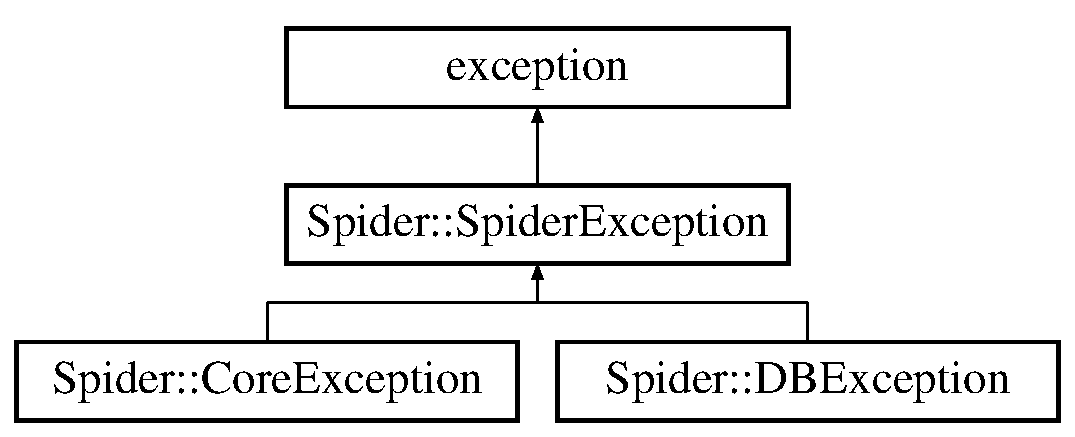
\includegraphics[height=3.000000cm]{class_spider_1_1_spider_exception}
\end{center}
\end{figure}
\subsection*{Public Member Functions}
\begin{DoxyCompactItemize}
\item 
\hyperlink{class_spider_1_1_spider_exception_a00b8eddad95f7872a6d30b5ab11cf3cc}{Spider\+Exception} (const std\+::string \&msg)
\begin{DoxyCompactList}\small\item\em Constructor of the \hyperlink{namespace_spider}{Spider} class Exception by default. \end{DoxyCompactList}\item 
\mbox{\Hypertarget{class_spider_1_1_spider_exception_a173ce8fa7b60115be35381cb103e2f4f}\label{class_spider_1_1_spider_exception_a173ce8fa7b60115be35381cb103e2f4f}} 
virtual \hyperlink{class_spider_1_1_spider_exception_a173ce8fa7b60115be35381cb103e2f4f}{$\sim$\+Spider\+Exception} ()  throw ()
\begin{DoxyCompactList}\small\item\em Destructor of class \hyperlink{class_spider_1_1_spider_exception}{Spider\+Exception}. \end{DoxyCompactList}\item 
virtual const char $\ast$ \hyperlink{class_spider_1_1_spider_exception_aa36edba94a51dc5fb53d54cc98931b2e}{what} () const  throw ()
\begin{DoxyCompactList}\small\item\em Lets you know the identity of the exception. \end{DoxyCompactList}\end{DoxyCompactItemize}


\subsection{Detailed Description}
Exception interface. 

\subsection{Constructor \& Destructor Documentation}
\mbox{\Hypertarget{class_spider_1_1_spider_exception_a00b8eddad95f7872a6d30b5ab11cf3cc}\label{class_spider_1_1_spider_exception_a00b8eddad95f7872a6d30b5ab11cf3cc}} 
\index{Spider\+::\+Spider\+Exception@{Spider\+::\+Spider\+Exception}!Spider\+Exception@{Spider\+Exception}}
\index{Spider\+Exception@{Spider\+Exception}!Spider\+::\+Spider\+Exception@{Spider\+::\+Spider\+Exception}}
\subsubsection{\texorpdfstring{Spider\+Exception()}{SpiderException()}}
{\footnotesize\ttfamily Spider\+::\+Spider\+Exception\+::\+Spider\+Exception (\begin{DoxyParamCaption}\item[{const std\+::string \&}]{msg }\end{DoxyParamCaption})\hspace{0.3cm}{\ttfamily [inline]}}



Constructor of the \hyperlink{namespace_spider}{Spider} class Exception by default. 


\begin{DoxyParams}{Parameters}
{\em msg} & Message related to the exception sent \\
\hline
\end{DoxyParams}


\subsection{Member Function Documentation}
\mbox{\Hypertarget{class_spider_1_1_spider_exception_aa36edba94a51dc5fb53d54cc98931b2e}\label{class_spider_1_1_spider_exception_aa36edba94a51dc5fb53d54cc98931b2e}} 
\index{Spider\+::\+Spider\+Exception@{Spider\+::\+Spider\+Exception}!what@{what}}
\index{what@{what}!Spider\+::\+Spider\+Exception@{Spider\+::\+Spider\+Exception}}
\subsubsection{\texorpdfstring{what()}{what()}}
{\footnotesize\ttfamily virtual const char$\ast$ Spider\+::\+Spider\+Exception\+::what (\begin{DoxyParamCaption}{ }\end{DoxyParamCaption}) const throw  ) \hspace{0.3cm}{\ttfamily [inline]}, {\ttfamily [virtual]}}



Lets you know the identity of the exception. 

\begin{DoxyReturn}{Returns}
Message de l\textquotesingle{}exception 
\end{DoxyReturn}


The documentation for this class was generated from the following file\+:\begin{DoxyCompactItemize}
\item 
Exception/\hyperlink{_spider_exception_8hpp}{Spider\+Exception.\+hpp}\end{DoxyCompactItemize}

\hypertarget{class_spider_1_1_event_1_1_user_activity}{}\section{Spider\+:\+:Event\+:\+:User\+Activity Class Reference}
\label{class_spider_1_1_event_1_1_user_activity}\index{Spider\+::\+Event\+::\+User\+Activity@{Spider\+::\+Event\+::\+User\+Activity}}


\hyperlink{class_spider_1_1_event_1_1_user_activity}{User\+Activity} Handler.  




{\ttfamily \#include $<$User\+Activity.\+hpp$>$}

Inheritance diagram for Spider\+:\+:Event\+:\+:User\+Activity\+:\begin{figure}[H]
\begin{center}
\leavevmode
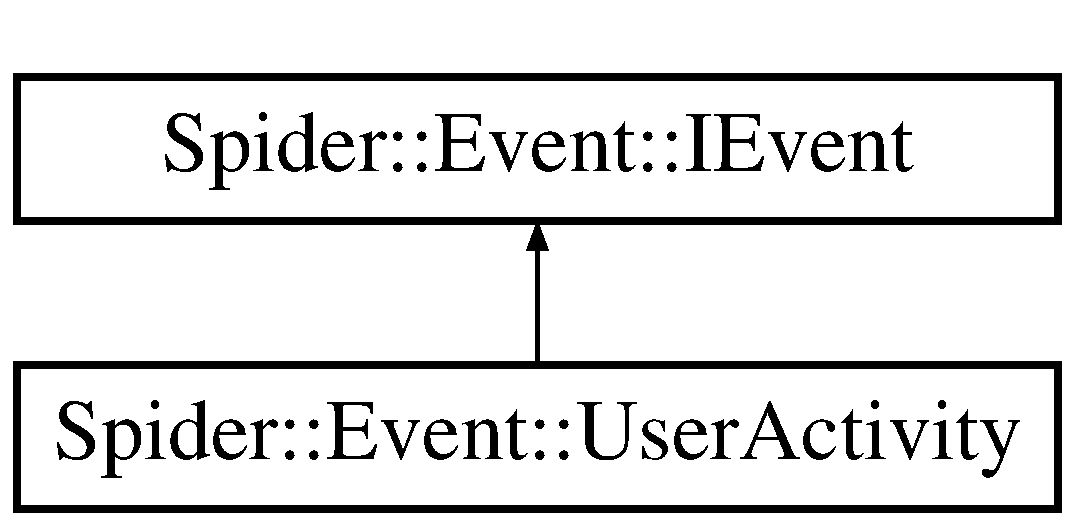
\includegraphics[height=2.000000cm]{class_spider_1_1_event_1_1_user_activity}
\end{center}
\end{figure}
\subsection*{Public Member Functions}
\begin{DoxyCompactItemize}
\item 
\hyperlink{class_spider_1_1_event_1_1_user_activity_a01787e3d65e72b720f322d393e5f7b68}{User\+Activity} (std\+::string activity)
\begin{DoxyCompactList}\small\item\em activity saved \end{DoxyCompactList}\item 
\hyperlink{class_spider_1_1_event_1_1_user_activity_ab7a38e9fbb599851895088657f62915c}{User\+Activity} (const \hyperlink{class_spider_1_1_event_1_1_user_activity}{User\+Activity} \&)=delete
\begin{DoxyCompactList}\small\item\em Default copy constructor. \end{DoxyCompactList}\item 
\hyperlink{class_spider_1_1_event_1_1_user_activity}{User\+Activity} \& \hyperlink{class_spider_1_1_event_1_1_user_activity_a063f3f10b0ecfa7f084a8047e17bea57}{operator=} (const \hyperlink{class_spider_1_1_event_1_1_user_activity}{User\+Activity} \&)=delete
\begin{DoxyCompactList}\small\item\em Operator equal overlaod. \end{DoxyCompactList}\item 
\mbox{\Hypertarget{class_spider_1_1_event_1_1_user_activity_ae793fb71c0316c71f2624f410d4bc697}\label{class_spider_1_1_event_1_1_user_activity_ae793fb71c0316c71f2624f410d4bc697}} 
virtual \hyperlink{class_spider_1_1_event_1_1_user_activity_ae793fb71c0316c71f2624f410d4bc697}{$\sim$\+User\+Activity} ()=default
\begin{DoxyCompactList}\small\item\em Default destroyer. \end{DoxyCompactList}\item 
virtual std\+::string \hyperlink{class_spider_1_1_event_1_1_user_activity_a72d2436a1d9b339cc1cb1950f374562f}{get\+Event\+Info} () const
\begin{DoxyCompactList}\small\item\em Extract \hyperlink{class_spider_1_1_event_1_1_user_activity}{User\+Activity} information. \end{DoxyCompactList}\item 
virtual int \hyperlink{class_spider_1_1_event_1_1_user_activity_aabcbc7060a3f015b71f0b26b475ccf75}{get\+Id} () const
\begin{DoxyCompactList}\small\item\em Get id of the event. \end{DoxyCompactList}\end{DoxyCompactItemize}
\subsection*{Additional Inherited Members}


\subsection{Detailed Description}
\hyperlink{class_spider_1_1_event_1_1_user_activity}{User\+Activity} Handler. 

\subsection{Constructor \& Destructor Documentation}
\mbox{\Hypertarget{class_spider_1_1_event_1_1_user_activity_a01787e3d65e72b720f322d393e5f7b68}\label{class_spider_1_1_event_1_1_user_activity_a01787e3d65e72b720f322d393e5f7b68}} 
\index{Spider\+::\+Event\+::\+User\+Activity@{Spider\+::\+Event\+::\+User\+Activity}!User\+Activity@{User\+Activity}}
\index{User\+Activity@{User\+Activity}!Spider\+::\+Event\+::\+User\+Activity@{Spider\+::\+Event\+::\+User\+Activity}}
\subsubsection{\texorpdfstring{User\+Activity()}{UserActivity()}\hspace{0.1cm}{\footnotesize\ttfamily [1/2]}}
{\footnotesize\ttfamily Spider\+::\+Event\+::\+User\+Activity\+::\+User\+Activity (\begin{DoxyParamCaption}\item[{std\+::string}]{activity }\end{DoxyParamCaption})}



activity saved 

Constructor with the last activity catch \mbox{\Hypertarget{class_spider_1_1_event_1_1_user_activity_ab7a38e9fbb599851895088657f62915c}\label{class_spider_1_1_event_1_1_user_activity_ab7a38e9fbb599851895088657f62915c}} 
\index{Spider\+::\+Event\+::\+User\+Activity@{Spider\+::\+Event\+::\+User\+Activity}!User\+Activity@{User\+Activity}}
\index{User\+Activity@{User\+Activity}!Spider\+::\+Event\+::\+User\+Activity@{Spider\+::\+Event\+::\+User\+Activity}}
\subsubsection{\texorpdfstring{User\+Activity()}{UserActivity()}\hspace{0.1cm}{\footnotesize\ttfamily [2/2]}}
{\footnotesize\ttfamily Spider\+::\+Event\+::\+User\+Activity\+::\+User\+Activity (\begin{DoxyParamCaption}\item[{const \hyperlink{class_spider_1_1_event_1_1_user_activity}{User\+Activity} \&}]{ }\end{DoxyParamCaption})\hspace{0.3cm}{\ttfamily [delete]}}



Default copy constructor. 


\begin{DoxyParams}{Parameters}
{\em last} & activity register \\
\hline
\end{DoxyParams}


\subsection{Member Function Documentation}
\mbox{\Hypertarget{class_spider_1_1_event_1_1_user_activity_a72d2436a1d9b339cc1cb1950f374562f}\label{class_spider_1_1_event_1_1_user_activity_a72d2436a1d9b339cc1cb1950f374562f}} 
\index{Spider\+::\+Event\+::\+User\+Activity@{Spider\+::\+Event\+::\+User\+Activity}!get\+Event\+Info@{get\+Event\+Info}}
\index{get\+Event\+Info@{get\+Event\+Info}!Spider\+::\+Event\+::\+User\+Activity@{Spider\+::\+Event\+::\+User\+Activity}}
\subsubsection{\texorpdfstring{get\+Event\+Info()}{getEventInfo()}}
{\footnotesize\ttfamily virtual std\+::string Spider\+::\+Event\+::\+User\+Activity\+::get\+Event\+Info (\begin{DoxyParamCaption}{ }\end{DoxyParamCaption}) const\hspace{0.3cm}{\ttfamily [virtual]}}



Extract \hyperlink{class_spider_1_1_event_1_1_user_activity}{User\+Activity} information. 

\begin{DoxyReturn}{Returns}
Informations into string format 
\end{DoxyReturn}


Implements \hyperlink{class_spider_1_1_event_1_1_i_event_ac8471df73080237faea55de539d968a0}{Spider\+::\+Event\+::\+I\+Event}.

\mbox{\Hypertarget{class_spider_1_1_event_1_1_user_activity_aabcbc7060a3f015b71f0b26b475ccf75}\label{class_spider_1_1_event_1_1_user_activity_aabcbc7060a3f015b71f0b26b475ccf75}} 
\index{Spider\+::\+Event\+::\+User\+Activity@{Spider\+::\+Event\+::\+User\+Activity}!get\+Id@{get\+Id}}
\index{get\+Id@{get\+Id}!Spider\+::\+Event\+::\+User\+Activity@{Spider\+::\+Event\+::\+User\+Activity}}
\subsubsection{\texorpdfstring{get\+Id()}{getId()}}
{\footnotesize\ttfamily virtual int Spider\+::\+Event\+::\+User\+Activity\+::get\+Id (\begin{DoxyParamCaption}{ }\end{DoxyParamCaption}) const\hspace{0.3cm}{\ttfamily [inline]}, {\ttfamily [virtual]}}



Get id of the event. 

\begin{DoxyReturn}{Returns}
\hyperlink{class_spider_1_1_event_1_1_request}{Request} ID 
\end{DoxyReturn}


Implements \hyperlink{class_spider_1_1_event_1_1_i_event_a902d1376faa8e5948fa5bfe8d7208c88}{Spider\+::\+Event\+::\+I\+Event}.

\mbox{\Hypertarget{class_spider_1_1_event_1_1_user_activity_a063f3f10b0ecfa7f084a8047e17bea57}\label{class_spider_1_1_event_1_1_user_activity_a063f3f10b0ecfa7f084a8047e17bea57}} 
\index{Spider\+::\+Event\+::\+User\+Activity@{Spider\+::\+Event\+::\+User\+Activity}!operator=@{operator=}}
\index{operator=@{operator=}!Spider\+::\+Event\+::\+User\+Activity@{Spider\+::\+Event\+::\+User\+Activity}}
\subsubsection{\texorpdfstring{operator=()}{operator=()}}
{\footnotesize\ttfamily \hyperlink{class_spider_1_1_event_1_1_user_activity}{User\+Activity}\& Spider\+::\+Event\+::\+User\+Activity\+::operator= (\begin{DoxyParamCaption}\item[{const \hyperlink{class_spider_1_1_event_1_1_user_activity}{User\+Activity} \&}]{ }\end{DoxyParamCaption})\hspace{0.3cm}{\ttfamily [delete]}}



Operator equal overlaod. 

\begin{DoxyReturn}{Returns}
\hyperlink{class_spider_1_1_event_1_1_user_activity}{User\+Activity} 
\end{DoxyReturn}


The documentation for this class was generated from the following file\+:\begin{DoxyCompactItemize}
\item 
Event/\hyperlink{_user_activity_8hpp}{User\+Activity.\+hpp}\end{DoxyCompactItemize}

\chapter{File Documentation}
\hypertarget{_key_reader_8hpp}{}\section{Core/\+Key\+Reader.hpp File Reference}
\label{_key_reader_8hpp}\index{Core/\+Key\+Reader.\+hpp@{Core/\+Key\+Reader.\+hpp}}
{\ttfamily \#include $<$string$>$}\newline
{\ttfamily \#include $<$vector$>$}\newline
{\ttfamily \#include \char`\"{}Event/\+I\+Event.\+hpp\char`\"{}}\newline
{\ttfamily \#include $<$windows.\+h$>$}\newline
\subsection*{Classes}
\begin{DoxyCompactItemize}
\item 
class \hyperlink{class_spider_1_1_core_1_1_key_reader}{Spider\+::\+Core\+::\+Key\+Reader}
\begin{DoxyCompactList}\small\item\em Read event. \end{DoxyCompactList}\end{DoxyCompactItemize}
\subsection*{Namespaces}
\begin{DoxyCompactItemize}
\item 
 \hyperlink{namespace_spider}{Spider}
\end{DoxyCompactItemize}
\subsection*{Functions}
\begin{DoxyCompactItemize}
\item 
\mbox{\Hypertarget{_key_reader_8hpp_a4acc05463acf0f89648a3e868ad15706}\label{_key_reader_8hpp_a4acc05463acf0f89648a3e868ad15706}} 
const std\+::vector$<$ int $>$ \hyperlink{_key_reader_8hpp_a4acc05463acf0f89648a3e868ad15706}{Spider\+::\+Core\+::m\+Ignored\+Char} (\{ V\+K\+\_\+\+R\+C\+O\+N\+T\+R\+OL, V\+K\+\_\+\+L\+C\+O\+N\+T\+R\+OL, V\+K\+\_\+\+L\+M\+E\+NU, V\+K\+\_\+\+R\+S\+H\+I\+FT, V\+K\+\_\+\+L\+S\+H\+I\+FT \})
\begin{DoxyCompactList}\small\item\em Key to ignored. \end{DoxyCompactList}\end{DoxyCompactItemize}
\subsection*{Variables}
\begin{DoxyCompactItemize}
\item 
\mbox{\Hypertarget{_key_reader_8hpp_aa5f171789fe5d11ea8adfafe8f241006}\label{_key_reader_8hpp_aa5f171789fe5d11ea8adfafe8f241006}} 
const int \hyperlink{_key_reader_8hpp_aa5f171789fe5d11ea8adfafe8f241006}{Spider\+::\+Core\+::\+Is\+The\+Touch} = -\/32767
\begin{DoxyCompactList}\small\item\em Value use by the function Get\+Async\+Key() to verify if a key is pressed. \end{DoxyCompactList}\end{DoxyCompactItemize}


\subsection{Detailed Description}
\begin{DoxyAuthor}{Author}
mliani 
\end{DoxyAuthor}
\begin{DoxyDate}{Date}
30/09/2017 
\end{DoxyDate}

\hypertarget{_spider_8hpp}{}\section{Core/\+Spider.hpp File Reference}
\label{_spider_8hpp}\index{Core/\+Spider.\+hpp@{Core/\+Spider.\+hpp}}
{\ttfamily \#include \char`\"{}Event/\+Event\+Queue.\+hpp\char`\"{}}\newline
\subsection*{Classes}
\begin{DoxyCompactItemize}
\item 
class \hyperlink{class_spider_1_1_core_1_1_spider}{Spider\+::\+Core\+::\+Spider}
\begin{DoxyCompactList}\small\item\em Project main class. \end{DoxyCompactList}\end{DoxyCompactItemize}
\subsection*{Namespaces}
\begin{DoxyCompactItemize}
\item 
 \hyperlink{namespace_spider}{Spider}
\end{DoxyCompactItemize}


\subsection{Detailed Description}
\begin{DoxyAuthor}{Author}
jbruel 
\end{DoxyAuthor}
\begin{DoxyDate}{Date}
30/09/2017 
\end{DoxyDate}

\hypertarget{_d_b_handler_8hpp}{}\section{D\+B/\+D\+B\+Handler.hpp File Reference}
\label{_d_b_handler_8hpp}\index{D\+B/\+D\+B\+Handler.\+hpp@{D\+B/\+D\+B\+Handler.\+hpp}}
{\ttfamily \#include $<$sqlite3.\+h$>$}\newline
{\ttfamily \#include $<$memory$>$}\newline
{\ttfamily \#include $<$string$>$}\newline
{\ttfamily \#include \char`\"{}Event/\+Request.\+hpp\char`\"{}}\newline
\subsection*{Classes}
\begin{DoxyCompactItemize}
\item 
class \hyperlink{class_spider_1_1_d_b_1_1_d_b_handler}{Spider\+::\+D\+B\+::\+D\+B\+Handler}
\end{DoxyCompactItemize}
\subsection*{Namespaces}
\begin{DoxyCompactItemize}
\item 
 \hyperlink{namespace_spider}{Spider}
\end{DoxyCompactItemize}


\subsection{Detailed Description}
\begin{DoxyAuthor}{Author}
aiacona 
\end{DoxyAuthor}
\begin{DoxyDate}{Date}
03/10/2017 
\end{DoxyDate}

\hypertarget{_click_association_8hpp}{}\section{Event/\+Click\+Association.hpp File Reference}
\label{_click_association_8hpp}\index{Event/\+Click\+Association.\+hpp@{Event/\+Click\+Association.\+hpp}}
{\ttfamily \#include $<$unordered\+\_\+map$>$}\newline
{\ttfamily \#include \char`\"{}Event/\+I\+Event.\+hpp\char`\"{}}\newline
\subsection*{Namespaces}
\begin{DoxyCompactItemize}
\item 
 \hyperlink{namespace_spider}{Spider}
\item 
 \hyperlink{namespace_spider_1_1_event}{Spider\+::\+Event}
\end{DoxyCompactItemize}
\subsection*{Variables}
\begin{DoxyCompactItemize}
\item 
std\+::unordered\+\_\+map$<$ int, Event\+::\+Click\+Type $>$ {\bfseries Spider\+::\+Event\+::associative\+Click}
\end{DoxyCompactItemize}


\subsection{Detailed Description}
\begin{DoxyAuthor}{Author}
mliani 
\end{DoxyAuthor}
\begin{DoxyDate}{Date}
30/09/2017 
\end{DoxyDate}

\hypertarget{_event_8hpp}{}\section{Event/\+Event.hpp File Reference}
\label{_event_8hpp}\index{Event/\+Event.\+hpp@{Event/\+Event.\+hpp}}
{\ttfamily \#include \char`\"{}Event/\+Click.\+hpp\char`\"{}}\newline
{\ttfamily \#include \char`\"{}Event/\+User\+Activity.\+hpp\char`\"{}}\newline
{\ttfamily \#include \char`\"{}Event/\+Keyboard.\+hpp\char`\"{}}\newline
{\ttfamily \#include \char`\"{}Event/\+Event\+Queue.\+hpp\char`\"{}}\newline
{\ttfamily \#include \char`\"{}Event/\+Event\+Handler.\+hpp\char`\"{}}\newline
{\ttfamily \#include \char`\"{}Event/\+Click\+Association.\+hpp\char`\"{}}\newline


\subsection{Detailed Description}
\begin{DoxyAuthor}{Author}
mliani 
\end{DoxyAuthor}
\begin{DoxyDate}{Date}
30/09/2017 
\end{DoxyDate}

\hypertarget{_event_handler_8hpp}{}\section{Event/\+Event\+Handler.hpp File Reference}
\label{_event_handler_8hpp}\index{Event/\+Event\+Handler.\+hpp@{Event/\+Event\+Handler.\+hpp}}
{\ttfamily \#include $<$memory$>$}\newline
{\ttfamily \#include \char`\"{}Event/\+I\+Event.\+hpp\char`\"{}}\newline
{\ttfamily \#include \char`\"{}ssl/\+R\+S\+A\+Keys.\+hpp\char`\"{}}\newline
{\ttfamily \#include \char`\"{}Socket/\+Tcp\+Client\+Socket.\+hpp\char`\"{}}\newline
{\ttfamily \#include \char`\"{}D\+B/\+D\+B\+Handler.\+hpp\char`\"{}}\newline
{\ttfamily \#include \char`\"{}Socket/\+Packet\+Manager.\+hpp\char`\"{}}\newline
{\ttfamily \#include \char`\"{}Exception/\+D\+B\+Exception.\+hpp\char`\"{}}\newline
{\ttfamily \#include $<$boost/asio.\+hpp$>$}\newline
{\ttfamily \#include $<$windows.\+h$>$}\newline
\subsection*{Classes}
\begin{DoxyCompactItemize}
\item 
class \hyperlink{class_spider_1_1_event_1_1_event_handler}{Spider\+::\+Event\+::\+Event\+Handler}
\begin{DoxyCompactList}\small\item\em Handle events. \end{DoxyCompactList}\end{DoxyCompactItemize}
\subsection*{Namespaces}
\begin{DoxyCompactItemize}
\item 
 \hyperlink{namespace_spider}{Spider}
\item 
 \hyperlink{namespace_spider_1_1_event}{Spider\+::\+Event}
\end{DoxyCompactItemize}


\subsection{Detailed Description}
\begin{DoxyAuthor}{Author}
jbruel 
\end{DoxyAuthor}
\begin{DoxyDate}{Date}
01/10/2017
\end{DoxyDate}
\begin{DoxyAuthor}{Author}
jbruel 
\end{DoxyAuthor}
\begin{DoxyDate}{Date}
03/10/2017 
\end{DoxyDate}

\hypertarget{_event_queue_8hpp}{}\section{Event/\+Event\+Queue.hpp File Reference}
\label{_event_queue_8hpp}\index{Event/\+Event\+Queue.\+hpp@{Event/\+Event\+Queue.\+hpp}}
{\ttfamily \#include $<$mutex$>$}\newline
{\ttfamily \#include $<$vector$>$}\newline
{\ttfamily \#include \char`\"{}Event/\+I\+Event.\+hpp\char`\"{}}\newline
\subsection*{Classes}
\begin{DoxyCompactItemize}
\item 
class \hyperlink{class_spider_1_1_event_1_1_event_queue}{Spider\+::\+Event\+::\+Event\+Queue}
\begin{DoxyCompactList}\small\item\em Queue system for \hyperlink{namespace_spider}{Spider} events. \end{DoxyCompactList}\end{DoxyCompactItemize}
\subsection*{Namespaces}
\begin{DoxyCompactItemize}
\item 
 \hyperlink{namespace_spider}{Spider}
\item 
 \hyperlink{namespace_spider_1_1_event}{Spider\+::\+Event}
\end{DoxyCompactItemize}


\subsection{Detailed Description}
\begin{DoxyAuthor}{Author}
jbruel 
\end{DoxyAuthor}
\begin{DoxyDate}{Date}
30/09/2017 
\end{DoxyDate}

\hypertarget{_i_event_8hpp}{}\section{Event/\+I\+Event.hpp File Reference}
\label{_i_event_8hpp}\index{Event/\+I\+Event.\+hpp@{Event/\+I\+Event.\+hpp}}
{\ttfamily \#include $<$string$>$}\newline
\subsection*{Classes}
\begin{DoxyCompactItemize}
\item 
struct \hyperlink{struct_spider_1_1_event_1_1_click_coord}{Spider\+::\+Event\+::\+Click\+Coord}
\begin{DoxyCompactList}\small\item\em Define the click coordonate. \end{DoxyCompactList}\item 
class \hyperlink{class_spider_1_1_event_1_1_i_event}{Spider\+::\+Event\+::\+I\+Event}
\begin{DoxyCompactList}\small\item\em \hyperlink{namespace_spider_1_1_event}{Event} interface. \end{DoxyCompactList}\end{DoxyCompactItemize}
\subsection*{Namespaces}
\begin{DoxyCompactItemize}
\item 
 \hyperlink{namespace_spider}{Spider}
\item 
 \hyperlink{namespace_spider_1_1_event}{Spider\+::\+Event}
\end{DoxyCompactItemize}
\subsection*{Enumerations}
\begin{DoxyCompactItemize}
\item 
\mbox{\Hypertarget{namespace_spider_1_1_event_ae178d39ebb8937d04ffe6ead8f306fd0}\label{namespace_spider_1_1_event_ae178d39ebb8937d04ffe6ead8f306fd0}} 
enum \hyperlink{namespace_spider_1_1_event_ae178d39ebb8937d04ffe6ead8f306fd0}{Spider\+::\+Event\+::\+Click\+Type} \{ {\bfseries L\+E\+F\+T\+\_\+\+C\+L\+I\+CK}, 
{\bfseries M\+I\+D\+D\+L\+E\+\_\+\+C\+L\+I\+CK}, 
{\bfseries R\+I\+G\+H\+T\+\_\+\+C\+L\+I\+CK}, 
{\bfseries N\+O\+NE}
 \}\begin{DoxyCompactList}\small\item\em Define the type of the click from the user. \end{DoxyCompactList}
\end{DoxyCompactItemize}


\subsection{Detailed Description}
\begin{DoxyAuthor}{Author}
mliani 
\end{DoxyAuthor}
\begin{DoxyDate}{Date}
30/09/2017 
\end{DoxyDate}

\hypertarget{_user_activity_8hpp}{}\section{Event/\+User\+Activity.hpp File Reference}
\label{_user_activity_8hpp}\index{Event/\+User\+Activity.\+hpp@{Event/\+User\+Activity.\+hpp}}
{\ttfamily \#include \char`\"{}Event/\+I\+Event.\+hpp\char`\"{}}\newline
\subsection*{Classes}
\begin{DoxyCompactItemize}
\item 
class \hyperlink{class_spider_1_1_event_1_1_user_activity}{Spider\+::\+Event\+::\+User\+Activity}
\begin{DoxyCompactList}\small\item\em \hyperlink{class_spider_1_1_event_1_1_user_activity}{User\+Activity} Handler. \end{DoxyCompactList}\end{DoxyCompactItemize}
\subsection*{Namespaces}
\begin{DoxyCompactItemize}
\item 
 \hyperlink{namespace_spider}{Spider}
\item 
 \hyperlink{namespace_spider_1_1_event}{Spider\+::\+Event}
\end{DoxyCompactItemize}


\subsection{Detailed Description}
\begin{DoxyAuthor}{Author}
mliani 
\end{DoxyAuthor}
\begin{DoxyDate}{Date}
30/09/2017 
\end{DoxyDate}

\hypertarget{_core_exception_8hpp}{}\section{Exception/\+Core\+Exception.hpp File Reference}
\label{_core_exception_8hpp}\index{Exception/\+Core\+Exception.\+hpp@{Exception/\+Core\+Exception.\+hpp}}
{\ttfamily \#include \char`\"{}Spider\+Exception.\+hpp\char`\"{}}\newline
\subsection*{Classes}
\begin{DoxyCompactItemize}
\item 
class \hyperlink{class_spider_1_1_core_exception}{Spider\+::\+Core\+Exception}
\begin{DoxyCompactList}\small\item\em Core exception class. \end{DoxyCompactList}\end{DoxyCompactItemize}
\subsection*{Namespaces}
\begin{DoxyCompactItemize}
\item 
 \hyperlink{namespace_spider}{Spider}
\end{DoxyCompactItemize}


\subsection{Detailed Description}
\begin{DoxyAuthor}{Author}
jbruel 
\end{DoxyAuthor}
\begin{DoxyDate}{Date}
26/09/2017 
\end{DoxyDate}

\hypertarget{_d_b_exception_8hpp}{}\section{Exception/\+D\+B\+Exception.hpp File Reference}
\label{_d_b_exception_8hpp}\index{Exception/\+D\+B\+Exception.\+hpp@{Exception/\+D\+B\+Exception.\+hpp}}
{\ttfamily \#include \char`\"{}Spider\+Exception.\+hpp\char`\"{}}\newline
\subsection*{Classes}
\begin{DoxyCompactItemize}
\item 
class \hyperlink{class_spider_1_1_d_b_exception}{Spider\+::\+D\+B\+Exception}
\end{DoxyCompactItemize}
\subsection*{Namespaces}
\begin{DoxyCompactItemize}
\item 
 \hyperlink{namespace_spider}{Spider}
\end{DoxyCompactItemize}


\subsection{Detailed Description}
\begin{DoxyAuthor}{Author}
jbruel 
\end{DoxyAuthor}
\begin{DoxyDate}{Date}
03/10/2017 
\end{DoxyDate}

\hypertarget{_spider_exception_8hpp}{}\section{Exception/\+Spider\+Exception.hpp File Reference}
\label{_spider_exception_8hpp}\index{Exception/\+Spider\+Exception.\+hpp@{Exception/\+Spider\+Exception.\+hpp}}
{\ttfamily \#include $<$string$>$}\newline
{\ttfamily \#include $<$exception$>$}\newline
\subsection*{Classes}
\begin{DoxyCompactItemize}
\item 
class \hyperlink{class_spider_1_1_spider_exception}{Spider\+::\+Spider\+Exception}
\begin{DoxyCompactList}\small\item\em Exception interface. \end{DoxyCompactList}\end{DoxyCompactItemize}
\subsection*{Namespaces}
\begin{DoxyCompactItemize}
\item 
 \hyperlink{namespace_spider}{Spider}
\end{DoxyCompactItemize}


\subsection{Detailed Description}
\begin{DoxyAuthor}{Author}
jbruel 
\end{DoxyAuthor}
\begin{DoxyDate}{Date}
26/09/2017 
\end{DoxyDate}

\hypertarget{_a_e_s_8hpp}{}\section{ssl/\+A\+ES.hpp File Reference}
\label{_a_e_s_8hpp}\index{ssl/\+A\+E\+S.\+hpp@{ssl/\+A\+E\+S.\+hpp}}
{\ttfamily \#include $<$string$>$}\newline
{\ttfamily \#include $<$cstring$>$}\newline
{\ttfamily \#include $<$openssl/rand.\+h$>$}\newline
{\ttfamily \#include $<$openssl/aes.\+h$>$}\newline
\subsection*{Classes}
\begin{DoxyCompactItemize}
\item 
class \hyperlink{class_spider_1_1ssl_1_1_a_e_s}{Spider\+::ssl\+::\+A\+ES}
\begin{DoxyCompactList}\small\item\em Encapsulation of the open\+S\+SL \hyperlink{class_spider_1_1ssl_1_1_a_e_s}{A\+ES} system. \end{DoxyCompactList}\end{DoxyCompactItemize}
\subsection*{Namespaces}
\begin{DoxyCompactItemize}
\item 
 \hyperlink{namespace_spider}{Spider}
\end{DoxyCompactItemize}


\subsection{Detailed Description}
\begin{DoxyAuthor}{Author}
jbruel 
\end{DoxyAuthor}
\begin{DoxyDate}{Date}
30/09/2017 
\end{DoxyDate}

\hypertarget{_r_s_a_keys_8hpp}{}\section{ssl/\+R\+S\+A\+Keys.hpp File Reference}
\label{_r_s_a_keys_8hpp}\index{ssl/\+R\+S\+A\+Keys.\+hpp@{ssl/\+R\+S\+A\+Keys.\+hpp}}
{\ttfamily \#include $<$string$>$}\newline
{\ttfamily \#include $<$openssl\textbackslash{}rsa.\+h$>$}\newline
\subsection*{Classes}
\begin{DoxyCompactItemize}
\item 
class \hyperlink{class_spider_1_1ssl_1_1_r_s_a_keys}{Spider\+::ssl\+::\+R\+S\+A\+Keys}
\begin{DoxyCompactList}\small\item\em Encapsulation of the open\+S\+SL one-\/way encryption system. \end{DoxyCompactList}\end{DoxyCompactItemize}
\subsection*{Namespaces}
\begin{DoxyCompactItemize}
\item 
 \hyperlink{namespace_spider}{Spider}
\end{DoxyCompactItemize}


\subsection{Detailed Description}
\begin{DoxyAuthor}{Author}
jbruel 
\end{DoxyAuthor}
\begin{DoxyDate}{Date}
26/09/2017 
\end{DoxyDate}

\hypertarget{_sha_8hpp}{}\section{ssl/\+Sha.hpp File Reference}
\label{_sha_8hpp}\index{ssl/\+Sha.\+hpp@{ssl/\+Sha.\+hpp}}
{\ttfamily \#include $<$openssl/sha.\+h$>$}\newline
{\ttfamily \#include $<$cstdlib$>$}\newline
{\ttfamily \#include $<$cstring$>$}\newline
\subsection*{Classes}
\begin{DoxyCompactItemize}
\item 
class \hyperlink{class_spider_1_1ssl_1_1_sha}{Spider\+::ssl\+::\+Sha}
\begin{DoxyCompactList}\small\item\em Encapsulation of the open\+S\+SL one-\/way encryption system. \end{DoxyCompactList}\end{DoxyCompactItemize}
\subsection*{Namespaces}
\begin{DoxyCompactItemize}
\item 
 \hyperlink{namespace_spider}{Spider}
\end{DoxyCompactItemize}


\subsection{Detailed Description}
\begin{DoxyAuthor}{Author}
jbruel 
\end{DoxyAuthor}
\begin{DoxyDate}{Date}
23/08/2017 
\end{DoxyDate}

\hypertarget{ssl_8hpp}{}\section{ssl/ssl.hpp File Reference}
\label{ssl_8hpp}\index{ssl/ssl.\+hpp@{ssl/ssl.\+hpp}}
{\ttfamily \#include \char`\"{}R\+S\+A\+Keys.\+hpp\char`\"{}}\newline
{\ttfamily \#include \char`\"{}Sha.\+hpp\char`\"{}}\newline
{\ttfamily \#include \char`\"{}A\+E\+S.\+hpp\char`\"{}}\newline


\subsection{Detailed Description}
\begin{DoxyAuthor}{Author}
jbruel 
\end{DoxyAuthor}
\begin{DoxyDate}{Date}
27/09/2017 
\end{DoxyDate}

%--- End generated contents ---

% Index
\backmatter
\newpage
\phantomsection
\clearemptydoublepage
\addcontentsline{toc}{chapter}{Index}
\printindex

\end{document}
